\chapter{Application Security}
\label{ch:application-security}

\section{Decentralised Finance}
One of the major applications of blockchain systems, and Ethereum in particular is decentralized finance, often referred to as DeFi.
DeFi is the development of financial systems on top of blockchains using smart contracts.
DeFi systems have several major characteristics:
\begin{description}
  \setlength{\baselineskip}{15pt}
\item[Non-custodial] Users of DeFi systems should have control over their funds at all time
\item[Permisionless] DeFi systems should be available to everyone
\item[Openly auditable] Anyone has the ability to verify the state of a DeFi system at any point in time
\item[Composable] DeFi systems can be freely composed to interact with one another.
\end{description}

There are several primitive, in the form of smart contracts, that are often used when building DeFi systems.

\subsection{Oracles}
One of the major challenges smart contracts face concerns access to off-chain information, i.e. data that does not natively exist on-chain.
Oracles are data feeds into smart contracts and provide a mechanism for accessing off-chain information through some third party.
In DeFi, oracles are commonly used for price feed data to determine the real-time price of assets.
For instance, via the Compound Open Price Feed~\cite{web:compoundfinance_prices}, vetted third-party reporters sign off on price data using a known public key, where the resulting feed can be relied upon by smart contracts.

\subsection{Stablecoins}
An alternative to volatile cryptoassets is given by stablecoins, which are priced against a peg and can be either custodial or non-custodial.
For custodial stablecoins (e.g. \coin{USDC}~\cite{web:usdc}), tokens represent a claim of some off-chain reserve asset, such as fiat currency, which has been entrusted to a custodian.
Non-custodial stablecoins (e.g. \coin{DAI}~\cite{whitepaper:maker}) seek to establish price stability via economic mechanisms specified by smart contracts.
For a thorough discussion on stablecoin design, we direct the reader to \cite{Klages-Mundt2020}.


\section{Smart Contracts Security}
While most of the work related to technical security has focused on detecting \emph{vulnerable} contracts, in this part of the chapter, we focus on finding out how many of these vulnerable contracts have actually been \emph{exploited}.
We survey the~\VulnerableContracts vulnerable contracts reported by~\PapersAnalyzed recent academic projects and find that, despite the amounts at stake, only~\PercentExploitedContracts of them have been exploited since deployment.
This corresponds to at most~\ExploitedEther ETH (\textasciitilde\ExploitedEtherUSD USD\footnotemark), or only~\PercentExploitedEther of the \EtherClaimedVulnerable ETH (\EtherClaimedVulnerableUSD USD) at stake.
We explain these results by demonstrating that the funds are very concentrated in a small number of contracts which are \emph{not exploitable} in practice.

\subsection{Introduction}
\label{sec:5a:introduction}

When it comes to vulnerability research, especially as it pertains to software security, it is frequently difficult to estimate what fraction of discovered vulnerabilities are exploited in practice. However, public blockchains, with their immutability, ease of access, and what amounts to a replayable execution log for smart contracts present an excellent opportunity for such an investigation. 
In this work, we aim to contrast the vulnerabilities reported in smart contracts on the Ethereum~\cite{buterin2014} blockchain with the actual exploitation of these contracts.

We collect the data shared with us by the authors of~\PapersAnalyzed recent papers~\cite{luu2016a,DBLP:conf/ndss/KalraGDS18,Tsankov2018,Grech2018,Nikolic2018a,Krupp2018} that focus on finding smart contract vulnerabilities. These academic datasets are significantly bigger in scale than reports we can find in the wild and because of the sheer number of affected contracts~---~\VulnerableContracts~---~represent an excellent study subject. 

To make our approach more general, we express~\VulnTypes different frequently reported vulnerability classes as Datalog queries computed over relations that represent the state of the Ethereum blockchain. The Datalog-based exploit discovery approach gives more scalability to our process; also, while others have used Datalog for static analysis formulation, we are not aware of it being used to capture the dynamic state of the blockchain over time.

We discover that the amount of smart contract exploitation which occurs in the wild is notably lower than what might be believed, given what is suggested by the sometimes sensational nature of some of the famous cryptocurrency exploits such as TheDAO~\cite{securities2017} or the Parity wallet~\cite{Breidenbach} bugs.

\point{Contributions} Our contributions are:\itemsep=0pt
\begin{itemize}\itemsep=-2pt
% \item
\item \textbf{Datalog formulation.}
    We propose a Datalog-based formulation for performing analysis over Ethereum Virtual Machine (EVM) execution traces. We use this highly scalable approach to analyze a total of more than~\empirical{20 million} transactions from the Ethereum blockchain to search for exploits. We highlight that our analyses run \emph{automatically} using data extracted from the transactions and the Datalog rules that we define in this chapter.

\item \textbf{Experimental evaluation of exploitation.}
    We analyze the vulnerabilities reported in \PapersAnalyzed recently published studies and conclude that, although the number of \emph{vulnerable} contracts and the amount of money at risk is very high, the amount of money actually \emph{exploited} is several orders of magnitude lower.

    We discover that out of~\empirical{\VulnerableContracts} vulnerable contracts worth a total of~\empirical{\EtherStake} ETH,~\empirical{\NumExploitedContracts} contracts may have been exploited for an amount of~\empirical{\ExploitedEther} ETH, which represents only~\empirical{\PercentExploitedEther} of the total amount at stake.

\item \textbf{Proposed explanations.}
    We hypothesise that the main reason for these vast differences is that the amount of \emph{exploitable} Ether is very low compared to the amount of Ether flagged \emph{vulnerable}.
    Indeed, further analysis of the vulnerable contracts and the Ether they contain suggests that a large majority of Ether is held by only a small number of contracts and that the vulnerabilities reported on these contracts are either false positives or not exploitable in practice. We also confirm that the set of all contracts on the Ethereum blockchain has a similar distribution of wealth to our dataset.
\end{itemize}
To make many of the discussions in this chapter more concrete, we present a thorough investigation of the high-value contracts in \autoref{sec:5a:discussion}. 


\subsection{Background}
\label{sec:5a:background} 
In this section, we first introduce different types of smart contract vulnerabilities.
We then present some of the analysis tools available to prevent such vulnerabilities.
Finally, we provide some definitions that will be used in the rest of the chapter.

\subsubsection{Smart Contracts Vulnerabilities}
\label{ssec:vulnerability-types}
In this subsection, we briefly review some of the most common vulnerability types that have been researched and reported for EVM-based smart contracts.
We provide a two-letter abbreviation for each vulnerability which we shall use throughout the remainder of this section.

\point{\reentrancy~(\vre)}
When a contract ``calls'' another account, it can choose the amount of gas it allows the called party to use. If the target account is a contract, it will be executed and can use the provided gas budget. If such a contract is malicious and the gas budget is high enough, it can try to call back from the caller --- a re-entrant call. If the caller's implementation is not re-entrant, for example, because it did not update his internal state containing balances information, the attacker can use this vulnerability to drain funds out of the vulnerable contract~\cite{Luu2016a,DBLP:conf/ndss/KalraGDS18,Tsankov2018}.
This vulnerability was used in TheDAO exploit~\cite{Securities2017}, essentially causing the Ethereum community to decide to roll back to a previous state using a hard-fork~\cite{mehar2019understanding}. We provide more details about TheDAO exploit in Section~\ref{sec:5a:related}

\point{\unhandledexceptions~(\vue)}
Some low-level operations in Solidity such as \lstinline{send}, which is used to send Ether, do not throw an exception on failure, but rather report the status by returning a boolean.
If this return value is unchecked, the caller continues its execution even if the payment failed, which can easily lead to inconsistencies~\cite{Brent2018,Luu2016a,Tikhomirov2017,DBLP:conf/ndss/KalraGDS18}.

\point{\lockedether~(\vle)}
Ethereum smart contracts can, as any account on Ethereum, receive Ether. However, there as several reasons causing the received funds to get locked permanently into the contract.

One reason is that the contract may depend on another contract which has been
destructed using the \op{SELFDESTRUCT} instruction of the EVM --- i.e. its code has been removed and its funds transferred. If this was the only way for such a contract to send Ether, it will result in the funds being permanently locked. This is what happened in the Parity Wallet bug in November 2017, locking millions of USD worth of Ether~\cite{Breidenbach}. We provide more details about the Parity Wallet bug in Section~\ref{sec:5a:related}

There are also cases where the contract will \emph{always} run out of gas when trying
to send Ether which could result in locking the contract funds. More details about such issues can be found in~\cite{Grech2018}.

\point{\transactionorder~(\vto)}
In Ethereum, multiple transactions are included in a single block, which means that the state of a contract can be updated multiple times in the same block. If the order of two transactions calling the same smart contract changes the outcome, an attacker could exploit this property. 
For example, given a contract which expects participants to submit the solution to a puzzle in exchange for a reward, a malicious contract owner could reduce the amount of the reward when the transaction is submitted.

\point{\integeroverflow~(\vio)}
Integer overflow and underflow are common types of bugs in many programming languages but in the context of Ethereum, they can have very severe consequences. For example, if a loop counter were to overflow, creating an infinite loop, the funds of a contract could become completely frozen. This can be exploited by an attacker if he has a way of incrementing the number of iterations of the loop, for example, by registering enough users to trigger an overflow.

\point{\unrestrictedaction~(\vua)}
Contracts often perform authorization, by checking the sender of the message, to restrict the type of action that a user can take.
Typically, only the owner of a contract should be allowed to destroy the contract or set a new owner.
This owner is usually set in the contract constructor but some contracts were found vulnerable because the owner was not initialized correctly, allowing, for example, an attacker to take ownership of the contract.
A reason for such a bug could be a misnamed function in older versions of Solidity~\cite{Brent2018,Krupp2018}.
This issue was the root cause of the the Parity wallet bug~\cite{Tsankov2018,Nikolic2018a} which froze more than 500k Ether.

Such an issue can happen not only if the developer forgets to perform critical checks but also if an attacker can execute arbitrary code, for example by being able to control the address of a delegated call~\cite{Krupp2018}.


\begin{table}[tb]
  \centering
  \caption{A summary of smart contract analysis tools presented in prior work.}
  \label{fig:prior-results}
  \setlength{\tabcolsep}{2pt}
  \small
  \begin{tabular}{lp{10mm}p{10mm}p{10mm}p{10mm}p{10mm}p{10mm}cc}
    \toprule
    \multirow{2}{*}{\bf Name} & \multicolumn{6}{c}{\bf Vulnerabilities} & \bf Report & \multirow{2}{*}{\bf  Citation}                                                                                       \\
                              & \vre                                    & \vue       & \vle                           & \vto       & \vio       & \vua       & \bf month &                                  \\
    \midrule
    Oyente                    & \checkmark                              & \checkmark &                                & \checkmark & \checkmark &            & 2016-10   & \cite{Luu2016a}                  \\ \midrule
    ZEUS                      & \checkmark                              & \checkmark & \checkmark                     & \checkmark & \checkmark &            & 2018-02   & \cite{DBLP:conf/ndss/KalraGDS18} \\ \midrule
    Maian                     &                                         &            & \checkmark                     &            &            & \checkmark & 2018-03   & \cite{Nikolic2018a}              \\ \midrule
    SmartCheck                & \checkmark                              & \checkmark & \checkmark                     &            & \checkmark &            & 2018-05   & \cite{Tikhomirov2017}            \\ \midrule
    Securify                  & \checkmark                              & \checkmark & \checkmark                     & \checkmark &            & \checkmark & 2018-06   & \cite{Tsankov2018}               \\ \midrule
    ContractFuzzer            & \checkmark                              & \checkmark &                                &            &            &            & 2018-09   & \cite{Jiang2018}                 \\ \midrule
    teEther                   &                                         &            &                                &            &            & \checkmark & 2018-08   & \cite{Krupp2018}                 \\ \midrule
    Vandal                    & \checkmark                              & \checkmark &                                &            &            &            & 2018-09   & \cite{Brent2018}                 \\ \midrule
    MadMax                    &                                         &            & \checkmark                     &            & \checkmark &            & 2018-10   & \cite{Grech2018}                 \\
    \bottomrule
  \end{tabular}
\end{table}

\subsubsection{Analysis Tools}
\label{ssec:analysis-tools}
Smart contracts are generally designed to manipulate and \emph{hold} funds denominated in Ether. This makes them very tempting attack targets, as a successful attack may allow the attacker to directly steal funds from the contract.
Given the many common vulnerabilities in smart contracts, some of which we described in the previous section, a large number of tools have been developed to find them automatically~\cite{Luu2016a,Tsankov2018,mythril}.
Most of these tools analyze either the contract source code or its compiled EVM bytecode and look for known security issues, such as re-entrancy or transaction order dependency vulnerabilities. We present a summary of these different works in Figure~\ref{fig:prior-results}. The second and third columns respectively present the reported number of contracts analyzed and contracts flagged as vulnerable in each paper. The ``vulnerabilities'' columns show the type of vulnerabilities that each tool can check for. We present these vulnerabilities in Subsection~\ref{ssec:vulnerability-types} and give a more detailed description of these tools in Section~\ref{sec:5a:related}.

\point{Testing}
Like any piece of software, smart contracts benefit from automated testing and some efforts have therefore been made to make the testing experience more straightforward. Truffle~\cite{truffle} is a popular framework for developing smart contracts, which allows writing both unit and integration tests for smart contracts in JavaScript. One difficulty of testing on the Ethereum platform is that the EVM does not have a single main entry point and bytecode is executed when fulfilling a transaction. Some tools, such as standalone EVM implementations~\cite{ganache} have been developed to ease this process.

\point{Auditing}
As smart contracts can have a high monetary value, \emph{auditing} contracts for vulnerabilities is a common industrial practice.
Audits should preferably be performed while contracts are still in the testing phase but given the relatively high cost of auditing (usually around 30,000 to 40,000 USD~\cite{solidified}) some companies choose to perform audits later in their development cycle. In addition to checking for common vulnerabilities and implementation issues such as gas-consuming operations, audits also usually check for divergences from specifications and other high-level logic errors, which are impossible for current automatic tools to detect.

\point{Bounty programs}
Another common practice for developers to improve the security of their smart contracts is to run bounty programs. While auditing is usually a one-time process, bounty programs remain ongoing throughout a contract's lifetime and allow community members to be rewarded for reporting vulnerabilities. Companies or projects running bounty programs can either choose to reward the contributors by paying them in a fiat currency such as US dollars, cryptograms --- typically Bitcoin or Ether --- or other crypto assets. Some bounty programs, such as the one run by the 0x project~\cite{0x-project}, offer bounties as high as 100,000 USD for critical vulnerabilities.

\point{Contract upgrades}
In Ethereum, smart contracts are by nature immutable. Once a contract has been deployed on the blockchain, its code cannot be modified. This creates a challenge during the deployment of smart contracts, as upgrading the code requires working around this limitation. There are several approaches to deploying a new version of a smart contract~\cite{consensys-smart-contract-best-practice}.

The first approach is to use a \emph{registry contract} which returns the address of the latest version of a smart contract. When deploying a contract, the contract with the updated version of the code is deployed and the address of the latest version stored in the registry is updated. Although this leaves a lot of flexibility to the developers, it forces the users of the smart contracts to always query the registry before being able to interact with the contract. To avoid adding overhead to the user of the contract, an alternative approach is to use a \emph{facade contract}. In this approach, a contract with a fixed address is deployed but delegates all the calls to another contract, the address of which can be updated~\cite{eip-delegatecall}. The end-user of the contract can therefore always transact with the same contract, while the developers can update the behaviour of the contract by deploying a new contract and updating the facade to delegate to the newly deployed code.

There are two main drawbacks to this approach. One of the drawbacks of this approach is that developers cannot modify the contract interface, as the facade code does not change. The other is that there is a gas cost overhead, as the facade contract uses gas to call the backend contract.

\subsubsection{Definitions}
\label{ssec:definitions}
We give the definitions used in this section for the terms \emph{vulnerable}, \emph{exploitable} and \emph{exploited}.
\begin{description}
\item[vulnerable:]
  A contract is vulnerable if it has been flagged by a static analysis tool as such.
  As we will see later, this means that some contracts may be \emph{vulnerable} because of a false-positive.
\item[exploitable:]
  A contract is exploitable if it is vulnerable and the vulnerability could be exploited by an external attacker.
  For example, if the ``vulnerability'' flagged by a tool is in a function which requires owning the contract, it would be \emph{vulnerable} but not \emph{exploitable}.
\item[exploited:]
  A contract is exploited if it received a transaction on Ethereum's main network which triggered one of its vulnerabilities.
  Therefore, a contract can be \emph{vulnerable} or even \emph{exploitable} without having been \emph{exploited}.
\end{description}

\begin{table}
  \centering
  \caption{Summary of the contracts in our dataset.}
  \label{fig:dataset-stats}
  \setlength{\tabcolsep}{10pt}
  \begin{tabular}{lrrr}
    \toprule
    \bf \multirow{2}{*}{Name} & \bf Contracts & \bf Vulnerabilities & \bf Ether at stake\\
                              & \bf analyzed & \bf found & {\small at time of report} \\
    \midrule
    Oyente & 19,366 & 7,527 & 1,287,032\\
    Zeus & 1,120 & 861 & 671,188\\
    Maian & NA & 2,691 & 15.59 \\
    Securify & 29,694 & 9,185 & 724,306\\
    MadMax & 91,800 & 6,039 & 1,114,958\\
    teEther & 784,344 & 1,532 & 1.55\\
    \bottomrule
  \end{tabular}
\end{table}

\subsection{Dataset}
\label{sec:5a:datasets}
In this section, we analyze the vulnerable contracts reported by the following~\PapersAnalyzed academic papers:~\cite{luu2016a},~\cite{DBLP:conf/ndss/KalraGDS18},~\cite{Nikolic2018a},~\cite{Tsankov2018},~\cite{Grech2018} and~\cite{Krupp2018}. To collect information about the addresses analyzed and the vulnerabilities found, we reached out to the authors of the different papers.

Oyente~\cite{luu2016a} data was publicly available~\cite{oyente-benchmarks}. The authors of the other papers were kind enough to provide us with their dataset. We received all the replies within less than a week of contacting the authors.

We also reached out to the authors of~\cite{Tikhomirov2017},~\cite{Jiang2018} and~\cite{Brent2018} but could not obtain their dataset, which is why we left these papers out of our analysis.

Our dataset is comprised of a total of \empirical{821,219} contracts, of which \VulnerableContracts contracts have been flagged as vulnerable to at least one of the~\VulnTypes vulnerabilities described in \autoref{sec:5a:background}. Although we received the data directly from the authors, the numbers of contracts analyzed usually did not match the data reported in the papers, which we show in \autoref{fig:prior-results}.
We believe the two main results for this are: authors improving their tools after the publication and authors, not including duplicated contracts in the data they provided us. Therefore, we present the numbers in our dataset, as well as the Ether at stake for vulnerable contracts in \autoref{fig:dataset-stats}. The Ether at stake is computed by summing the balance of all the contracts flagged vulnerable. We use the balance at the time at which each paper was published rather than the current one, as it gives a better sense of the amount of Ether which could potentially have been exploited.

\begin{figure}[tb]
  \begin{subfigure}{0.48\columnwidth}
    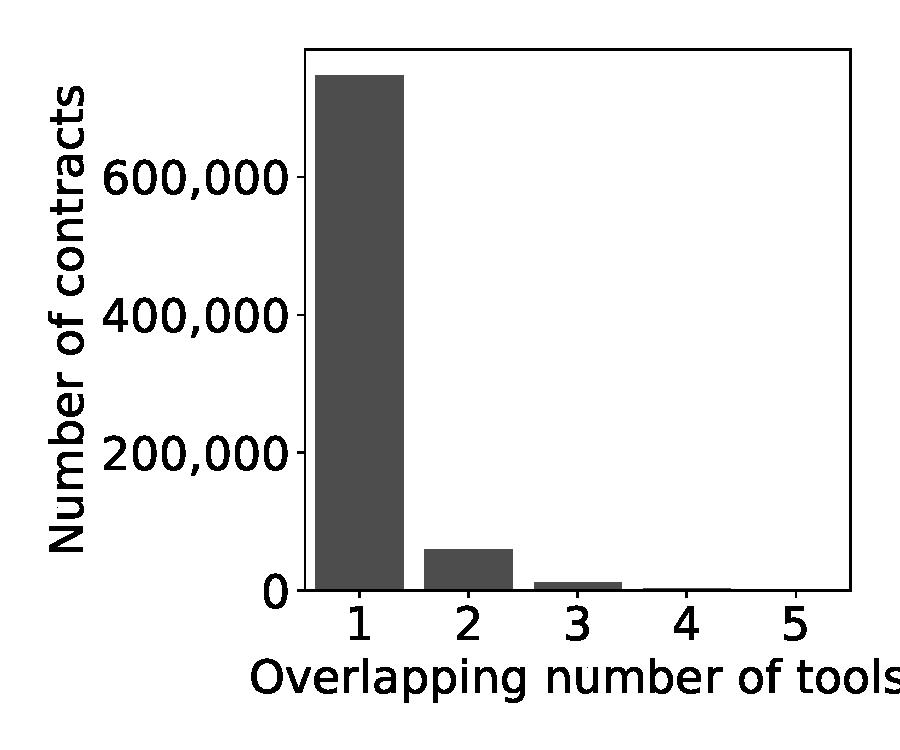
\includegraphics[width=\textwidth]{./5a-smart-contract-security/figures/overlap-analyzed.pdf}
    \caption{Overlapping contracts analysed.}
    \label{fig:all-overlap}
  \end{subfigure}
  \begin{subfigure}{0.48\columnwidth}
    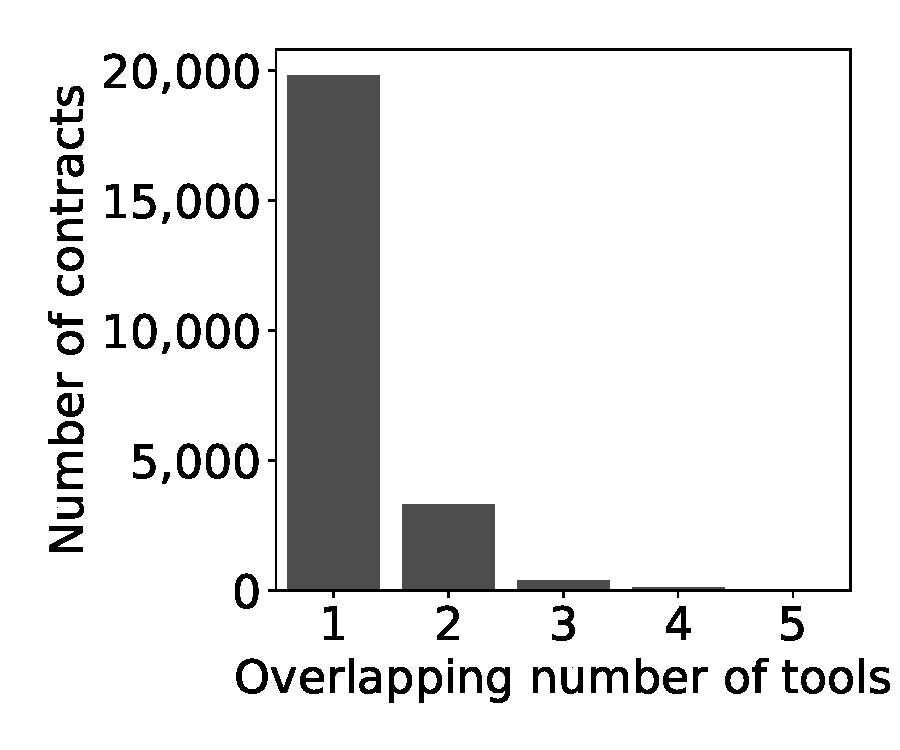
\includegraphics[width=\textwidth]{./5a-smart-contract-security/figures/overlap-vulnerable.pdf}
    \caption{Overlapping vulnerabilities flagged.}
    \label{fig:vulnerable-overlap}
  \end{subfigure}
  \caption[Overlap in the contracts analysed and flagged by examined tools]{Histograms that show the overlap in the contracts analysed and flagged by examined tools.}
\label{fig:hist-per-tool}
\end{figure}

\begin{table}[tb]
  \setlength{\tabcolsep}{2pt}
  \centering
  \caption{Agreement among tools for reentrancy analysis.}
  \label{fig:reentrancy-agreement}
  \begin{tabular}{lrrrr}
    \toprule
    \bf Tools & \bf Total & \bf Agreed & \bf Disagreed & \bf \% agreement\\
    \midrule
    Oyente/Securify & 774 & 185 & 589 & 23.9\%\\
    Oyente/Zeus & 104 & 3 & 101 & 2.88\%\\
    Zeus/Securify & 108 & 2 & 106 & 1.85\%\\
    \bottomrule
  \end{tabular}
\end{table}

\begin{table}
  \centering
  \setlength{\tabcolsep}{2pt}
  \small
  \caption{Mapping of the different vulnerabilities analyzed.}
  \label{fig:vuln-mapping}
  \begin{tabular}{lllllll}
    \toprule
    & \bf Oyente & \bf ZEUS & \bf Securify & \bf MadMax & \bf Maian & \bf teEther\\
    \midrule
    \bf \vre & reentrancy & reentrancy & no writes after call & --- & --- & ---\\
    \hline
    \bf \vue & callstack & unchecked send & handled exceptions & --- & --- & ---\\
    \hline
    \bf \vto & concurrency & tx order dependency & tx ordering dependency & --- & --- & ---\\
    \hline
    \bf \vle & --- & failed send & Ether liquidity & unbounded op & greedy & ---\\
    & & & & wallet griefing\\
    \hline
    \bf \vio & --- & integer overflow & --- & integer overflows & --- & --- \\
    \hline
    \bf \vua & --- & integer overflow & --- & integer overflows & prodigal & exploitable\\
    \bottomrule
  \end{tabular}
\end{table}

\point{Taxonomy}
Rather than reusing existing smart contract vulnerability taxonomies~\cite{atzei2017} as-is, we adapt it to fit the vulnerabilities analysed by the tools in our dataset.
We do not cover vulnerabilities not analyzed by at least \empirical{two} of the \PapersAnalyzed tools. We settle on the~\VulnTypes types of vulnerabilities described in \autoref{sec:5a:background}: reentrancy (\vre), unhandled exception (\vue), locked Ether (\vle), transaction order dependency (\vto), integer overflows (\vio) and unrestricted actions (\vua). As the papers we survey use different terms and slightly different definitions for each of these vulnerabilities, we map the relevant vulnerabilities to one of the \VulnTypes types of vulnerabilities we analyze. We show how we mapped these vulnerabilities in \autoref{fig:vuln-mapping}.

% \point{Excluded data}
% We exclude teEther~\cite{Krupp2018} and Maian~\cite{Nikolic2018a} from our analysis for two reasons. First, the amount of Ether at stake is too low to make an impact on our final results. The amount of Ether at stake for both tools combined represent a total of \empirical{14.89} Ether, which is \emph{six orders of magnitude} less than the total. Second, for the classes of vulnerabilities treated by these tools, it is almost impossible to assess if these vulnerabilities have been exploited or not. Indeed, for a vulnerability such as being able to destruct the contract, there is no general way of knowing if the person who performed such a call should have been allowed to do so. Given this lack of reliability and the very low amount of money at stake, we decided to keep this data out of further analysis.

\point{Overlapping vulnerabilities}
In this subsection, we first check how much overlap there is between contracts in our dataset: how many contracts have been analyzed by multiple tools and how many contracts were flagged vulnerable by multiple tools.
We note that most papers, except for~\cite{luu2016a}, are written around the same period.
We find that~\empirical{73,627} out of~\empirical{821,219} contracts have been analyzed by at least two of the tools but only~\empirical{13,751} by at least three tools.
In \autoref{fig:all-overlap}, we show a histogram of how many different tools analyze a single contract. In \autoref{fig:vulnerable-overlap}, we show the number of tools which flag a single contract as vulnerable to any of the analyzed vulnerabilities. The overlap for both the analyzed and the vulnerable contracts is relatively small. We assume one of the reasons is that some tools work on Solidity code~\cite{DBLP:conf/ndss/KalraGDS18} while other tools work on EVM bytecode~\cite{Tsankov2018,luu2016a}, making the population of contracts available different among tools.

We also find a lot of contradiction in the analysis of the different tools.
We choose reentrancy to illustrate this point, as it is supported by three of the tools we analyze. In \autoref{fig:reentrancy-agreement}, we show the agreement between the three tools supporting reentrancy detection. The \emph{Total} column shows the total number of contracts analyzed by both tools in the \emph{Tools} column and flagged by at least one of them as vulnerable to reentrancy. Oyente and Securify agree on only~\empirical{23\%} of the contracts, while Zeus does not seem to agree with any of the other tools.
This reflects the difficulty of building static analysis tools targeted at the EVM. While we are not trying to evaluate the different tools' performance, this gives us yet another motivation to find out the impact of the reported vulnerabilities.

\begin{lstlisting}[basicstyle=\footnotesize\ttfamily,language=json,float=tb,floatplacement=tb,caption=Sample execution trace information.,label=fig:execution-trace]
[
    {"op": "EQ", "pc": 7, 
    "depth": 1, "stack": ["2b", "a3"]},
    {"op": "ISZERO", "pc": 8, "depth": 1,
    "stack": ["00"]}
]
\end{lstlisting}

\subsection{Methodology}
\label{sec:methodology}

In this section, we describe in detail the different analyses we perform in order to check for exploits of the vulnerabilities described in \autoref{sec:5a:background}.

To check for potential exploits, we perform bytecode-level transaction analysis, whereby we look at the code executed by the contract when carrying out a particular transaction. We use this type of analysis to detect the~\VulnTypes types of vulnerabilities presented in \autoref{sec:5a:background}.

To perform our analyses, we first retrieve transaction data for all the contracts in our dataset. Next, to perform bytecode-level analysis, we extract the execution traces for the transactions which may have affected contracts of interest. We use the EVM's debug functionality, which gives us the ability to replay transactions and trace all the executed instructions. To speed up the data collection process, we patch the Go Ethereum client~\cite{go-ethereum}, as opposed to relying on the Remote Procedure Call~(RPC) functionality provided by the default Ethereum client.
We show a truncated sample of the extracted traces in \autoref{fig:execution-trace} for illustration. 
%
The \lstinline{op} key is the current instruction, \lstinline{pc} is the program counter, \lstinline{depth} is the current level of call nesting, and finally, \lstinline{stack} contains the current state of the stack. We use single-byte values in the example, but the actual values are 32 bytes (256 bits).

The extracted traces contain a list of executed instructions, as well as the state of the stack at each instruction.
To analyze the traces, we encode them into a Datalog representation; Datalog is a language implementing first-order logic with recursion~\cite{Immerman99descriptivecomplexity}, which allows us to concisely express properties about the execution traces.
We use the following domains to encode the information about the traces as Datalog facts, noting $V$ as the set of program variables and $A$ is the set of Ethereum addresses.
We show an overview of the facts that we collect and the relations that we use to check for possible exploits in Figure~\ref{fig:datalog-setup}.
We should highlight that our analyses run \emph{automatically} based on the facts that we extract and the rules that define various violations described in subsequent sections. 

\begin{figure}
  \centering
\begin{lstlisting}[language=Solidity,basicstyle=\footnotesize\ttfamily,label=fig:handled-exception-solidity,caption=Failure handling in Solidity.]
if (!addr.send(100)) { throw; }
\end{lstlisting}
\begin{lstlisting}[language=esm, basicstyle=\footnotesize\ttfamily,caption=EVM instructions for failure handling.,label=fig:handled-exception-instructions]
; preparing call
(0x65) CALL
; call result pushed on the stack
(0x69) PUSH1 0x73
(0x71) JUMPI ; jump to 0x73 if call was successful
(0x72) REVERT
(0x73) JUMPDEST
\end{lstlisting}
  \caption{Correctly handled failed \lstinline{send}.}
  \label{fig:handled-exception}
\end{figure}

% \point{Analysis correctness: effects of soundness and completeness}
% Soundness and completeness affect our results in the following ways: if the analysis is \emph{unsound}, we might be missing exploits and therefore \emph{underestimating} the amount of Ether exploited.
% On the other hand, if the analysis is \emph{incomplete}, we might be flagging as exploit benign transactions and \emph{overestimating} the amount exploited.
% One of our goals in this work is to provide an upper-bound of the total amount exploited.
% Therefore, if a choice needs to be made between these two properties, we choose soundness over completeness for our analysis.

% \begin{figure}[tb]
%   \setlength{\tabcolsep}{3pt}
% \begin{tabular}{lcc}
% \toprule
% &	\bf Sound	& \bf Complete \\
% \midrule
% Re-entrancy	                  & yes	& yes\\
% Unhandled exception	          & yes	& yes\\
% Locked ether	                & yes	& yes\\
% Transaction order dependency	& yes	& no\\
% Integer overflow	            & no\footnotemark	& no\\
% \bottomrule\\
% \end{tabular}
% \caption{Soundness and completeness properties for the analyses in this section.}
% \end{figure}

% \footnotetext{Section~\ref{ssec:method-io} and Section~\ref{ssec:analysis-io} provide in-depth explanations of the cases where the analysis is unsound}

%  is a set of statement identifiers;


\begin{figure}[tbp]
\begin{subfigure}[t]{\columnwidth}
  \centering
 \setlength{\tabcolsep}{4pt}
 %
 \footnotesize
\begin{tabular}{ll}
  \toprule
  \bf Fact &  \bf Description\\
  \midrule
  \dterm{is_output}{v_1\in V\dsep v_2\in V} & $v_1$ is an output of $v_2$\\
  \dterm{size}{v\in V \dsep n\in \mathbb{N}} & $v$ has $n$ bits\\
  \dterm{is_signed}{v\in V} & $v$ is signed\\
  \dterm{in_condition}{v\in V} & $v$ is used in a condition \\
  \dterm{call}{a_1\in A\dsep a_2\in A\dsep p\in \mathbb{N}} & $a_1$ calls $a_2$ with $p$ Ether\\
  \dterm{create}{a_1\in A\dsep a_2\in A\dsep p\in \mathbb{N}} & $a_1$ creates $a_2$ with $p$ Ether\\
  \dterm{expected_result}{v\in V\dsep r\in \mathbb{Z}} & $v$'s expected result is $r$\\
  \dterm{actual_result}{v\in V\dsep r\in \mathbb{Z}} & $v$'s actual result is $r$\\
  \multirow{2}{*}{\dterm{call_result}{v\in V\dsep n\in\mathbb{N}}} & $v$ is the result of a call\\
  & and has a value of $n$\\
  \multirow{2}{*}{\dterm{call_entry}{i\in \mathbb{N}\dsep a\in A}} & contract $a$ is called when\\
           & program counter is $i$\\
  \multirow{2}{*}{\dterm{call_exit}{i\in \mathbb{N}}} & program counter is $i$ when\\
           & exiting a call to a contract\\
  \multirow{2}{*}{\dterm{tx_sstore}{b\in \mathbb{N}, i\in \mathbb{N}, k\in \mathbb{N}}} & storage key $k$ is written in\\
  & transaction $i$ of block $b$\\
  \multirow{2}{*}{\dterm{tx_sload}{b\in \mathbb{N}, i\in \mathbb{N}, k\in \mathbb{N}}} & storage key $k$ is read in\\
  & transaction $i$ of block $b$\\
  \dterm{caller}{v\in V, a\in A} & $v$ is the caller with address $a$\\
  \dterm{load_data}{v\in V} & $v$ contains transaction call data\\
  \dterm{restricted_inst}{v\in V} & $v$ is used by a restricted instruction\\
  \dterm{selfdestruct}{v\in V} & $v$ is used in \op{SELFDESTRUCT}\\
  \bottomrule
\end{tabular}
\caption{Datalog facts.}
\label{fig:datalog-facts}
\end{subfigure}

\vspace{2mm}

\begin{subfigure}[t]{\columnwidth}
  \centering
  \setlength{\tabcolsep}{1pt}
  \footnotesize
\begin{tabular}{l}
  \toprule
  \bf Datalog rules\\
  \midrule
  \dterm{depends}{v_1\in V\dsep v_2\in V} \drulesep \dterm{is_output}{v_1\dsep v_2}\dend\\
  \dterm{depends}{v_1\dsep v_2} \drulesep \dterm{is_output}{v_1\dsep v_3}\dsep \dterm{depends}{v_3\dsep v_2}\dend\\
  \midrule
  \dterm{call_flow}{a_1\in A\dsep a_2\in A\dsep p\in \mathbb{Z}} \drulesep \dterm{call}{a_1\dsep a_2\dsep p}\dend\\
  \dterm{call_flow}{a_1\in A\dsep a_2\in A\dsep p\in \mathbb{Z}} \drulesep \dterm{create}{a_1\dsep a_2\dsep p}\dend\\
  \dterm{call_flow}{a_1\dsep a_2\dsep p} \drulesep \dterm{call}{a_1\dsep a_3\dsep p}\dsep
  \dterm{call_flow}{a_3\dsep a_2\dsep \_}\dend\\
  \midrule
  \dterm{inferred_size}{v\in V\dsep n\in \mathbb{N}}\drulesep \dterm{size}{v\dsep n}\dend\\
  \dterm{inferred_size}{v\dsep n}\drulesep \dterm{depends}{v\dsep v_2}\dsep \dterm{size}{v_2\dsep n}\dend\\
  \midrule
  \dterm{inferred_signed}{v\in V}\drulesep \dterm{is_signed}{v}\dend\\
  \dterm{inferred_signed}{v}\drulesep \dterm{depends}{v\dsep v_2}\dsep \dterm{is_signed}{v_2}\dend\\
  \midrule
  \dterm{condition_flow}{v\in V\dsep v\in V}\drulesep \dterm{in_condition}{v}\dend\\
  \dterm{condition_flow}{v_1\dsep v_2} \drulesep \dterm{depends}{v_1\dsep v_2}\dsep
  \dterm{in_condition}{v_2}.\\
  \midrule
  \dterm{depends_caller}{v\in V}\drulesep \dterm{caller}{v_2\dsep \_}\dsep \dterm{depends}{v, v_2}.\\
  \midrule
  \dterm{depends_data}{v\in V}\drulesep \dterm{load_data}{v_2\dsep \_}\dsep \dterm{depends}{v, v_2}.\\
  \midrule
  \dterm{caller_checked}{v \in V}\drulesep \dterm{caller}{v_2, \_}\dsep\\
  \hspace{11.7em}\dterm{condition_flow}{v_2, v_3}\dsep $v_3 < v$.\\
  \bottomrule
\end{tabular}
\caption{Datalog rule definitions.}
\label{fig:relations}
\end{subfigure}

\vspace{2mm}

\begin{subfigure}[t]{\columnwidth}
  \centering
  \footnotesize
  \setlength{\tabcolsep}{1pt}
  \begin{tabular}{ll}
    \toprule
    \bf Vulnerability & \bf Query \\
    \midrule
    \reentrancy & \dterm{call_flow}{a_1\dsep a_2\dsep p_1}\dsep \\
                      & \dterm{call_flow}{a_2\dsep a_1\dsep p_2}\dsep $a_1 \neq a_2$\\
    \midrule
    Unhandled Excep. & \dterm{call_result}{v\dsep 0}\dsep $\lnot$\dterm{condition_flow}{v, \_}\\
    \midrule
    Transaction Order & \dterm{tx_sstore}{b, t_1, i}\dsep \\
    Dependency & \dterm{tx_sload}{b, t_2, i}, $t_1 \neq t_2$\\
    \midrule
    \lockedether & \dterm{call_entry}{i_1, a}\dsep \dterm{call_exit}{i_2}, $i_1 + 1 = i_2$\\
    \midrule
    \integeroverflow & \dterm{actual_result}{v\dsep r_1}\dsep\\
                              & \dterm{expected_result}{v\dsep r_2}\dsep$r_1 \neq r_2$\\
    \midrule
    \unrestrictedaction & \dterm{restricted_inst}{v}\dsep \dterm{depends_data}{v}\dsep\\
                      & $\lnot$\dterm{depends_caller}{v}\dsep $\lnot$\dterm{caller_checked}{v}\\
    & $\lor$ \dterm{selfdestruct}{v}\dsep $\lnot$\dterm{caller_checked}{v}\\
    \bottomrule
  \end{tabular}
  \caption{Datalog queries for detecting different vulnerability classes.}
\label{fig:queries}
\end{subfigure}
\caption{Datalog setup.}
\label{fig:datalog-setup}
\end{figure}


\subsubsection{\reentrancy}
In the EVM, as transactions are executed independently, re-entrancy issues can only occur \emph{within} a single transaction. Therefore, for re-entrancy to be exploited, there must be a call to an external contract which invokes, directly or indirectly, a re-entrant callback to the calling contract. We therefore start by looking for \op{CALL} instructions in the execution traces, while keeping track of the contract currently being executed.

When \op{CALL} is executed, the address of the contract to be called as well as the value to be sent can be retrieved by inspecting the values on the stack~\cite{wood2014ethereum}. Using this information, we can record \dterm{call}{a_1,a_2,p} facts described in Figure~\ref{fig:datalog-facts}.
We note that a contract can also create a new contract using \op{CREATE} and execute a re-entrancy attack using it~\cite{Rodler2019}. We therefore treat this instruction in a similar way as \op{CALL}.
Using these, we then use the query shown in Figure~\ref{fig:queries} to retrieve potentially malicious re-entrant calls.

\correctness Our analysis for re-entrant calls is sound but not complete. As the EVM executes each contract in a single thread, a re-entrant call must come from a recursive call. For example, given $A$, $B$, $C$ and $D$ being functions, a re-entrant call could be generated with a call path such as $A\rightarrow B \rightarrow C\rightarrow A$. Our tool searches for all mutually-recursive calls; it supports an arbitrarily-long calls path by using a recursive Datalog rule, making the analysis sound. However, we have no way of assessing if a re-entrant call is malicious or not, which can lead to false positives.

\subsubsection{\unhandledexceptions}
%
When Solidity compiles contracts, methods to send Ether, such as \lstinline{send}, are compiled into the EVM \op{CALL} instructions. We show an example of such a call and its instructions counterpart in \autoref{fig:handled-exception-instructions}. If the address passed to \op{CALL} is an address, the EVM executes the code of the contract, otherwise it executes the necessary instructions to transfer Ether to the address. When the EVM is done executing, it pushes either $1$ on the stack, if the \op{CALL} succeeded, or $0$ otherwise. 

To retrieve information about call results, we can therefore check for \op{CALL} instructions and use the value pushed on the stack after the call execution. The end of the call execution can be easily found by checking when the \lstinline{depth} of the trace turns back to the value it had when the \op{CALL} instruction was executed; we save this information as \dterm{call_result}{v\dsep n} facts.
An important edge case to consider are calls to pre-compiled contracts, which are typically called by the compiler and do not require their return value to be checked, as they are results to computation where $0$ could be a valid value, but could result in false-positives.
As pre-compiled contracts have known addresses between 1 and 10, we choose to simply not record \lstinline{call_result} facts for such calls.

As shown in Figure~\ref{fig:handled-exception-instructions}, the EVM uses the \op{JUMPI} instruction to perform conditional jumps. At the time of writing, this is the only instruction available to execute conditional control flow. We therefore mark all the values used as a condition in \op{JUMPI} as \lstinline{in_condition}. We can then check for the unhandled exceptions by looking for call results, which never influence a condition using the query shown in Figure~\ref{fig:queries}.

\correctness The analysis we perform to check for unhandled exceptions is complete but not sound.
All failed calls in the execution of the program will be recorded, while we accumulate facts about the execution.
We then use a recursive Datalog rule to check if the call result is used directly or indirectly in a condition.
We could obtain false negatives if the call result is used in a condition but the condition is not enough to prevent an exploit.
However, given that the most prevalent pattern for this vulnerability is the result of \lstinline{send} not being used at all~\cite{Tsankov2018}, and when the result is used, it is typically done within a \lstinline{require} or \lstinline{assert} expression, we hypothesize that such false negatives should be very rare.

\subsubsection{\lockedether}
Although there are several reasons for funds locked in a contract, we focus on the case where the contract relies on an external contract which does not exist anymore, as this is the pattern which had the largest financial impact on Ethereum~\cite{Breidenbach}. Such a case can occur when a contract uses another contract as a library to perform some actions on its behalf. To use a contract in this way, the \op{DELEGATECALL} instruction is used instead of \op{CALL}, as the latter does not preserve call data, such as the sender or the value.

The next important part is the behavior of the EVM when trying to call a contract which does not exist anymore.
When a contract is destructed, it is not completely removed per-se, but its code is not accessible anymore to callers.
When a contract tries to call a contract which has been destructed, the call is a no-op rather than a failure, which means that the next instruction will be executed and the call will be marked as successful.
To find such patterns, we collect Datalog facts about all the values of the program counter before and after every \lstinline{DELEGATECALL} instruction. In particular, we first mark the program counter value at which the call is executed~---~\dterm{call_entry}{i_1\in \mathbb{N}\dsep a\in A}. Then, using the same approach as for unhandled exceptions, we skip the content of the call and mark the program counter value at which the call returns~---~\dterm{call_exit}{i_2\in \mathbb{N}}.

If the called contract does not exist anymore, $i_1 + 1 = i_2$ must hold. Therefore, we can use the Datalog query shown in Figure~\ref{fig:queries} to retrieve the destructed contracts address.

\correctness The approach we use to detect locked Ether is sound and complete for the class of locked funds vulnerability we focus on. All vulnerable contracts must have a \lstinline{DELEGATECALL} instruction. If the issue is present and the call contract has indeed been destructed, it will always result in a no-op call. Our analysis records all of these calls and systematically check for the program counter before and after the execution, making the analysis sound and complete.


\subsubsection{\transactionorder}
The first insight to check for exploitation of transaction ordering dependency is that at least two transactions to the same contract must be included in the same block for such an attack to be successful. Furthermore, as shown in~\cite{Luu2016a} or~\cite{Tsankov2018}, exploiting a transaction ordering dependency vulnerability requires manipulation of the contract's storage.

The EVM has only one instruction to read from the storage, \op{SLOAD}, and one instruction to write to the storage, \op{SSTORE}. In the EVM, the location of the storage to use for both of these instructions is passed as an argument, and referred to as the storage \emph{key}. This key is available on the stack at the time the instruction is called. We go through all the transactions of the contracts and each time we encounter one of these instructions, we record either~\dterm{tx_sload}{b\in \mathbb{N}, i\in \mathbb{N}, k\in \mathbb{N}} or \dterm{tx_sstore}{b\in \mathbb{N}, i\in \mathbb{N}, k\in \mathbb{N}} where in each case $b$ is the block number, $i$ is the index of the transaction in the block and $k$ is the storage key being accessed.

The essence of the rule to check for transaction order dependency issues is then to look for patterns where at least two transactions are included in the same block with one of the transactions writing a key in the storage and another transaction reading the same key. We show the actual rule in Figure~\ref{fig:queries}.

\correctness Our approach to check for transaction order dependencies is sound but not complete. With the definition we use, for a contract to have a transaction order dependency it must have two transactions in the same block, which affect the same key in the storage. We check for all such cases, and therefore no false-negatives can exist. However, finding if there is a transaction order dependency requires more knowledge about how the storage is used and our approach could therefore result in false positives.


\subsubsection{\integeroverflow}
\label{ssec:method-io}

% \begin{figure}[tb]
%   \centering
%   \setlength{\tabcolsep}{14pt}
%   \begin{tabular}{rl}
%     \toprule
%     \textbf{Instruction} & \textbf{Description}\\
%     \midrule
%     \op{SIGNEXTEND} & Increase the number of bits\\
%     \op{SLT} & Signed lower than\\
%     \op{SGT} & Signed greater than\\
%     \op{SDIV} & Signed division\\
%     \op{SMOD} & Signed modulo\\
%     \bottomrule
%   \end{tabular}
%   \caption{EVM instructions that operate on signed operands.}
%   \label{fig:signed-instructions}
% \end{figure}
%
The EVM is completely untyped and expresses everything in terms of~256-bits words. Therefore, types are handled entirely at the compilation level and there is no explicit information about the original types in any execution traces.

To check for integer overflow, we accumulate facts over two passes. In the first pass, we try to recover the sign and size of the different values on the stack. To do so, we use known invariants about the Solidity compilation process. First, any value which is the result of an instruction such as \op{SIGNEXTEND} or \op{SDIV} can be marked to be signed with \dterm{is_signed}{v}. Furthermore, \op{SIGNEXTEND} being the usual sign extension operation for two's complement, it is passed both the value to extend and the number of bits of the value. This allows to retrieve the size of the signed value. We assume any value not explicitly marked as signed to be unsigned. To retrieve the size of unsigned values, we use another behavior of the Solidity compiler. 

To work around the lack of type in the EVM, the Solidity compiler inserts an \op{AND} instruction to ``cast'' unsigned integers to their correct value. For example, to emulate an \lstinline{uint8}, the compiler inserts \lstinline{AND value 0xff}. In the case of a ``cast'', the second operand $m$ will always be of the form $m = 16^n - 1,~n\in \mathbb{N},~n = 2^p,~p \in [1, 6]$. We use this observation to mark values with the according type: \lstinline{uintN} where $N = n \times 4$. Variables size are stored as \dterm{size}{v\dsep n} facts.

During the second phase, we use the \dterm{inferred_signed}{v} and \dterm{inferred_size}{v\dsep n} rules shown in Figure~\ref{fig:relations} to retrieve information about the current variable. When no information about the size can be inferred, we over-approximate it to $256$ bits, the size of an EVM word. Using this information, we compute the expected value for all arithmetic instructions (e.g. \op{ADD}, \op{MUL}), as well as the actual result computed by the EVM and store them as Datalog facts. Finally, we use the query shown in Figure~\ref{fig:queries} to find instructions which overflow.

\correctness Our analysis for integer overflow is neither sound nor complete. The types are inferred by using properties of the compiler using a heuristic which should work for most of cases but can fail. For example, if a contract contains code which yields \lstinline{AND value 0xff} but value is an \lstinline{uint32}, our type inference algorithm would wrongly infer that this variable is an \lstinline{uint8}. Such error during type inference could cause both false positives and false negatives. However, this type of issue occurs only when the developer uses bit manipulation with a mask similar to what the Solidity compiler generate. We find that such a pattern is rare enough not to skew our data, and give an estimate the possible number of contracts which could follow such a pattern in Section~\ref{ssec:analysis-io}.

\subsubsection{\unrestrictedaction}
\label{ssec:method-ua}
Unrestricted actions is a broad class of vulnerability, as it can include the ability to set an owner without being allowed to, destruct a contract without permission or yet execute arbitrary code.
As one of our main goal is to check the exploitation of vulnerable contracts, we stay close to the definitions given by previous works~\cite{Krupp2018} and focus on unrestricted Ether transfer using \op{CALL}, unrestricted writes using and \op{SSTORE}, and code injection using \op{DELEGATECALL} or \op{CALLCODE}.

First, we need to remind ourselves that the caller, unlike for example the call data, cannot be forged.
Therefore, one of the main insight is that if an action is restricted depending on who is calling, there should be an execution trace before the restricted operation which conditionally jumps, depending on the caller.
This is enough for \op{SELFDESTRUCT} but not for other instructions as it would flag a line such as \lstinline{balances[msg.sender] = msg.value} to be vulnerable.
To model this, we track whether the message sender influences the storage key or the address to call.
Finally, for code injection, we check whether the passed data influences the address called by \op{DELEGATECALL} or \op{CALLCODE}.

\correctness Our analysis for unrestricted actions is neither sound nor complete.
We take a relatively simple approach of checking whether the message sender influences a condition or not before executing a sensitive instruction.
This can result in false negatives because the check could be performed inappropriately, for example not reverting the transaction when needed, making the analysis unsound.
Furthermore, there might be some use cases where it is acceptable to allow any sender to write to the storage, but our analysis would flag such as vulnerable, resulting in false positives.
We discuss the implications further in Section~\ref{ssec:analysis-ua}.

\begin{figure}[tb]
  \centering
\small
\setlength{\tabcolsep}{2pt}
\begin{tabular}{llr}
\toprule
\bf Contract address & \bf Last & \bf Amount \\
 & \bf transaction & \bf exploited \\
\midrule
\addr[\scriptsize]{0xd654bdd32fc99471455e86c2e7f7d7b6437e9179} & 2016-06-10 & 5,885\\
\addr[\scriptsize]{0x675e2c143295b8683b5aed421329c4df85f91b33} & 2015-12-31 & 50.49\\
\addr[\scriptsize]{0xcd3e727275bc2f511822dc9a26bd7b0bbf161784} & 2017-03-25 & 10.34\\
\bottomrule
\end{tabular}
\caption{\vre: Top contracts victim of re-entrancy attack and ETH amounts exploited}
\label{fig:reentrancy-vulnerable}
\end{figure}



\subsection{Analysis of Individual Vulnerabilities}
\label{sec:5a:analysis}

As described in \autoref{sec:5a:datasets}, the combined amount of Ether contained within \emph{all} the vulnerable contracts exceeds~\empirical{3 million} ETH, worth~\empirical{\numprint{\ToUSD{3}} million} USD. In this section, we present the results for each vulnerability one by one; our results have been obtained using the methodology described in \autoref{sec:5a:methodology}; the goal is to show how much of this money is actually at risk.

\point{Methodology}
For each vulnerability, we perform our analysis in two steps.
First, we fetch the execution traces of all the transactions up to block~\block{10200000} affecting the contracts in our dataset, either directly or through internal transactions. We then run our tool to automatically find the total amount of Ether at risk and report this number.
This is the amount we use to later give a total upper bound across all vulnerabilities.
In the second step, we manually analyze the contracts at risk to obtain more insight into the exploits and find interesting patterns.
As analysing all the contracts manually would be impractical, for each vulnerability we manually analyze the contracts with the highest amount of Ether at risk to understand better the reasons behind the vulnerabilities.
We then present interesting findings as short case studies.

\point{Runtime performance} Our analysis runs in linear time and memory with respect to the number of instructions executed by a given transaction. The number of instructions varies widely between transactions, anywhere from a few hundred to a few hundred thousand, with an average of around \empirical{100,000}. Our tool takes on average less than \empirical{10}ms (stddev. \empirical{20}ms) per transaction with a maximum of less than \empirical{2} seconds for the largest transactions, which is below the timeout of \empirical{5} seconds which we set for a single transaction.

% report all the contracts with a potential amount of Ether at risk greater than 10 ETH. We choose 10 ETH as a threshold because we think it is low enough to not miss any important attack while being high enough to filter out most of the contracts. It is therefore appropriate for manual inspection efforts. It is important to note that the filter used in this step affects in no way the total amount we report, and is used purely for practical purposes.

\subsubsection{\vre: \reentrancy}
\label{ssec:analysis-re}
There are~\empirical{4,337} contracts flagged as vulnerable to reentrancy by~\cite{luu2016a,Tsankov2018,DBLP:conf/ndss/KalraGDS18}, with a total of~\empirical{457,073} transactions. After running the analysis described in \autoref{sec:5a:methodology} on all the transactions, we found a total of~\empirical{116} contracts which contain re-entrant calls. To look for the monetary amount at risk, we compute the sum of the Ether sent between two contracts in transactions containing re-entrant calls. The total amount of Ether exploited using reentrancy is of~\empirical{6,076 ETH}, which is considerable, as it represents more than \empirical{\numprint{\ToUSD{6000}} USD}.

\point{Manual analysis}
We manually analyze the top contracts in terms of funds lost and present them in \autoref{fig:reentrancy-vulnerable}. Interestingly, one of these~\empirical{three} potential exploits has a substantial amount of Ether at stake:~\empirical{5,881 ETH}, which corresponds to around~\empirical{\numprint{\ToUSD{5900}} USD}. This address has already been detected as vulnerable by some recent work focusing on reentrancy~\cite{Rodler2019}. It appears that the contract, which is part of the Maker DAO~\cite{maker-dao} platform, was found vulnerable by the authors of the contract, who themselves performed an attack to confirm the risk~\cite{ds-eth-token}.

\point{Sanity checking}
We use two different contracts for sanity checking.
First, we look at TheDAO attack, which is the most famous instance of a reentrancy attack. Our tool detects the following reentrancy pattern: \href{https://etherscan.io/address/0xc0ee9db1a9e07ca63e4ff0d5fb6f86bf68d47b89}{the malicious account} calls \href{https://etherscan.io/address/0xbb9bc244d798123fde783fcc1c72d3bb8c189413}{TheDAO main account}, TheDAO main account calls into \href{https://etherscan.io/address/0xd2e16a20dd7b1ae54fb0312209784478d069c7b0}{the reward account} and the reward account sends the reward to the malicious account, allowing it to perform the re-entrant call into TheDAO main account.

As another sanity check, we look at a contract called SpankChain~\cite{spank-chain}, which is known to recently have been compromised by a reentrancy attack. We confirm that our approach successfully marks this contract as having been the victim of a reentrancy attack and correctly identifies the attacker contract.

Finally, we note that our tool finds all the reentrancy patterns presented by Sereum~\cite{Rodler2019}, including delegated and create-based reentrancy\footnote{https://github.com/uni-due-syssec/eth-reentrancy-attack-patterns}.

\begin{figure}[tb]
  \centering
\small
\begin{tabular}{lr}
\toprule
\bf Contract address & \bf Amount at risk\\
\midrule
\addr[\scriptsize]{0x7011f3edc7fa43c81440f9f43a6458174113b162} & 56.70\\
\addr[\scriptsize]{0xb336a86e2feb1e87a328fcb7dd4d04de3df254d0} & 42.27\\
\addr[\scriptsize]{0xdcabd383a7c497069d0804070e4ba70ab6ecdd51} & 33.44\\
\addr[\scriptsize]{0xfd2487cc0e5dce97f08be1bc8ef1dce8d5988b4d} & 21.60\\
\addr[\scriptsize]{0x9e15f66b34edc3262796ef5e4d27139c931223f0} & 10.50\\
\bottomrule
\end{tabular}
\caption{\vue: Top contracts affected by unhandled exceptions and ETH amounts at risk}
\label{fig:unhandled-exceptions}
\end{figure}


\subsubsection{\vue: \unhandledexceptions}
\label{ssec:analysis-ue}
There are \empirical{11,427} contracts flagged vulnerable to unhandled exceptions by~\cite{Tsankov2018,luu2016a,DBLP:conf/ndss/KalraGDS18} for a total of more than~\empirical{3.4 million} transactions, which is \emph{an order of magnitude} larger than what we found for reentrancy issues.

We find a total of~\empirical{264} contracts where failed calls have not been checked for, which represents roughly~\empirical{2\%} of the flagged contracts. The next goal is to find an upper bound on the amount of Ether at risk because of these unhandled exceptions. We define the upper bound on the money at risk to be the minimum value of the balance of the contract at the time of the unhandled exception and the total of Ether which have failed to be sent. We then sum the upper bound of all issues found to obtain a total upper bound. This gives us a total of \empirical{271.89} Ether at risk for unhandled exceptions.

\point{Manual analysis}
We manually analyze the top contracts and summarize their addresses and the amount at risk in \autoref{fig:unhandled-exceptions}. The Solidity code is available for \empirical{three} of these contracts. We confirm that in all cases the issue came from misuse of a low-level Solidity function such as \lstinline{send}.

\begin{investigation}{0x7011f3edc7fa43c81440f9f43a6458174113b162}
	The contract {\small\addr{0x7011f3edc7fa43c81440f9f43a6458174113b162}} has failed to send a total of \empirical{52.90} Ether and currently still holds a balance of \empirical{69.3} Ether at the time of writing. After investigation, we find that the contract is an abandoned pyramid scheme~\cite{ethereum-pyramid}. The contract has a total of \empirical{21} calls which failed, all trying to send \empirical{2.7} Ether, which appears to have been the reward of the pyramid scheme at this point in time. Unfortunately, the code of this contract was not available for further inspection but we conclude that there is a high chance that some of the users in the pyramid scheme did not correctly obtain their reward because of this issue.
\end{investigation}


% \begin{figure}[tb]
  \centering
\small
\setlength{\tabcolsep}{2pt}
\begin{tabular}{llr}
\toprule
\bf Contract address & \bf  Last send  & \bf Balance \\
\midrule
\addr[\scriptsize]{0x7da82c7ab4771ff031b66538d2fb9b0b047f6cf9} &  2017-11-15 &     369,023 \\
\addr[\scriptsize]{0x4a412fe6e60949016457897f9170bb00078b89a3} &  2018-01-25 &     4,000 \\
\addr[\scriptsize]{0x90420b8aef42f856a0afb4ffbfaa57405fb190f3} &  2018-01-08 &     636.7 \\
\addr[\scriptsize]{0x49edf201c1e139282643d5e7c6fb0c7219ad1db7} &  2017-05-20 &     44.23 \\
\addr[\scriptsize]{0x40a05d4ce308bf600cb275d7a3e9113518f59c54} &  2017-09-11 &     39.48 \\
\bottomrule
\end{tabular}
    \caption[\textsf{LE}: Top inactive contracts flagged with locked Ether funds]{\textsf{LE}: Top inactive contracts flagged with locked Ether funds (The send date is \emph{from} the contract).}
    \label{fig:dependency}
\end{figure}


\subsubsection{\vle: \lockedether}
\label{ssec:analysis-le}
There are~\empirical{7,285} contracts flagged vulnerable to locked Ether by~\cite{Tsankov2018},~\cite{Grech2018},~\cite{Nikolic2018a} and~\cite{DBLP:conf/ndss/KalraGDS18}. The contracts hold a total value of more than~\empirical{1.4 million} ETH, which is worth more than \empirical{\numprint{\ToUSD{1}} million USD}. We analyze the transactions of the contracts that could potentially be locked by conducting the analysis described in the previous section. Our tool shows that \emph{none} of the contracts are affected by the pattern we check for~---~i.e., dependency on a contract that had been destructed.
We note that our tool currently only covers dependency on a destructed contract as a reason for locked Ether and patterns such as unbounded mass operation are not yet covered.

\point{Parity wallet}
Contracts affected by the Parity wallet \footnote{Parity wallet Address: \addr{0x863df6bfa4469f3ead0be8f9f2aae51c91a907b4}} bug \cite{Breidenbach}, which our tool should flag as locked Ether, were not flagged by the tools we analysed, and are therefore not present in our dataset.
As this is one of the most famous cases of locked Ether, we test our tooling on the contracts affected by the Parity wallet bug.
To find the contracts, we simply have to use the Datalog query for locked Ether in \autoref{fig:queries} and insert the value of the Parity wallet address as argument $a$. Our results for contracts affected by the Parity bug indeed match what others had found in the past~\cite{parity-wallet-freeze}, with the contract at address~\addr{0x3bfc20f0b9afcace800d73d2191166ff16540258} having as much as \empirical{306,276 ETH} locked.

% \point{Transaction pattern analysis}
% It is worth pointing out that some tools, such as MadMax~\cite{Grech2018},  check for other types of issues, which could also lock Ether. To try to check for such issues ourselves, we search for contracts with high monetary value, which have been inactive for a notably long period to see whether Ether is indeed locked.

% We find a total of~\empirical{15} contracts, which follow this pattern. We show the~\empirical{5} contracts with the highest balance in \autoref{fig:dependency}. We manually inspect the top \empirical{three} contracts, which contain a substantial amount of Ether, as well as the contracts, which have never \emph{sent} any Ether. These top three contracts are all implementing multi-sig wallets, which are typically used to store Ether for long periods, thus explaining the inactivity. After further manual inspection, we concluded that none of the contracts had been exploited, nor were exploitable.

% The first contract, which never sent any Ether, at address \addr{0x5a5eff38da95b0d58b6c616f2699168b480953c9} has its code publicly available. After inspection, it seems to be a ``lifelog'' and the fact it is not sending Ether seems to be there by design; in other words, the funds are not locked. Although we were not able to inspect the other contract because its code was not available, we did not find any vulnerability report for this address.


\begin{figure}[tb]
  \centering
\small
\setlength{\tabcolsep}{2pt}
\begin{tabular}{llr}
\toprule
\bf Contract address & \bf First issue & \bf Balance \\
\midrule
\addr[\scriptsize]{0x3da71558a40f63b960196cc0679847ff50fad22b} & 2016-09-06 & 13,818\\
\addr[\scriptsize]{0xd79b4c6791784184e2755b2fc1659eaab0f80456} & 2016-05-03 & 2,013\\
\addr[\scriptsize]{0xf45717552f12ef7cb65e95476f217ea008167ae3} & 2016-03-15 & 1,064\\
\bottomrule
\end{tabular}
\caption{\textsf{TOD}: Top contracts potentially victim of transaction ordering dependency attack.}
\label{fig:tod-vulnerable}
\end{figure}


\subsubsection{\vto: \transactionorder}
There are~\empirical{1,881} contracts flagged vulnerable to transaction ordering dependency by~\cite{luu2016a} and~\cite{DBLP:conf/ndss/KalraGDS18}. We run the analysis described in \autoref{sec:5a:methodology} on their \empirical{3,002,304} transactions and obtain a total of~\empirical{54} contracts potentially affected by transaction-order dependency. To estimate the amount of Ether at risk, we sum up the total value of Ether sent, including by internal transactions, during all the flagged transactions, resulting in a total of~\empirical{297.2 ETH} at risk of transaction-order dependency.

\point{Manual analysis}
For each contract, we find the block where transaction order dependency could have happened with the highest balance and report top with their balance at the time of the issue in \autoref{fig:tod-vulnerable}. We manually investigated the contracts listed, they all had their source code available. We confirmed that in all the contracts, a user could read and write to the same storage location within a single block. We inspected further \addr{0x3da71558a40f63b960196cc0679847ff50fad22b}, a contract called \lstinline{WithDrawChildDAO} and found that the read was simply for users to check their balance, making the issue benign.

% \begin{figure}[tb]
  \centering
\small
\setlength{\tabcolsep}{3pt}
\begin{tabular}{llr}
\toprule
\bf Contract address & \bf First issue & \bf Balance\\
\midrule
\addr[\scriptsize]{0x2935aa0a2d2fbb791622c29eb1c117b65b7a9085} & 2015-10-08 & 3,197\\
\addr[\scriptsize]{0x709c7134053510fce03b464982eab6e3d89728a5} & 2016-12-20 & 195.6\\
\addr[\scriptsize]{0x6dfaa563d04a77aff4c4ad2b17cf4c64d2983dc8} & 2016-06-24 & 178.6\\
\addr[\scriptsize]{0x0096800019bf4eca0bed5a714a553ecf844884c5} & 2016-06-21 & 174.0\\
\addr[\scriptsize]{0x9f53cdb4ea5b205a2fcd079f54af7196b1288938} & 2016-06-29 & 106.5\\
\bottomrule
\end{tabular}
\caption{\textsf{IO}: Top contracts potentially victim of integer overflows.}
\label{fig:integer-overflow}
\end{figure}


\begin{table}[tb]
	\centering
	\caption{Understanding the exploitation of potentially vulnerable contracts.}
	\label{fig:findings-summary}
	\small
	\setlength{\tabcolsep}{1pt}
	\begin{tabular}{|lrrr||rr||rr|}
		\hline

		\multicolumn{4}{|c||}{\bf Vulnerable} & \multicolumn{2}{c||}{\bf Exploited contracts} &
		\multicolumn{2}{c|}{\bf Exploited Ether}                                                                                                                                                                                                      \\ \hline
		\bf Vuln.                             & \bf Vuln.                                     & \bf Total Ether & \bf Transactions         & \bf Contracts          & \bf \% of contracts        & \bf Exploited   & \bf \% of Ether \bigstrut[t]     \\
		                                      & \bf contracts                                 & \bf at stake    & \bf analysed             & \bf exploited          & \bf exploited              & \bf Ether       & \bf exploited                    \\

		\hline\hline
		\vre                                  & 4,337                                         & 1,518,067       & 457,073                  & 116                    & 2.68\%                     & 6,076           & 0.40\% \bigstrut[t]              \\
		\vue                                  & 11,427                                        & 419,418         & 3,400,960                & 264                    & 2.31\%                     & 271.9           & 0.068\%                          \\
		\vle                                  & 7,285                                         & 1,416,086       & 10,660,066               & 0                      & 0\%                        & 0               & 0\%                              \\
		\vto                                  & 1,881                                         & 302,679         & 3,002,304                & 54                     & 3.72\%                     & 297.2           & 0.091\%                          \\
		\vio                                  & 2,492                                         & 602,980         & 1,295,913                & 62                     & 2.49\%                     & 1,842           & 0.31\%                           \\
		\vua                                  & 5,163                                         & 580,927         & 3,871,770                & 42                     & 0.813\%                    & 0               & 0\%                              \\
		\hline
		\bf Total                             & \VulnerableContracts                          & \EtherStake     & \NumAnalyzedTransactions & \NumExploitedContracts & \PercentExploitedContracts & \ExploitedEther & \PercentExploitedEther \bigstrut \\
		\hline
	\end{tabular}
\end{table}


\subsubsection{\vio: \integeroverflow}
\label{ssec:analysis-io}
There are \empirical{2,472} contracts flagged vulnerable to integer overflow, which accounts for a total of more than~\empirical{1.2 million transactions}. We run the approach we described in \autoref{sec:5a:methodology} to search for actual occurrences of integer overflows.
It is worth noting that for integer overflow analysis we rely on the properties of the Solidity compiler. To ensure that the contracts we analyze were compiled using Solidity, we fetched all the available source codes for contracts flagged vulnerable to integer overflow from Etherscan~\cite{etherscan}. Out of~\empirical{2,492} contracts,~\empirical{945} had their source code available and all of them were written in Solidity.

\point{Effects of our formulation}
As mentioned in \autoref{ssec:method-io}, some types of bit manipulation in Solidity contracts could result in our type inference heuristic failing. We use the source codes we collected here to verify to what extent this could affect our analysis. We find that bit manipulation by itself is already fairly rare in Solidity, with only~\empirical{244} out of the~\empirical{2,492} contracts we collected using any sort of bit manipulation. Furthermore, most of the contracts using bit manipulation were using it to manipulate a variable as a bit array, and only ever retrieved a single bit at a time. Such a pattern does not affect our analysis. We found only~\empirical{33} contracts which used \lstinline{0xFF} or similar values, which could actually affect our analysis. This represents about \empirical{1.3\%} of the number of contracts for which the source code was available.

We find a total of~\empirical{62} contracts with transactions where an integer overflow might have occurred.
To find the amount of Ether at stake, we analyze all the transactions which resulted in integer overflows. We approximate the amount by summing the total amount of Ether transferred in and out during a transaction containing an overflow. We find that the total Ether at stake is~\empirical{1,842 ETH}. This is most likely an over-approximation but we use this value as our upper bound.

\point{Manual analysis}
We inspect some of the results we obtained a little further to get a better sense of what kind of cases lead to overflows.
We find that a very frequent cause of overflow is rather an underflow of unsigned values.
We highlight one such case in the following investigation.

\begin{investigation}{0xdcabd383a7c497069d0804070e4ba70ab6ecdd51}
	This contract was flagged positive to both unhandled exceptions and integer overflow by our tool.
	%
	After inspection, it seems that at block height~\block{1364860}, the owner tried to reduce the fees but the unsigned value of the fees overflowed and became a huge number. Because of this issue, the contract was then trying to send large amounts of Ether.
	%
	This resulted in failed calls which happened not to be checked, hence the flag for unhandled exceptions.
\end{investigation}

\subsubsection{\unrestrictedaction}
\label{ssec:analysis-ua}
There is a total of \empirical{5,163} contracts flagged by~\cite{Tsankov2018,Nikolic2018a,Krupp2018} as vulnerable to unrestricted actions for a total of \empirical{3,871,770} transactions. We use the approach described in \autoref{ssec:method-ua} and find a total of \empirical{42} contracts having suffered unrestricted actions, which were all non-restricted self-destructs, but none of them held Ether at the time of the exploit.

\point{Effects of our formulation} As mentioned in \autoref{ssec:method-ua}, this analysis is not sound, which means we need to be cautious about false positives.
A contract could have a check on the message sender which is incorrect and be exploited but not be flagged as such.
While we hypothesize that it is an edge case, it cannot be completely excluded.
However, having an automation method for such a check requires knowing the intent of the programmer, for example through specifications, which is out-of-scope of this work.
Therefore, we decide to inspect the contracts in our dataset in more detail to understand better the level of exploitation.

\point{Manual analysis}
The tool teEther flags \emph{exploitable} contracts, as opposed to simply \emph{vulnerable} contracts.
Therefore, expect these contracts to be more likely to have been exploited and focus on these for our manual analysis.
We fetch all the historical balances of teEther contracts and retrieve the maximum amount held at any point in time and find the total of these to equal to~\empirical{4,921} Ether.
However, we find that~\empirical{4,867} Ether belonged to~\empirical{48} different contracts with the same bytecode, and all had the same transaction pattern, which we describe in the following investigation.

\begin{investigation}{0xac54413f686927054a56d35415ba49618634e105}
	All contracts with a high historical monetary value found by teEther share the same bytecode, creator and transaction pattern as this contract.
	The contracts are created by\\ \addr{0x15f889d2469d1be0e0699632d8d448f2178a7afe}, receive Ether from Kraken, an exchange, and send the same amount to \addr{0xd1bf1706306c7b667c67ffb5c1f76cc7637685bd} a couple of blocks later.
	We could not find further information about these addresses.
	We decompile the contract to understand how the contracts were exploitable and find that during the few blocks they held money, exploiting the contract would have been as simple as sending a transaction with the address to which to transfer the funds as an argument.
	This is a very dangerous situation but because the Ether was usually sent within a minute to another address, an attacker would have needed to be very proactive and use advanced tooling to exploit the contract.
	This illustrates well how a contract can be \emph{exploitable} but have little chance of being \emph{exploited} in practice.
\end{investigation}

\point{Sanity checking} As a sanity check, in addition to our test suite, we use one of the most famous instances of an unrestricted action: the destructed Parity wallet library contract at address~\addr{0x863df6bfa4469f3ead0be8f9f2aae51c91a907b4}. We analyze the transactions and successfully find an unrestricted store instruction in transaction~\tx{0x05f71e1b2cb4f03e547739db15d080fd30c989eda04d37ce6264c5686e0722c9}, which was used to take control of the wallet.

\subsubsection{Summary}
We summarize our findings, including the number of contracts originally flagged, the amount of Ether at stake, and the amount \emph{actually exploited} in \autoref{fig:findings-summary}. The \emph{Contracts exploited} column indicates the number of contracts that are flagged exploited and \emph{\% Contracts exploited} is the percentage of this number with respect to the number of contracts flagged vulnerable. The \emph{Exploited Ether} column shows the maximum amount of Ether that could have been exploited and the next column shows the percentage this amount represents compared to the total amount at stake. The \emph{Total} row accounts for contracts flagged with more than one vulnerability only once.

Overall, we find that the \emph{number of contracts exploited} is non-negligible, with about \empirical{2\%} to \empirical{4\%} of vulnerable contracts exploited for \empirical{4} of the \VulnTypesNum vulnerabilities covered in our study.
However, it is important to note that the percentage of Ether exploited is an order of magnitude lower, with at most \empirical{0.4\%} of the Ether at stake exploited for reentrancy.
This indicates that exploited contracts are usually low-value.
We will expand on this argument further in \autoref{sec:5a:discussion}.

% Below, we summarize the main takeaways regarding each vulnerability we examined in this chapter.

% \point{\reentrancy} This is by far the most dangerous issue of all the ones we have analyzed, accounting for more than 65\% of the total exploitations we observed. Although some proposals have been made to add a protection against this in the Solidity compiler~\cite{callstack-attack,solidity-noreetrancy},  we think that this issue should instead be handled at the interpreter level. Sereum~\cite{Rodler2019} is an attempt to do this, and we think that such an addition would help make the Ethereum smart contracts ecosystem considerably more secure.

% \point{\unhandledexceptions} As we can see in \autoref{fig:findings-summary}, the amount of Ether \emph{actually exploited} is very low compared to other vulnerabilities. Although unhandled exceptions used to be a real issue a few years ago, the Solidity compiler has since then made a lot of progress and any unchecked call to \lstinline{send}, or similar pattern, now generates a warning at compile time. Therefore, we think that this issue has already been given enough attention and is handled well enough by the current generation of development tools, at least as it pertains to EVM contracts developed in Solidity.

% \point{\lockedether} In this work, we mainly cover locked Ether caused by self-destructed library contracts, such as the one seen by the Parity wallet bug~\cite{Breidenbach}. This particular issue has generated much attention by the community because of the amount of money involved. However, we believe that the pattern of delegating to a library is a common pattern when working with smart contracts, and that such contracts should not be treated as ``vulnerable''. Indeed, we show that this issue did not happen even \emph{a single time} in our dataset. We believe that the focus should lie on keeping library contracts safe opposed to not using them at all.

% \point{\transactionorder} While this vulnerability has received a lot of focus in the academic community~\cite{luu2016a,Tsankov2018} it has rarely been observed in reality. Our data confirms that this is very rarely exploited in practice. One of the reason is that this vulnerability is simply quite hard to exploit: in order to reliably arrange the order of the transactions, the attacker needs to be a miner. Given that almost~85\% of Ether is mined by mining pools~\cite{mining-pools}, it would require the mining pool operator to be dishonest. Pragmatically speaking, there is generally not enough financial incentives for mining pools to perform such an attack, in part because more lucrative alternative opportunities may exist for them if they are dishonest.

% \point{\integeroverflow} While this remains a very common issue with smart contracts, it is both difficult to automatically detect such issues and to evaluate the impact that they may have. The Solidity compiler now emits warnings or errors for cases working directly on integral literals but does not check anything else than that. A case as simple as \lstinline[language=Solidity]{uint8 n = 255; n++;} would not get any warnings or errors. We believe that this is a place where static analysis tools such as~\cite{DBLP:conf/ndss/KalraGDS18} or~\cite{Grech2018} can be very valuable to avoid smart contracts that fail in unexpected ways.

\section{Investigations}
\label{sec:investigations}
In this appendix, we will give a more in-depth security analysis of the top value contracts we presented in Section~\ref{sec:discussion}. In particular, we will focus on the vulnerabilities detected by the different tools and show how it could, or not, affect the contract.

\subsection*{\addr{0xde0b295669a9fd93d5f28d9ec85e40f4cb697bae}}
  This contract has been flagged as being vulnerable to re-entrancy by Oyente. For a contract to be victim of a re-entrancy attack, it must \lstinline{CALL} another contract, sending it enough gas to be able to perform the re-entrant call. In Solidity terms, this is means that the contract has to invoke \lstinline{address.call} and not explicitly set the gas limit. By looking at the source code~\cite{ether-foundation-contract-code}, we find 2 such instances: one at line 352 in the \lstinline{execute} function and another at line 369 in the \lstinline{confirm function}. The \lstinline{execute} is protected by the \lstinline{onlyowner} modifier, which requires the caller to be an owner of the wallet. This means that for a re-entrant call to work, the malicious contract would need to be an owner of the wallet in order to work. The \lstinline{confirm} function is protected by the \lstinline{onlymanyowners} modifier, which requires at least n owners to agree on confirming a particular transaction before it is executed, where n is agreed upon at contract creation time. Furthermore, \lstinline{confirm} will only invoke \lstinline{address.call} on a transaction previously created in the \lstinline{execute} function.

\subsection*{\addr{0x7da82c7ab4771ff031b66538d2fb9b0b047f6cf9}}
This is the contract for multi-signature wallet of the Golem project~\cite{golem-project} and uses a well-known multi-signature implementation. We use the source code available on Etherscan to perform the audit.
This contract is marked with two vulnerabilities, locked Ether by MadMax and integer overflow by Zeus.

We first focus on the locked Ether which is due to an unbounded mass operation~\cite{Grech2018}. An unbounded mass operation is flagged when a loop is bounded by a variable which value could increase, for example the length of an array. This is because if the number of iteration becomes too large the contract would run out of gas every time, which could indeed result in locked funds. Therefore, we check all the loops in the contract. There are 8 loops in the code, at lines 43, 109, 184, 215, 234, 246, 257 and 265. All the loops except the ones at lines 257 and 265 are bound by the total number of owners. As owner can only be added if enough existing owners agree, running out-of-gas when looping on the number of owners cannot happen unless the owners agree. The loops at lines 257 and 265 are in a function called \lstinline{filterTransactions} and are bounded by the number of transactions. The function \lstinline{filterTransactions} is only used by two external getters, \lstinline{getPendingTransactions} and \lstinline{getExecutedTransactions} and could therefore not result the Ether getting lock. However, as the number of transactions is ever increasing, if the owner submit enough transactions, the \lstinline{filterTransactions} function could indeed need to loop over too many transactions and end up running out-of-gas on every execution. We estimate the amount of gas used in the loop to be around 50 gas, which means that if the number of transactions reaches 100,000, it would required more than 5,000,000 gas to list the transactions, which would probably make all calls run out of gas. The contract has only received a total of 281 transactions in more than 3 years so it is very unlikely that the number of transactions increase this much. Nevertheless, this is indeed an issue which should be fixed, most likely by limiting the maximum numbers of transactions that can be retrieved by \lstinline{getPendingTransactions} and \lstinline{getExecutedTransactions}.

Next, we look for possible integer overflows. All loops discussed above use an \lstinline{uint} as a loop index. In Solidity, \lstinline{uint} is a \lstinline{uint256} which makes it impossible to overflow here, given than neither the number of owners or transactions could ever reach such a number. The only other arithmetic operation performed is \lstinline{owners.length - 1} in the function \lstinline{removeOwner} at line 103. This function checks that the owner exists, which means that \lstinline{owners.length} will always be at least 1 and \lstinline{owners.length} can therefore never underflow.

\subsection*{\addr{0x851b7f3ab81bd8df354f0d7640efcd7288553419}}
This contract is also a multi-sig wallet, this time owned by Gnosis Ltd.\footnote{\url{https://gnosis.io/}} We use the source code available on Etherscan to perform the audit. The contract looks very similar of the one used by \addr{0x7da82c7ab4771ff031b66538d2fb9b0b047f6cf9} and has also been marked by MadMax as being vulnerable to locked Ether because of unbounded mass operations. Again, we look at all the loops in the contract and find that as the previous contract, it loops exclusively on owners and transactions. As in the previous contract, we assume looping on the owners is safe and look at the loops over the transactions. This contract has two functions looping over transactions, \lstinline{getTransactionCount} at line 303 and \lstinline{getTransactionIds} at line 351. Both functions are getters which are never called from within the contract. Therefore, no Ether could ever be locked because of this. Unlike the previous contract, \lstinline{getTransactionIds} allows to set the range of transactions to return, therefore making the function safe to unbounded mass operations. However, \lstinline{getTransactionCount} does loop over all the transactions, and as before, could therefore become unusable at some point, although it is highly unlikely.

\subsection*{\addr{0xcafe1a77e84698c83ca8931f54a755176ef75f2c}}
This contract is again a multi-sig wallet, this time owned by the Aragon project\footnote{\url{https://aragon.org/}}. We also use the contract published on Etherscan for the audit. It appears that the source code for this contract is exactly the same as the one of \addr{0x851b7f3ab81bd8df354f0d7640efcd7288553419} except that it is missing a contract called \lstinline{MultiSigWalletWithDailyLimit}. This contract was also flagged as being at risk of unbounded mass operations by MadMax, the conclusions are therefore exactly the same as for the previous contract.

\subsection*{\addr{0xbf4ed7b27f1d666546e30d74d50d173d20bca754}}
This contract is the only one which is very different from the previous ones. It is the \lstinline{WithdrawDAO} contract, which has been created for users to get their funds back after TheDAO incident~\cite{Securities2017}. We use the source code from Etherscan to audit the contract.
This contract has been flagged with several vulnerabilities: Securify flagged it with transaction order dependency and unhandled exception, while Zeus flagged it with locked ether and integer overflow.
The contract has two very short functions: \lstinline{withdraw} which allows users to convert their TheDAO tokens back to Ether, and the \lstinline{trusteeWithdraw} which allows to send funds which cannot be withdrawn by regular users to a trusted address.
We first look at the transaction order dependency. As any user will only ever be able to receive the amount of tokens he possesses, the order of the transaction should not be an issue in this contract. We then look at unhandled exceptions. There is indeed a call to \lstinline{send} in the \lstinline{trusteeWithdraw} which is not checked. Although it is not particularly an issue here, as this does not modify any other state, an error should probably be thrown if the call fails. We then look at locked ether. The contract is flagged with locked ether because of what Zeus classifies as ``failed send''. This issue was flagged because if the call to \lstinline{mainDAO.transferFrom} always raised, then the call to \lstinline{msg.sender.send} would never be reached, indeed preventing from reclaiming funds. However, in this context, \lstinline{mainDAO} is a trusted contract and it is therefore safe to assume that \lstinline{mainDAO.transferFrom} will not always fail. Finally, we look at the integer overflow issue. The only place where an overflow could occur is in \lstinline{trusteeWithdraw} at line 23. This could indeed overflow without some assumptions on the different values. For this particular contract, the following assumptions are made.

\lstset{
  basicstyle=\ttfamily\footnotesize,
  mathescape
}
\begin{align*}
  &\text{\lstinline{this.balance}} \mbox{\footnotesize $+$} \text{\lstinline{mainDAO.balanceOf(this)}} \mbox{\footnotesize $\geq$} \text{\lstinline{mainDAO.totalSupply()}}\\
  &\text{\lstinline{mainDAO.totalSupply()}} \mbox{\footnotesize $>$} \text{\lstinline{mainDAO.balanceOf(this)}}
\end{align*}

As long as these assumptions hold, which was the case when the contract was deployed, this expression will never overflow. Indeed, if we note $t$ the time before the first call to \lstinline{trusteeWithdraw} and $t + 1$ the time after the first call, we will have
\begin{lstlisting}
this.balance$_{t+1}$ = this.balance$_t$ - (
  this.balance$_t$ + mainDAO.balanceOf(this)
                - mainDAO.totalSupply())
 = -mainDAO.balanceOf(this)+mainDAO.totalSupply()
\end{lstlisting}

% \begin{align*}
%   \text{\lstinline{this.balance}}_{t+1} &\mbox{\footnotesize $=$} \text{\lstinline{this.balance}}_t \mbox{\footnotesize $-$}\\
%   (\text{\lstinline{this.balance}}_t &\mbox{\footnotesize $+$}\text{\lstinline{mainDAO.balanceOf(this)}} \mbox{\footnotesize $-$} \text{\lstinline{mainDAO.totalSupply()}})\\
%   &\mbox{\footnotesize $=$} \mbox{\footnotesize $-$}\text{\lstinline{mainDAO.balanceOf(this)}} \mbox{\footnotesize $+$}\text{\lstinline{mainDAO.totalSupply()}}
% \end{align*}

which means that every subsequent call will compute the following.

\begin{lstlisting}
this.balance$_{t+1}$ + mainDAO.balanceOf(this) -
                       mainDAO.totalSupply()
 = -mainDAO.balanceOf(this)+mainDAO.totalSupply()+
   mainDAO.balanceOf(this) - mainDAO.totalSupply()
 = 0
\end{lstlisting}

% \begin{align*}
%   &\text{\footnotesize\lstinline{this.balance}}_{t+1} + \text{\footnotesize\lstinline{mainDAO.balanceOf(this)}} - \text{\footnotesize\lstinline{mainDAO.totalSupply()}}\\
%   &= -\text{\footnotesize\lstinline{mainDAO.balanceOf(this)}} +\text{\footnotesize\lstinline{mainDAO.totalSupply()}} + \\
%   &\quad\text{\footnotesize\lstinline{mainDAO.balanceOf(this)}} - \text{\footnotesize\lstinline{mainDAO.totalSupply()}}\\
%   &= 0
% \end{align*}

This will always result in sending $0$ and will therefore not cause any overflow. If some money is newly received by the contract, the amount received will be transferred the next time \lstinline{trusteeWithdraw} is called.

\subsection{Limitations}
\label{sec:limitations} 
In this section, we present the different limitations of our system, and describe how we try to mitigate them.

\point{Soundness vs Completeness} As for most tools such as this one, we are faced with the trade-off of soundness against completeness. Whenever possible we choose soundness over completeness --- three out of six of our analyses are sound. When we cannot have a sound analysis, we are careful to only leave out cases which are unlikely to generate many false negatives. In other word, we try as much as possible to reduce the number of false negatives, even if this means increasing the number of false positives. Indeed, the main goal of our system is to provide us an upper-bound of the amount of potentially exploited Ether, which make false negatives undesirable. Furthermore, we manually check the high-value contracts flagged as exploited, which assures us that even if false-positives were flagged, they will not have an important influence on the final results. As an example of this trade-off, for re-entrancy we flag any contract which was called using a re-entrant call and lost funds in the process. However, in some cases, it could be an expected behavior and the funds could have been transferred to an address belonging to the same entity.

\point{Dataset} We only run our tool on the contracts included in our dataset, which means that we might be missing some exploits which actually occurred. Indeed, we did not have any contract affected by the Parity wallet bug nor had we the contract affected by TheDAO hack in the dataset. However, one of the main goal of this section is to quantify what fraction of vulnerabilities discovered by analysis tools is exploited in practice and our current approach allows us to do exactly this.

\point{Other types of attacks} Our tool and analysis does not cover every existing attack to smart contracts. There are, for example, attacks targeting ERC-20 tokens~\cite{8802438}, or yet some other types of DoS attacks, such as wallet griefing~\cite{Grech2018}.
Furthermore, some detected ``exploits'' could be the results of Honeypots~\cite{236240} but our tool does not cover such cases.
Although it would be interesting to also cover such cases, we had to make a decision about the scope of the tool. Therefore, we focus on the vulnerabilities which have been the most covered in the literature, which we hypothesise is representative of how common the vulnerabilities are.

\begin{figure}[tb]
  \centering
  \begin{subfigure}{.49\columnwidth}
    \centering
    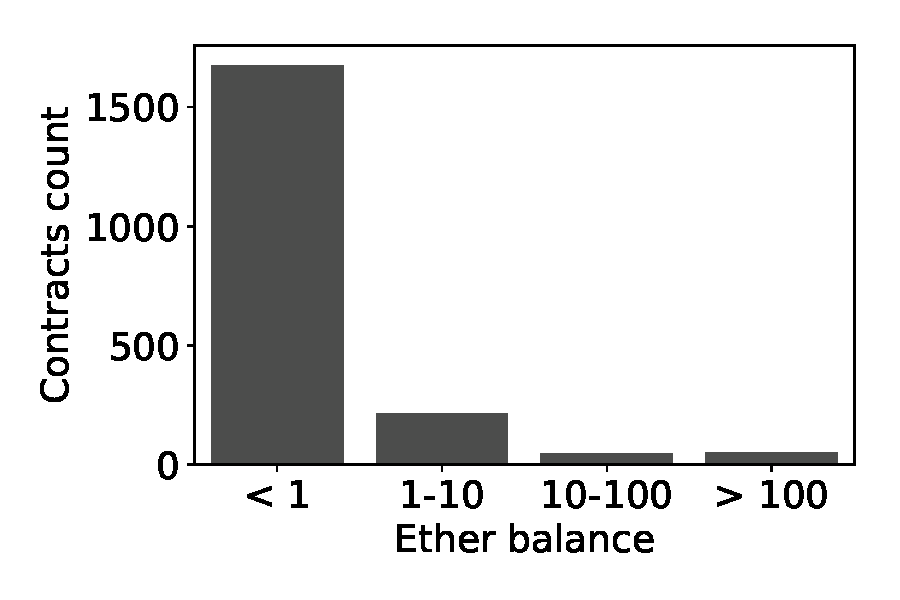
\includegraphics[width=\textwidth]{./5a-smart-contract-security/figures/balance-histogram.pdf}
    \caption{\scriptsize Ether held by contracts in our dataset\\with non-zero balance.}
    \label{fig:eth-held}
  \end{subfigure}
  \begin{subfigure}{.49\columnwidth}
    \centering
    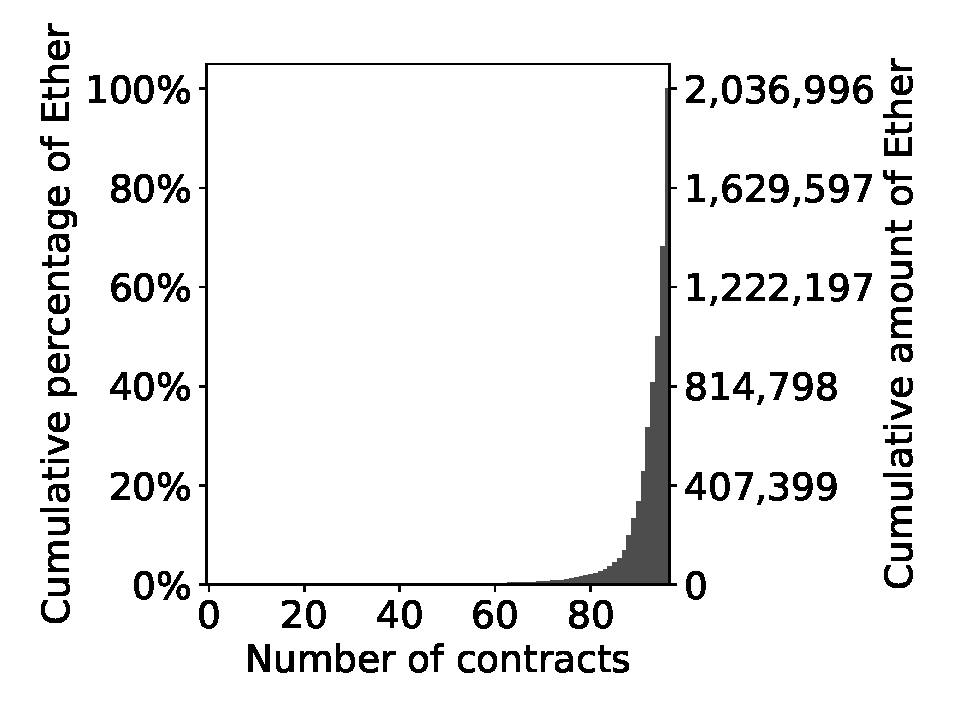
\includegraphics[width=\textwidth]{./5a-smart-contract-security/figures/cumulative-ether.pdf}
    \caption{\scriptsize Cumulative Ether held in the 96\\contracts in our dataset containing at least 10 ETH.}
    \label{fig:cumulative-eth}
  \end{subfigure}
  \caption{Ether held in contracts: describing the distribution.}
\end{figure}

\subsection{Discussion}
\label{sec:5a:discussion}

Even considering the limitations of our system, it is clear that the exploitation of smart contracts is vastly lower than what could be expected. In this section, we present some of the factors we think might be impacting the actual exploitation of smart contracts.

% \subsection{Contracts holding money}

We believe that a major reason for the difference between the number of vulnerable contracts reported and the number of contracts exploited is the distribution of Ether among contracts. Indeed, only about~\empirical{2,000} out of the~\VulnerableContracts contracts in our dataset contain Ether, and most of these contracts have a balance lower than~\empirical{1} ETH.
We show the balance distribution of the contracts containing Ether in our dataset in \autoref{fig:eth-held}. Furthermore, the \empirical{top 10 contracts} hold about~\empirical{95\%} of the total Ether. We show the cumulative distribution of Ether within the contracts containing more than~\empirical{10 ETH} in \autoref{fig:cumulative-eth}. This shows that, as long as the top contracts cannot be exploited, the total amount of Ether that is actually at stake will be nowhere close to the upper bound of ``vulnerable'' Ether.

To make sure this fact generalizes to the whole Ethereum blockchain and not only our dataset, we also fetch the balances for all existing contracts. This gives a total of~\empirical{15,459,193} contracts. Out of these, we find that only~\empirical{463,538} contracts have a non-zero balance, which is merely 3\% of all the contracts. Out of the contracts with a non-zero balance, the top 10 contracts account for \empirical{54\%} of the total amount of Ether, the top 100 for \empirical{92\%} and the top 1000 for \empirical{99\%}. This shows that our dataset follows the same trend as the Ethereum blockchain in general: a very small amount of contracts hold most of the wealth.

\point{Manual inspection of high-value contracts}
We decide to manually inspect the top~\empirical{6} contracts~ ---~i.e contracts with the highest balances at the time of writing~ ---~marked as vulnerable by any of the tools in our dataset. We focused on the top~\empirical{6} because it happened to be the number of contracts which currently hold more than~\empirical{100,000 ETH}. These contracts hold a total of~\empirical{1,695,240} ETH, or~\empirical{83\%} of the total of \empirical{2,037,521 ETH} currently held by all the contracts in our dataset.

\begin{table}[tb]
  \centering
  \caption{Top \empirical{six} most valuable contracts flagged as vulnerable by at least one tool.}
  \label{fig:vulnerable-active}
  \small
  \setlength{\tabcolsep}{1.5pt}
  \begin{tabular}{lrll}
    \toprule
    \bf Address                                                      & \bf ETH balance & \bf Deployed & \bf Flagged Vulnerabilities \\
    \midrule
    \addr[\footnotesize]{0xde0b295669a9fd93d5f28d9ec85e40f4cb697bae} & 649,493         & 2015-08-08   & Oyente: \vre                \\
    \midrule
    \addr[\footnotesize]{0x7da82c7ab4771ff031b66538d2fb9b0b047f6cf9} & 369,023         & 2016-11-10   & MadMax:~\vle, Zeus:~\vio    \\
    \midrule
    \addr[\footnotesize]{0x851b7f3ab81bd8df354f0d7640efcd7288553419} & 189,232         & 2017-04-18   & MadMax:~\vle                \\
    \midrule
    \addr[\footnotesize]{0x07ee55aa48bb72dcc6e9d78256648910de513eca} & 182,524         & 2016-08-08   & Securify:~\vre              \\
    \midrule
    \addr[\footnotesize]{0xcafe1a77e84698c83ca8931f54a755176ef75f2c} & 180,300         & 2017-06-04   & MadMax:~\vle                \\
    \midrule
    \addr[\footnotesize]{0xbf4ed7b27f1d666546e30d74d50d173d20bca754} & 124,668         & 2016-07-16   & Securify:~\vto,~\vue;       \\
                                                                     &                 &              & Zeus:~\vle,~\vio            \\
    \bottomrule
  \end{tabular}
\end{table}

\begin{investigation}{0xde0b295669a9fd93d5f28d9ec85e40f4cb697bae}
  The source code for this contract is not available on Etherscan. However, we discovered that this is the multi-signature wallet of the Ethereum foundation~\cite{ether-foundation-contract-reddit} and that its source code is available on GitHub~\cite{ether-foundation-contract-code}. We inspect the code and find that the only calls taking place require the sender of the message to be an owner. This by itself is enough to prevent any re-entrant call, as the malicious contract would have to be an owner, which does not make sense. Furthermore, although the version of Oyente used in the paper reported the reentrancy, more recent versions of the tool did not report this vulnerability anymore. Therefore, we safely conclude that the reentrancy issue was a false alert.
\end{investigation}

We were able to inspect~\empirical{4} of the~\empirical{5} remaining contracts.
The contract at address\\\addr{0x07ee55aa48bb72dcc6e9d78256648910de513eca} is the only one for which we were unable to find any information. The second, third and fifth contracts in the list were also multi-signature wallets and exploitation would require a majority owner to be malicious. For example, for Ether to get locked, the owners would have to agree on adding enough extra owners so that all the loops over the owners result in an out-of-gas exception. The contract at address~\addr{0xbf4ed7b27f1d666546e30d74d50d173d20bca754} is a contract known as \lstinline{WithDrawDAO}~\cite{withdraw-dao}. We did not find any particular issue, but it does use a delegate pattern which explains the locked Ether vulnerability marked by Zeus.

Overall, all the contracts from \autoref{fig:vulnerable-active} that we could analyze seemed quite secure and the vulnerabilities flagged were not exploitable.
Although there are some very rare cases that we present in \autoref{sec:5a:related} where contracts with high Ether balances are being stolen, these remain exceptions. The facts we presented up to now help us confirm that the amount of Ether at risk on the Ethereum blockchain is nowhere as close as what is claimed~\cite{DBLP:conf/ndss/KalraGDS18,Grech2018}.
We now present a thorough investigation of the high-value contracts.

\begin{investigation}{0xde0b295669a9fd93d5f28d9ec85e40f4cb697bae}
  This contract has been flagged as being vulnerable to reentrancy by Oyente. For a contract to be a victim of a reentrancy attack, it must \lstinline{CALL} another contract, sending it enough gas to be able to perform the re-entrant call. In Solidity terms, this means that the contract has to invoke \lstinline{address.call} and not explicitly set the gas limit. By looking at the source code~\cite{ether-foundation-contract-code}, we find 2 such instances: one at line 352 in the \lstinline{execute} function and another at line 369 in the \lstinline{confirm function}. The \lstinline{execute} is protected by the \lstinline{onlyowner} modifier, which requires the caller to be an owner of the wallet. This means that for a re-entrant call to work, the malicious contract would need to be one of the owners of the wallet in order to work. The \lstinline{confirm} function is protected by the \lstinline{onlymanyowners} modifier, which requires at least n owners to agree on confirming a particular transaction before it is executed, where n is agreed upon at contract creation time. Furthermore, \lstinline{confirm} will only invoke \lstinline{address.call} on a transaction previously created in the \lstinline{execute} function.
\end{investigation}

\begin{investigation}{0x7da82c7ab4771ff031b66538d2fb9b0b047f6cf9}
  This is the contract for the multi-signature wallet of the Golem project~\cite{golem-project} and uses a well-known multi-signature implementation. We use the source code available on Etherscan to perform the audit.
  This contract is marked with two vulnerabilities, locked Ether by MadMax and integer overflow by Zeus.

  We first focus on the locked Ether which is due to an unbounded mass operation~\cite{Grech2018}.
  An unbounded mass operation is flagged when a loop is bounded by a variable whose value could increase, for example, the length of an array.
  This is because if the number of iterations becomes too large the contract would run out of gas every time, which could indeed result in locked funds.
  All the loops except two of them are bound by the total number of owners. As owners can only be added if enough existing owners agree, running out of gas when looping on the number of owners cannot happen unless the owners agree.
  The two other loops are part of the \lstinline{filterTransactions} that loops over the total number of transactions.
  However, this function is only used by two external getters, \lstinline{getPendingTransactions} and \lstinline{getExecutedTransactions} and could therefore not result in the Ether getting locked.
  In the worst case, these getters could become unusable, which would not be a security issue.
  Nevertheless, this is indeed an issue that should be fixed, most likely by limiting the maximum number of transactions that can be retrieved by \lstinline{getPendingTransactions} and \lstinline{getExecutedTransactions}.

  Next, we look for possible integer overflows. All loops discussed above use an \lstinline{uint} as a loop index. In Solidity, \lstinline{uint} is a \lstinline{uint256} which makes it impossible to overflow here, given that neither the number of owners nor transactions could ever reach such a number. The only other arithmetic operation performed is \lstinline{owners.length - 1} in the function \lstinline{removeOwner} at line 103. This function checks that the owner exists, which means that \lstinline{owners.length} will always be at least 1 and \lstinline{owners.length} can therefore never underflow.
\end{investigation}

\begin{investigation}{0x851b7f3ab81bd8df354f0d7640efcd7288553419}
  This contract is also a multi-sig wallet, this time owned by Gnosis Ltd.\footnote{\url{https://gnosis.io/}}
  We use the source code available on Etherscan to perform the audit.
  The contract looks very similar to the one used by \addr{0x7da82c7ab4771ff031b66538d2fb9b0b047f6cf9} and has also been marked by MadMax as being vulnerable to locked Ether because of unbounded mass operations.
  Again, we look at all the loops in the contract and find that as in the previous contract, it loops exclusively on owners and transactions. As in the previous contract, we assume looping on the owners is safe and look at the loops over the transactions. This contract has two functions looping over transactions, \lstinline{getTransactionCount} at line 303 and \lstinline{getTransactionIds} at line 351. Both functions are getters which are never called from within the contract. Therefore, no Ether could ever be locked because of this. Unlike the previous contract, \lstinline{getTransactionIds} allows to set the range of transactions to return, therefore making the function safe to unbounded mass operations. However, \lstinline{getTransactionCount} does loop over all the transactions, and as before, could therefore become unusable at some point, although it is highly unlikely.
\end{investigation}

\begin{investigation}{0xcafe1a77e84698c83ca8931f54a755176ef75f2c}
  This contract is again a multi-sig wallet, this time owned by the Aragon project\footnote{\url{https://aragon.org/}}. We also use the contract published on Etherscan for the audit. It appears that the source code for this contract is exactly the same as the one of \addr{0x851b7f3ab81bd8df354f0d7640efcd7288553419} except that it is missing a contract called \lstinline{MultiSigWalletWithDailyLimit}. This contract was also flagged as being at risk of unbounded mass operations by MadMax, the conclusions are therefore exactly the same as for the previous contract.
\end{investigation}

\begin{investigation}{0xbf4ed7b27f1d666546e30d74d50d173d20bca754}
  This contract is the only one which is very different from the previous ones. It is the \lstinline{WithdrawDAO} contract, which has been created for users to get their funds back after TheDAO incident~\cite{securities2017}. We use the source code from Etherscan to audit the contract.
  This contract has been flagged with several vulnerabilities: Securify flagged it with transaction order dependency and unhandled exception, while Zeus flagged it with locked ether and integer overflow.
  The contract has two very short functions: \lstinline{withdraw} which allows users to convert their TheDAO tokens back to Ether, and the \lstinline{trusteeWithdraw} which allows sending funds which cannot be withdrawn by regular users to a trusted address.
  We first look at the transaction order dependency. As any user will only ever be able to receive the total amount of tokens he possesses, the order of the transaction should not be an issue in this contract. We then look at unhandled exceptions. There is indeed a call to \lstinline{send} in the \lstinline{trusteeWithdraw} which is not checked. Although it is not particularly an issue here, as this does not modify any other state, an error should probably be thrown if the call fails. We then look at locked ether. The contract is flagged with locked ether because of what Zeus classifies as a ``failed send''. This issue was flagged because if the call to \lstinline{mainDAO.transferFrom} would always revert, then the call to \lstinline{msg.sender.send} would never be reached, indeed preventing from reclaiming funds.
  However, in this context, \lstinline{mainDAO} is a trusted contract and it is, therefore, safe to assume that \lstinline{mainDAO.transferFrom} will not always fail. Finally, we look at the integer overflow issue. The only place where an overflow could occur is in \lstinline{trusteeWithdraw} at line 23. This could indeed overflow without some assumptions on the different values. For this particular contract, the following assumptions are made.

  \lstset{
    basicstyle=\ttfamily,
    mathescape
  }
  \begin{align*}
     & \text{\lstinline{this.balance}} \mbox{\footnotesize $+$} \text{\lstinline{mainDAO.balanceOf(this)}} \mbox{\footnotesize $\geq$} \text{\lstinline{mainDAO.totalSupply()}} \\
     & \text{\lstinline{mainDAO.totalSupply()}} \mbox{\footnotesize $>$} \text{\lstinline{mainDAO.balanceOf(this)}}
  \end{align*}

  As long as these assumptions hold, which was the case when the contract was deployed, this expression will never overflow. Indeed, if we note $t$ the time before the first call to \lstinline{trusteeWithdraw} and $t + 1$ the time after the first call, we will have
  \begin{lstlisting}
this.balance$_{t+1}$ = this.balance$_t$ - (
  this.balance$_t$ + mainDAO.balanceOf(this)
                - mainDAO.totalSupply())
 = -mainDAO.balanceOf(this)+mainDAO.totalSupply()
\end{lstlisting}

  % \begin{align*}
  %   \text{\lstinline{this.balance}}_{t+1} &\mbox{\footnotesize $=$} \text{\lstinline{this.balance}}_t \mbox{\footnotesize $-$}\\
  %   (\text{\lstinline{this.balance}}_t &\mbox{\footnotesize $+$}\text{\lstinline{mainDAO.balanceOf(this)}} \mbox{\footnotesize $-$} \text{\lstinline{mainDAO.totalSupply()}})\\
  %   &\mbox{\footnotesize $=$} \mbox{\footnotesize $-$}\text{\lstinline{mainDAO.balanceOf(this)}} \mbox{\footnotesize $+$}\text{\lstinline{mainDAO.totalSupply()}}
  % \end{align*}

  which means that every subsequent call will compute the following.

  \begin{lstlisting}
this.balance$_{t+1}$ + mainDAO.balanceOf(this) -
                       mainDAO.totalSupply()
 = -mainDAO.balanceOf(this)+mainDAO.totalSupply()+
   mainDAO.balanceOf(this) - mainDAO.totalSupply()
 = 0
\end{lstlisting}

  % \begin{align*}
  %   &\text{\footnotesize\lstinline{this.balance}}_{t+1} + \text{\footnotesize\lstinline{mainDAO.balanceOf(this)}} - \text{\footnotesize\lstinline{mainDAO.totalSupply()}}\\
  %   &= -\text{\footnotesize\lstinline{mainDAO.balanceOf(this)}} +\text{\footnotesize\lstinline{mainDAO.totalSupply()}} + \\
  %   &\quad\text{\footnotesize\lstinline{mainDAO.balanceOf(this)}} - \text{\footnotesize\lstinline{mainDAO.totalSupply()}}\\
  %   &= 0
  % \end{align*}

  This will always result in sending $0$ and will therefore not cause any overflow. If some money is newly received by the contract, the amount received will be transferred the next time \lstinline{trusteeWithdraw} is called.
\end{investigation}


% \subsection{Lifespan of contracts}
% As described in \autoref{sec:5a:background}, due to smart contracts deployed on Ethereum being immutable, any update to a contract requires the deployment of a new one. As a result, smart contracts have a relatively short lifespan. We define the lifespan of a smart contract as the number of days elapsed between the first and the last transaction sent to it.

% \begin{figure}[tb]
%     % \includegraphics[width=\columnwidth]{./figures/recency.pdf}
%     \caption{Capturing the recency of active contract use.}
%     \label{fig:recency}
% \end{figure}
% \autoref{fig:recency}...


\subsection{Related Work}
\label{sec:5a:related}

% Some major smart contracts exploits have been observed on Ethereum in recent years~\cite{securities2017}.
% These attacks have been analyzed and classified~\cite{atzei2017} and many tools and techniques have emerged to prevent such attacks~\cite{harz2018towards,Dika2017}.
% Recent literature has also shown how attacks on Ethereum are evolving with time~\cite{255252}.
% In this section, we will first provide details about two of the most prominent historic exploits and then present existing work aimed at increasing smart contract security.

% \subsubsection{Motivating Large-scale Exploits}
% \point{TheDAO exploit}
% TheDAO exploit~\cite{securities2017} is one of the most infamous bugs on the Ethereum blockchain. Attackers exploited a reentrancy vulnerability~\cite{atzei2017} of the contract which allowed for the draining of the contract's funds. The attacker contract could call the function to withdraw funds in a re-entrant manner before its balance on TheDAO was reduced, making it indeed possible to freely drain funds. A total of more than 3.5 million Ether were drained. Given the severity of the attack, the Ethereum community finally agreed on hard forking.
% %
% \point{Parity wallet bug}
% The Parity Wallet bug~\cite{Breidenbach} is another prominent vulnerability on the Ethereum blockchain which caused 280 million USD worth of Ethereum to be frozen on the Parity wallet account. It was due to a very simple vulnerability: a library contract used by the parity wallet was not initialized correctly and could be destructed by anyone. Once the library was destructed, any call to the Parity wallet would then fail, effectively locking all funds.

%\subsection{Other contract vulnerabilities}
%Recent research have proposed different taxonomies of smart contract vulnerabilities~\cite{luu2016a,atzei2017,Nikolic2018a}. Here, we will present a few classes of bugs that enter most of the proposed taxonomies.

% \subsection{Analysis Tools For Finding Vulnerabilities}

% \subsubsection{Analyzing and Verifying Smart Contracts}
% \label{ssec:related-analysis-tools}
\subsubsection{Previous work}
There have been a lot of efforts in order to prevent exploits and to make smart contracts more secure in general.
We will here present some of the tools and techniques which have been presented in the literature and, when relevant, describe how they compare to our work.

Analysis tools can roughly be divided into two categories: static analysis and dynamic analysis tools.
Using the term ``static'' quite loosely, static analysis tools can be defined as tools which catch bugs or vulnerabilities without the need to deploy the smart contracts.
Runtime analysis tools try to detect these by executing the deployed contracts.
Our tool fits into the second category.

\point{Static analysis tools} Static analysis tools have been the main focus of research.
This is understandable, given how critical it is to avoid vulnerabilities in a deployed contract.
Most of these tools work by analysing either the bytecode or the high-level code of the contract and checking for known vulnerable patterns in these.

Oyente~\cite{luu2016a} is one of the first tools which has been developed to analyze smart contracts.
It uses symbolic execution in combination with the Z3 SMT solver~\cite{de2008z3} to check for the following vulnerabilities: transaction ordering dependency, reentrancy and unhandled exceptions.

ZEUS~\cite{DBLP:conf/ndss/KalraGDS18} is a static analysis tool which works on the Solidity smart contract and not on the bytecode, making it appropriate to assist development efforts rather than to analyze deployed contracts, for which Solidity code is typically not available.
Zeus transpiles XACML-styled~\cite{XACML} policies to be enforced and the Solidity contract code into LLVM bitcode~\cite{lattner2004llvm} and uses constrained Horn clauses~\cite{bjorner2012program,mcmillan2007interpolants} over it to check that the policy is respected.

Securify~\cite{Tsankov2018} is a static analysis tool which checks the security properties of the EVM bytecode of smart contracts.
The security properties are encoded as patterns written in a Datalog-like~\cite{ullman1984principles} domain-specific language and checked either for compliance or violation.
Securify infers semantic facts from the contract and interprets the security patterns to check for their violation or compliance by querying the inferred facts.
This approach has many similarities with ours, using Datalog to express vulnerability patterns.
The major difference is that Securify works on the bytecode directly while our tool works on the execution traces.

MadMax~\cite{Grech2018} has similarities with Securify, as it also encodes properties of the smart contract into Datalog, but it focuses on vulnerabilities related to gas.
It is the first tool to detect ``unbounded mass operations'', where a loop is bounded by a dynamic property such as the number of users, causing the contract to always run out of gas passed a certain number of users.
MadMax is built on top of the decompiler implemented by Vandal~\cite{Brent2018} and is performant enough to analyze all the contracts of the Ethereum blockchain in only 10 hours.

Several other static analysis tools have been developed, some, such as SmartCheck~\cite{Tikhomirov2017}, being quite generic and handling many classes of vulnerabilities, and others being more domain-specific, such as Osiris~\cite{torres2018osiris} focusing on integer overflows, Maian~\cite{Nikolic2018a} focusing on unrestricted actions or Gasper~\cite{Chen2017} focusing on costly gas patterns.
More recently, ETHBMC~\cite{251546} was designed to also support inter-contract relations, cryptographic hash functions and memcopy-style operations.

Finally, there have also been some efforts to formally verify smart contracts.
\cite{Hirai2017} is one of the first efforts in this direction and defines the EVM using Lem~\cite{mulligan2014lem}, which allows generating definitions for theorem provers such as Coq~\cite{barras1997coq}.
\cite{Grishchenko2018} presents a complete small-step semantics of EVM bytecode and formalizes it using the F* proof assistant~\cite{SwamyCFSBY11}.
A similar effort is made in~\cite{Hildenbrandt2018} to give an executable formal specification of the EVM using the K Framework~\cite{rosu-serbanuta-2010-jlap}.
VerX~\cite{permenev2019verx} is also a recent work allowing users to write properties about smart contracts which will be formally verified by the tool.

\point{Dynamic analysis tools} Although dynamic analysis tools have been less studied than their static counterpart, some work has emerged in recent years.

One of the first works in this line is ContractFuzzer~\cite{Jiang2018}.
As its name indicates, it uses fuzzing to find vulnerabilities in smart contracts and is capable of detecting a wide range of vulnerabilities such as reentrancy, locked Ether or unhandled exceptions.
The tool generates inputs to the contract and checks using an instrumented EVM whether some vulnerabilities have been triggered.
An important limitation of this fuzzing approach is that it requires the Application Binary Interface of the contract, which is typically not available for contracts deployed on the main Ethereum network.

Sereum~\cite{Rodler2019} focuses on detecting reentrancy exploitation at runtime by integrating checks in a modified Go Ethereum client.
The tool analyzes runtime traces and uses taint analysis to ensure that no variable accessing the contract storage is used in a re-entrant call.
Although there are some similarities with our tool, which also analyzes traces at runtime, Sereum focuses on reentrancy while our tool is more generic, notably because vulnerabilities pattern can easily be expressed using Datalog, and allows to analyse several more classes of vulnerabilities.

teEther~\cite{Krupp2018} also works at runtime but is different from the previous works presented, as it does not try to protect contracts but rather to actively find an exploit for them. It first analyses the contract bytecode to look for critical execution paths.
Critical paths are execution paths which may result in lost funds, for example by sending money to an arbitrary address or being destructed by anyone.
To find these paths, it uses an approach close to Oyente~\cite{luu2016a}, first using symbolic execution and then the Z3 SMT solver~\cite{de2008z3} to solve path constraints.

\point{Summary} Static analysis tools are typically designed to detect \emph{vulnerable} contracts, while dynamic analysis tools are designed to detect \emph{exploitable} contracts. The only exception is Sereum, which detects contracts \emph{exploited} using reentrancy.
Our work is, to the best of our knowledge, the first attempt to detect contracts \emph{exploited} using a wide range of vulnerabilities.
This is mostly orthogonal with other works and can support analysis tool development efforts by helping to understand what type of exploitation is happening in the wild.

\subsubsection{Follow-up work}
More related work has been published since the submission of the paper this part of the chapter is based on.
We present some of these here.

TXSPECTOR~\cite{255340}, which was published soon after the first version of this section, uses a very similar approach to ours to detect reentrancy, unchecked call and suicidal contracts.
They also leverage a Datalog approach to detect vulnerabilities but first transform the transaction traces into a flow graph rather than adding facts about traces directly to the Datalog database.
While this does add expressiveness, it makes the analysis significantly more complex, resulting in some analysis timing out on some transactions.
Therefore, we believe that their approach could be complementary to ours and used to eliminate potential false positives of our approach.

\section{Conclusion}
\label{sec:conclusion}

In this paper, we surveyed the~\VulnerableContracts vulnerable contracts reported by~\PapersAnalyzed recent academic projects. We proposed a Datalog-based formulation for performing analysis over EVM execution traces and used it to analyze a total of more than~\empirical{20 million} transactions executed by these contracts. We found that at most~\NumExploitedContracts out of~\VulnerableContracts contracts have been subject to exploits but that at most~\ExploitedEther ETH (\ExploitedEtherUSD USD), or only~\PercentExploitedEther of the \EtherClaimedVulnerable ETH (\EtherClaimedVulnerableUSD USD) potentially at risk, was exploited.
Finally, we found that a majority of Ether is held by only a small number of contracts and that the vulnerabilities reported on these are either false positives or not exploitable in practice, thus providing a reasonable explanation for our results.

% Our results suggest that the impact of vulnerable smart contracts on the Ethereum blockchain had been exaggerated. We hypothesize that the main reasons for the significant gap between vulnerable and exploited are: many contracts flagged vulnerable are not in practice exploitable and most of the high-value contracts, which would be the most interesting to the attackers, fall into this category.



\section{Application Security}

One of the major defences against economic attacks in DeFi protocols is over-collateralization.
Nonetheless, factors such as price volatility may undermine this mechanism.
In order to protect protocols from suffering losses, under-collateralized positions can be \textit{liquidated}.
In this section, we present the first in-depth empirical analysis of liquidations on protocols for loanable funds (PLFs).
We examine Compound, one of the most widely used PLFs, for a period starting from its conception to September 2020.
We analyze participants' behaviour and risk appetite, in particular, to elucidate recent developments in the dynamics of the protocol.
Furthermore, we assess how this has changed with a modification in Compound's incentive structure and show that variations of only~3\% in an asset's dollar price can result in over 10m USD becoming liquidatable.
To further understand the implications of this, we investigate the efficiency of liquidators.
We find that liquidators' efficiency has improved significantly over time, with currently over~70\% of liquidatable positions being immediately liquidated.
Lastly, we provide a discussion on how a false sense of security fostered by a misconception of the stability of non-custodial stablecoins, increases the overall liquidation risk faced by Compound participants.


\subsection{Introduction}
\label{sec:5b:introduction}

As explained earlier in this chapter, Decentralized Finance (DeFi) refers to a peer-to-peer, permissionless blockchain-based ecosystem that utilizes the integrity of smart contracts for the advancement and disintermediation of traditional financial primitives. 
One of the most prominent DeFi applications on the Ethereum blockchain~\cite{wood2014ethereum} is protocols for loanable funds (PLFs)~\cite{10.1145/3419614.3423254}.
On PLFs, markets for loanable funds are established via smart contracts that facilitate borrowing and lending \cite{10.1145/3570639}.
In the absence of strong identities on Ethereum, creditor protection tends to be ensured through over-collateralization, whereby a borrower must provide collateral worth more than the value of the borrowed amount.
In the case where the value of the collateral-to-borrow ratio drops below some liquidation threshold, a borrower defaults on his position and the supplied collateral is sold off at a discount to cover the debt in a process referred to as \textit{liquidation}.
However, little is known about the behaviour of agents towards liquidation risk on a PLF.
Furthermore, despite liquidators playing a critical role in the DeFi ecosystem, the efficiency with which they liquidate positions has not yet been thoroughly analyzed.

In this section, we first lay out a framework for quantifying the state of a generic PLF and its markets over time. 
We subsequently instantiate this framework to all markets on Compound~\cite{leshner2018}, one of the largest PLFs in terms of locked funds.
We analyze how liquidation risk has changed over time, specifically after the launch of Compound's governance token.
Furthermore, we seek to quantify this liquidation risk through a price sensitivity analysis.
In a discussion, we elaborate on how the interdependence of different DeFi protocols can result in agent behaviour undermining the assumptions of the protocols' incentive structures.

\point{Contributions} This section makes the following contributions:
\begin{itemize}
    \item We present an abstract framework to reason about the state of PLFs.
    
    \item We provide an open-source implementation\footnote{\url{https://github.com/backdfund/analyzer}} of the proposed framework for Compound, one of the largest PLFs in terms of total locked funds.
    
    \item We perform an empirical analysis on the historical data for Compound, from \StartDate to \EndDate and make the following observations:
    \begin{enumerate}%[label={(\roman*)}]
    \item despite increases in the number of suppliers and borrowers, the total funds locked are mostly accounted for by a small subset of participants; 
    \item the introduction of Compound's governance token had protocol-wide implications as liquidation risk increased as a consequence of the higher risk-seeking behaviour of participants;
    \item liquidators became significantly more efficient over time, liquidating over 70\% of liquidatable positions instantly.
    \end{enumerate}
    
    \item Using our findings, we demonstrate how interactions between protocols' incentive structures can directly result in unexpected risks to participants.
\end{itemize}


% \section{Background}
\label{sec:background}
In this section we introduce preliminary concepts about blockchains and smart contracts necessary to the understanding of the rest of the paper.

\subsection{Blockchain}

% \point{Blockchain}
A blockchain, such as Bitcoin~\cite{Nakamoto} or Ethereum~\cite{wood2014ethereum}, is in essence a decentralized append-only database.
Data is added to the blockchain in the form of transactions that are grouped in blocks.
Some rules are enforced by the protocols on both transactions and blocks to ensure its correct working.
Blockchains need to be able to maintain consensus of which blocks are included.
Both Bitcoin and Ethereum use the Proof-of-Work consensus that requires block producers, often called \emph{miners}, to solve a computationally expensive puzzle to produce a new block \cite{Perez2020c}.
An important point to note is that miners are allowed to choose which transactions to include in a block and in which order to include them.
This can potentially allow miners to profit from having a transaction included before another one.
This is commonly referred to as \emph{miner-extractable value}~\cite{daian2020flash}.

\subsection{Smart Contracts}
\point{Ethereum smart contracts}
On Ethereum, smart contracts are programs written in a Turing-complete language, typically Solidity~\cite{docs:solidity}, that define a set of rules that may be invoked by any network participant. 
These programs rely on the Ethereum Virtual Machine (EVM), a low-level stack machine which executes the compiled EVM bytecode of a smart contract~\cite{wood2014ethereum}.
Each instruction has a fee measured in so-called \textit{gas}, and the total gas cost of a transaction is a fixed base fee plus the sum of all instructions' gas~\cite{albert2020gasol,Perez2020f}.
The sender of a transaction must then set a gas price, the amount of \coin{ETH} he is willing to pay per unit of gas consumed for executing the transaction.
The transaction fee is thus given by the gas price multiplied with the gas cost~\cite{werner2020step,pierro2019influence}.
Within a transaction, smart contracts can store data in logs, which are metadata specially indexed as part of the transaction.
This metadata, commonly referred to as \textit{events}, is typically used to allow users to monitor the activity of a contract externally.

\point{Oracles}
One of the major challenges smart contracts face concerns access to off-chain information, i.e. data that does not natively exist on-chain.
Oracles are data feeds into smart contracts and provide a mechanism for accessing off-chain information through some third party.
In DeFi, oracles are commonly used for price feed data to determine the real-time price of assets.
For instance, via the Compound Open Price Feed~\cite{web:compoundfinance_prices}, vetted third party reporters sign off on price data using a known public key, where the resulting feed can be relied upon by smart contracts.

\point{Stablecoins}
An alternative to volatile cryptoassets is given by stablecoins, which are priced against a peg and can be either custodial or non-custodial.
For custodial stablecoins (e.g. \coin{USDC}~\cite{web:usdc}), tokens represent a claim of some off-chain reserve asset, such as fiat currency, which has been entrusted to a custodian.
Non-custodial stablecoins (e.g. \coin{DAI}~\cite{whitepaper:maker}) seek to establish price stability via economic mechanisms specified by smart contracts.
For a thorough discussion on stablecoin design, we direct the reader to \cite{Klages-Mundt2020}.


\section{Protocols for Loanable Funds (PLF)}
\label{sec:plfs}
In this section, we introduce several concepts of Protocols for Loanable Funds (PLFs) necessary for understanding how liquidations function in DeFi on Ethereum.

\subsection{Supplying and borrowing in DeFi}
In DeFi, asset supplying and borrowing is achieved via so-called \textit{protocols for loanable funds} (PLFs)~\cite{gudgeon2020defi}, where smart contracts act as trustless intermediaries of loanable funds between suppliers and borrowers in markets of different assets.
Unlike traditional peer-to-peer lending, deposits are pooled and instantly available to borrowers.
On a DeFi protocol, the aggregate of tokens that the PLF smart contracts hold, which equals the difference between supplied funds and borrowed funds, is termed \text{locked funds}~\cite{DeFiPulse2020}.

\subsection{Interest model}
Borrowers are charged interest on the debt at a floating rate determined by a market's underlying interest rate model.
A small fraction of the paid interest is allocated to a pool of reserves, which is set aside in case of market illiquidity, while the remainder is paid out to suppliers of loanable funds.
Interest in a given market is generally accrued through market-specific, interest-bearing derivative tokens that appreciate against the underlying asset over time.
Hence, a supplier of funds receives derivative tokens in exchange for supplied liquidity, representing his share in the total value of the liquidity pool for the underlying asset.
The most prominent PLFs are Compound~\cite{web:compoundfinance} and Aave~\cite{web:aave}, with 2.5bn USD and 2.7bn USD in total funds locked respectively, at the time of writing~\cite{DeFiPulse2020}.

\subsection{Collateralization}
Given the pseudonymity of agents in Ethereum, borrow positions need to be overcollateralized to reduce the default risk.
Thereby, the borrower of an asset is required to supply collateral, where the total value of the supplied collateral exceeds the total value of the borrowed asset.
Each asset is associated with a collateralization ratio, namely the minimum collateral-to-borrow ratio when the asset is used to collateralize a new borrow position.
For example, in order to borrow 100 USD worth of \coin{DAI} with \coin{ETH} as collateral at a collateralization ratio of 125\%, a borrower would have to lock 125 USD worth of \coin{ETH} to collateralize the borrow position.
Thus, the protocol limits monetary risk from defaulted borrow positions, as the underlying collateral of a defaulted position can be sold off to recover the debt.
The inverse of the collateralization ratio is referred to as the \textit{collateral factor}, which is the amount of a deposit that may be used as collateral.
For example, if the collateralization ratio on a PLF for the market of \coin{DAI} is $125$\%, the collateral factor would be $0.8$, implying that for each \$$1$ deposit of \coin{DAI}, the supplier may borrow \$$0.8$ worth of some other asset.

\subsection{Liquidation}
The process of selling a borrower's collateral to recover the debt value upon default is referred to as \textit{liquidation}.
A borrow position can be liquidated once the value of the collateral falls below some pre-determined liquidation threshold, i.e. the minimum acceptable collateral-to-borrow ratio.
Any network participant may liquidate these positions by paying the debt asset to acquire the underlying collateral at a discount.
Hence, liquidators are incentivised to actively monitor others' collateral-to-borrow ratios. 
Note that in practice, the amount of liquidable collateral that a single liquidator can purchase may be capped.  

\subsection{Leveraging}
In finance, leverage refers to borrowed funds being used as the funding source for additional, typically more risky capital.
In DeFi, leverage is the fundamental component of PLFs, as a borrower is required to first take up the role of a supplier and deposit funds which are to be used as leverage for his borrow positions, as we have just seen.
The typical aim of leveraging is to generate higher returns through increased exposure to a particular investment.
For example, a borrower wanting to gain increased exposure to \coin{ETH} may:
\begin{enumerate}
\item Supply \coin{ETH} on a PLF.
\item Leverage the deposited \coin{ETH} to borrow \coin{DAI}.
\item Sell the purchased \coin{DAI} for \coin{ETH}.
\item Repeat steps $1$ to $3$ as desired. 
\end{enumerate}

This behavior essentially enables users to construct so-called \textit{leveraging spirals}, whereby a user repeatedly re-supplies borrowed funds in order to get increased exposure to some crypto-asset. 
However, increased exposure comes at the cost of higher downside risk, i.e., the risk of the value of the leveraged asset or borrowed asset to decrease due to changing market conditions.

\subsection{Use Cases of PLFs}
We present the different incentives\footnote{Note that leverage on a PLF in DeFi may in part be motivated by tax benefits, as certain jurisdictions may not tax capital gains on borrowed funds. 
However, a detailed analysis of this lies outside the scope of this paper.} an agent may have for borrowing from and/or supplying to a PLF:
\begin{description}
    \item[Interest] Suppliers of funds are incentivised by interest which accrues on a per block basis.

    \item[Leveraged long position] To take on a long position of an asset refers to purchasing an asset with the expectation that it will appreciate in value. 
    These positions can be taken on a PLF by leveraging the asset on which the long position shall be taken.

    \item[Leveraged short position] A short position refers to borrowing funds of an asset, which one believes will depreciate in value. 
    Consequently, the taker of a short position sells the borrowed asset, only to repurchase it and pay back the borrower once the price has fallen, while profiting from the price change of the shorted asset.
    This can be achieved by taking on a leveraged borrow position of a stablecoin, where the locked collateral is the asset to short.

    \item[Liquidity mining] As a means to attract liquidity, PLFs may distribute governance tokens to their liquidity providers.
    The way these tokens are distributed depends on the PLF. 
    For instance, on Compound, the governance token \coin{COMP}\footnote{Contract address: \contractaddr{0xc00e94cb662c3520282e6f5717214004a7f26888}} is distributed among users across markets proportionally to the total dollar value of funds borrowed and supplied.
    This directly incentivises users to mine liquidity in a market through leveraging in order to receive a larger share of governance tokens.
    For example, a supplier of funds in market $A$ can borrow against his position additional funds of $A$, at the cost of paying the difference between the earned and paid interest. 
    The incentive for pursuing this behaviour exists if the reward (i.e.\ the governance token) exceeds the cost of borrowing.
    
    \item[Token utility] An agent may be able to obtain a token from a PLF which has some desired utility.
    For example, for the case of governance tokens, the desired token utility could be the right to participate in protocol governance or a claim on protocol earnings.
    
    
\end{description}


% \subsection{Supplying and borrowing incentives}
% \todo{maybe integrate this with the previous subsection?}
% As the total liquidity in DeFi is fragmented across protocols, a constant competition over deposits persists, commonly referred to as \textit{liquidity mining}.
% Apart from earning interest on deposited funds on PLFs, liquidity providers may also earn rewards by receiving protocol-specific tokens. This is commonly seen for not only PLFs \cite{web:compoundfinance}, but also other types of DeFi protocols such as automated market makers~\cite{web:balancer,web:curve} and yield aggregators~\cite{web:yearn}.
% While these protocol-specific tokens are typically intended for participation in protocol governance, they are also tradable on the open market and thus provide further financial incentive to liquidity providers.

% % While PLFs require borrowers to overcollateralize the debt to provide security to a protocol, a mechanism that may appear rather impractical for borrowers.
% Despite the cost of over-collateralization, borrowing can also be incentivized in various ways.
% Firstly, a user may be attracted by the utility of the borrowed token, which could be the right to participate in protocol governance in the case of governance tokens, or protocol earnings that a token holder is entitled to.
% % there may be several motivations for borrowing cryptoassets.
% Furthermore, with a protocol that rewards 
% % liquidity providers 
% suppliers and borrowers
% with some native token (e.g. a governance token), a user may chase those token rewards by supplying, borrowing and resupplying the borrowed funds back to the market, giving rise to leveraged borrowing spirals seen above.
% % whereby a borrower resupplies the borrowed funds for the sole purpose of receiving a larger share of the distributed token rewards.
% % A third incentive for borrowing could come in the form of tax avoidance by borrowing and lending instead of buying and selling cryptoassets. 


\subsection{Methodology}
\label{sec:5b:methodology}

In this section, we describe our methodology for the different analyses we perform about leveraging in PLFs.
To be able to quantify the extent of leveraged positions over time, we first introduce a state transition framework for tracking the supply and borrow positions across all markets on a given PLF.
We then describe how we instantiate this framework on the Compound protocol using on-chain events data.

\subsubsection{Definitions}

Throughout the section, we use the following definitions in the context of PLFs:

\begin{description}
\item[Market] A smart contract acting as the intermediary of loanable funds for a particular crypto asset, where users supply and borrow funds. 

\item[Supply] Funds deposited to a market that can be loaned out to other users and used as collateral against depositors' borrow positions.

\item[Borrow] Funds loaned out to users of a market.

\item[Collateral] Funds available to back a user's aggregate borrow positions.

\item[Locked funds] Funds remaining in the PLF smart contracts, equal to the difference between supplied and borrowed funds.

\item[Supplier] A user who deposits funds to a market.

\item[Borrower] A user who borrows funds from a market. Since a borrow position must be collateralized by deposited funds, a borrower must also be a supplier.

\item[Liquidator] A user who purchases a borrower's supply in a market when the borrower's collateral-to-borrow ratio falls below some threshold.
\end{description}


\subsubsection{States on a PLF}
In this section, we provide a formal definition of the state of a PLF.
We denote $\mathfrak{P}_t$ as the global state of a PLF at time $t$.
For brevity, in the following definitions, we assume that all the values are at a given time $t$.
We define the global state of the PLF as
\[
  \mathfrak{P} = (\mathcal{M},\Gamma, \mathcal{P}, \Lambda)
\]
where $\mathcal{M}$ is the set of states of individual markets, $\Gamma$ is the price the Oracle used, $\mathcal{P}$ is the set of states of individual participants and $\Lambda \in (0, 1)$ is the close factor of the protocol, which specifies the upper bound on the amount of collateral a liquidator may purchase.

We define the state of an individual market
$m \in \mathcal{M}$ as 
$$m = (\mathcal{I}, \mathcal{B}, \mathcal{S}, \mathcal{C})$$
where
$\mathcal{I}$ is the market's interest rate model,
$\mathcal{B}$ is the total borrows,
$\mathcal{S}$ is the total supply of deposits,
% $\mathcal{R}$ is the total reserves,
% $\mathcal{F}$ is the reserve factor,
and $\mathcal{C}$ is the collateral factor.
% ,
% and $\mathcal{P}_t^j$ the set of participants in market $m_t^j$.

$\mathcal{P}^m$ is the state of all participants in market $m$ and the positions of a participant $P$ in this market is defined as
\[
  P^m = (B^m,S^m)
\]
where $B^m$ and $S^m$ are respectively the total borrow positions and total supplied deposits of a market participant in market $m$.

For a given market $m$, the total deposits supplied $\mathcal{S}^m$ is thus given by:
\begin{equation}
    \mathcal{S}^m = \sum_{P^m\in \mathcal{P}^m} S^m
\end{equation}

Similarly, the market's total borrows $\mathcal{B}^m$ is given by:
\begin{equation}
    \mathcal{B}^m = \sum_{P^m\in \mathcal{P}^m} B^m
\end{equation}

The state of a participant $P$ is liquidatable if the following holds: 
% \begin{equation}
%     \frac{\sum_{m\in \mathcal{M}}
%     \Big\{\left[S^{m} \cdot \mathcal{C} + \mathcal{I}(S^m)\right] \cdot \Gamma(m)\Big\}
%     }{
%     \sum_{m\in \mathcal{M}} \Big\{\left[B^m + \mathcal{I}(B^m)\right] \cdot \Gamma(m)\Big\}}
%     < \mathcal{K}
%     \label{eq:liqcond}
% \end{equation}

\begin{equation}
    \frac{\sum_{m\in \mathcal{M}}
    \Big\{\left[S^{m} \cdot \mathcal{C} + \mathcal{I}(S^m)\right] \cdot \Gamma(m) \cdot \mathcal{K}^m \Big\}
    }{
    \sum_{m\in \mathcal{M}} \Big\{\left[B^m + \mathcal{I}(B^m)\right] \cdot \Gamma(m)\Big\}}
    < 1
    \label{eq:liqcond}
\end{equation}
where $\Gamma(m)$ returns the price of the underlying asset denominated in a predefined numéraire (e.g. USD), $\mathcal{I}(S^m)$ returns the interest earned with supply $S^m$, $\mathcal{I}(B^m)$ returns the interest accrued with borrow $B^m$, and $\mathcal{K}^m \leq 1$ denotes the liquidation threshold of market $m$. In Compound, liquidation threshold $\mathcal{K}^m$ is set to be constant at 100\% protocol-wide, whereas with other protocols such as Aave, $\mathcal{K}^m$ is specific to the collateral asset from market $m$, and can be dynamically adjusted when the risk level of the asset changes. 


The transition from a state of a market $m$ from time $t$ to $t+1$ is given by some state transition $\sigma$, such that $m_{t}\xrightarrow[]{\sigma}m_{t+1}$. 

\subsubsection{Leveraging Spirals on a PLF}
\label{ssec:leveraging-spirals-meth}
Here we examine the workings of leveraging in DeFi using a PLF. 
We assume a speculator on some volatile asset $B$, holds initial capital $\alpha$ in $B$.
In order to increase his exposure to $B$, the speculator may borrow a stable asset $A$ against his $\alpha$ on a PLF at a collateralization ratio $\delta>1$.
For simplicity, we shall assume in this illustrative example that a speculator will leverage his position on the same PLF.
Note that the cost of borrowing is given by some floating interest rate $\gamma$ for the specific asset market.
In return for his collateral, the borrower receives $\frac{\alpha}{\delta}$ in the volatile asset $B$.
As the debt is denominated in units of a stable asset (e.g. \coin{DAI}), the borrower has an upper limit on his net debt, remaining unaffected by any volatility in the value of asset $A$.
In order to leverage his position, the debt denominated in $A$ may be used to buy\footnote{In practice this may be done via automated market makers \cite{xu2021dexamm} (e.g. Uniswap~\cite{whitepaper:uniswap}) or via decentralized exchanges~\cite{web:dydx}.} additional units of asset $B$, which can subsequently be used to collateralise a new borrow position.
This process is illustrated in \autoref{fig:plf-leverage} and can be repeated numerous times, by which the total exposure to asset $A$, the underlying collateral to the total debt in asset $A$, increases at a decaying rate.

% Explain how an agent can leverage a position in DeFi: this diagram is a draft
\begin{figure}[tbp]
    \centering
    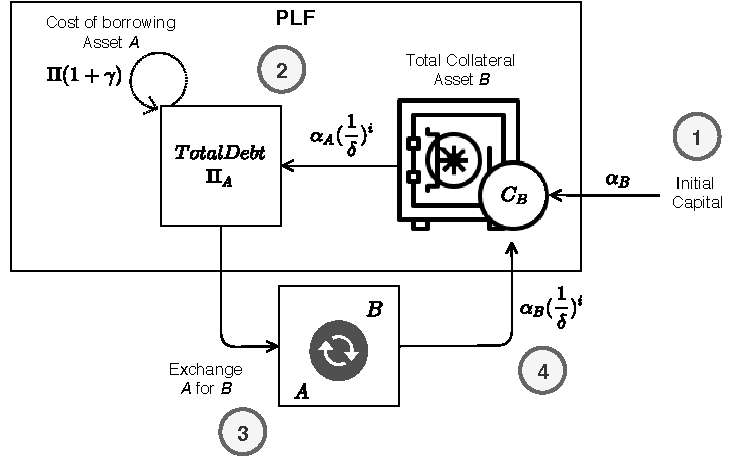
\includegraphics[width=0.8\textwidth]{5b-economic-security/figures/leveraging.pdf}
    \caption[Steps of leveraging using a PLF]{The steps of leveraging using a PLF. \textbf{1.} Initial capital $\alpha_{B}$ in asset $B$ is deposited as collateral to borrow asset $A$. \textbf{2.} Interest accrues over the debt of the borrow position for asset $B$. \textbf{3.} The borrowed asset $A$ is sold for asset $B$ on the open market. \textbf{4.} The newly purchased units of asset $B$ are locked as collateral for a new borrow position of asset $A$.}
    \label{fig:plf-leverage}
\end{figure}

The total collateral $\mathcal{C}$ a borrower must post through a borrow position with a leverage factor $k$, a collateralization ratio $\delta$ and an initial capital amount $\alpha$ can be expressed as $\sum_{i=0}^{k}\frac{\alpha}{\delta^i}$.
Hence, the total debt $\Pi$ for the corresponding borrow position is:
\begin{equation}
    \Pi = \biggl(\sum_{i=1}^{k} \frac{\alpha}{\delta^i}\biggl) \cdot (1+\gamma)
    \label{eq:debt}
\end{equation}
where $\gamma$ is the interest rate.
Note that Equation~\eqref{eq:debt} assumes a borrower uses the same collateralization ratio $\delta$ for his positions, as well as that all debt is taken out for the same asset on the same PLF and hence the floating interest rate is shared across all borrow positions. 

% \subsection{Cost of Leveraging}


% \subsection{Use Cases of Leveraging in DeFi}
% We identify three main use cases for leveraging in DeFi:

% \point{Leveraged long position} To take on a long position of an asset refers to purchasing an asset with the expectation that it will appreciate in value. 
% In DeFi, such positions can be easily leveraged by locking the asset on which the long position shall be taken as collateral.

% \point{Leveraged short position}
% A short position refers to borrowing funds of an asset, which one believes will depreciate. 
% Consequently, the taker of a short position sells the borrowed asset, only to repurchase it and pay back the borrower once the price has fallen, while profiting from the price change of the shorted asset.
% This can be achieved by taking on a leveraged borrow position of a stablecoin, where the locked collateral is the asset to short.

% \point{Liquidity mining}
% As a means to attract liquidity, PLFs may distribute governance tokens to their liquidity providers.
% The way these tokens are distributed depends on the PLF. 
% For instance, on Compound, the governance token \coin{COMP}\footnote{Contract address: \contractaddr{0xc00e94cb662c3520282e6f5717214004a7f26888}} is distributed among users across markets proportionally to the total dollar value of funds borrowed and supplied.
% This directly incentivises users to mine liquidity in a market through leveraging in order to receive a larger share of governance tokens.
% For example, a supplier of funds in market $A$ can borrow against his position additional funds of $A$, at the cost of paying the difference between the earned and paid interest. 
% The incentive for pursuing this behaviour exists if the reward (i.e. the governance token) exceeds the cost of borrowing.\point{Leveraged long position} To take on a long position of an asset refers to purchasing an asset with the expectation that it will appreciate in value. 
% In DeFi, such positions can be easily leveraged by locking the asset on which the long position shall be taken as collateral.







\subsubsection{States and the Compound PLF}
For our analysis, we apply our state transition framework to the Compound PLF.
Therefore, we briefly present the workings of Compound in the context of our framework.  


\begin{table}[tb]
	\centering
	\caption[Events emitted by the Compound protocol]{The events emitted by the Compound protocol smart contracts used for initiating state transitions and the states affected by each event.}
	\label{tab:compound-events}
	\small
	\setlength{\tabcolsep}{1.5pt}
	\begin{tabular}{lp{6cm}c}
		\toprule
		{\bf Event}                   & {\bf Description}                                                                &
		{\bf State variables affected}                                                                                                                  \\

		\midrule
		\texttt{Borrow}               & A new borrow position is created.                                                & $\mathcal{B}$                \\
		\texttt{Mint}                 & cTokens are minted for new deposits.                                             & $\mathcal{S}$                \\
		\texttt{RepayBorrow}          & A borrow position is partially/fully repaid.                                     & $\mathcal{B}$                \\
		\texttt{LiquidateBorrow}      & A borrow position is liquidated.                                                 & $\mathcal{B}$, $\mathcal{S}$ \\
		\texttt{Redeem}               & cTokens are used to redeem deposits of the underlying asset.                     & $\mathcal{S}$                \\
		\texttt{NewCollateralFactor}  & The collateral factor for the associated market is updated.                      & $\mathcal{C}$                \\
		\texttt{AccrueInterest}       & Interest has accrued for the associated market and its borrow index is updated.  & $\mathcal{B}$                \\
		\texttt{NewInterestRateModel} & The interest rate model for the associated market is updated.                    & $\mathcal{I}$                \\
		\texttt{NewInterestParams}    & The parameters of the interest rate model for the associated market are updated. & $\mathcal{I}$                \\
		\texttt{NewCloseFactor}       & The close factor is updated.                                                     & $\Lambda$                    \\
		% \texttt{MarketListed} & The associated market is now listed. & $\mathcal{M}$            \\
		% \texttt{MarketExited} & The associated market is no longer listed. & $\mathcal{M}$          \\
		% Add NewLiquidityIncentive?
		\bottomrule
	\end{tabular}
\end{table}


\point{State Transitions}
We initiate state transitions via events emitted from the Compound protocol smart contracts.
We provide an overview of the state variables affected by Compound events in \autoref{tab:compound-events}.
%An extensive list of all Compound events is given in \autoref{}.
% The majority of events that update the state of a market are emitted each time a market participant \textit{borrows}, \textit{supplies}, \textit{repays}, \textit{redeems} funds, or gets \textit{liquidated} in a market.
% A detailed list and description of all Compound events which we use as state transitions is given by \autoref{} in \autoref{}.

\point{Funds Supplied}
Every market on Compound has an associated ``cToken", a token that continuously appreciates against the underlying asset as interest accrues.
For every deposit in a market, a newly-minted amount of the market's associated cToken is transferred to the depositor.
Therefore, rather than tracking the total amount of the underlying asset supplied, we account for the total deposits of an asset supplied by a market participant in the market's cTokens.
Likewise, we account for the total supply of deposits in the market in cTokens.


\point{Funds Borrowed}
A borrower on Compound must use cTokens as collateral for his borrow position.
The borrowing capacity equals the current value of the supply multiplied by the collateral factor for the asset.
For example, given an exchange rate of 1~\coin{DAI}~=~50 \coin{cDAI}, a collateral factor of 0.75 for \coin{DAI} and a price of 1~\coin{DAI}~=~1~USD, a holder of 500 \coin{cDAI} (10 \coin{DAI}) would be permitted to borrow up to 7.5 USD worth of some other asset on Compound. 
Therefore, as funds are borrowed, an individual's total borrow position, as well as the respective market's total borrows are updated.

\point{Interest}
The accrual of interest is tracked per market via a borrow index, which corresponds to the total interest accrued in the market.
% We handle state transitions caused by borrow index updates through the \texttt{AccrueInterest} event.
The borrow index of a market is also used to determine and update the total debt of a borrower in the respective market.
When funds are borrowed, the current borrow index for the market is stored with the borrow position.
When additional funds are borrowed or repaid, the latest borrow index is used to compute the difference of accrued interest since the last borrow and added to the total debt.

\point{Liquidation}
A borrower on Compound is eligible for liquidation should his total supply of collateral, i.e. the value of the sum of the borrower's chosen holdings per market, weighted by each market's collateral factor, be less than the value of the borrower's aggregate debt (Equation~\eqref{eq:liqcond}).
The maximum amount of debt a liquidator may pay back in exchange for collateral is specified by the close factor of a market.


\begin{figure}[tbp]
  \begin{subfigure}{.5\textwidth}
    \centering
    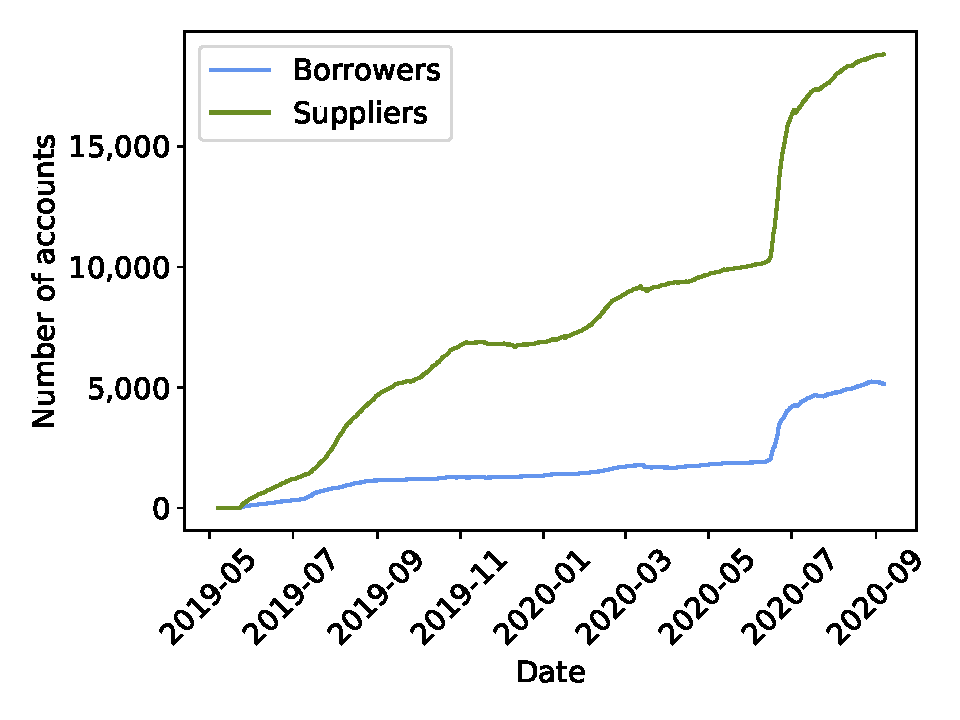
\includegraphics[width=\textwidth]{./5b-economic-security/figures/suppliers-borrowers-over-time.pdf}
    \caption{Number of suppliers and borrowers.}
    \label{fig:borrowers-suppliers-over-time}
  \end{subfigure}
  \begin{subfigure}{.5\textwidth}
    \centering
    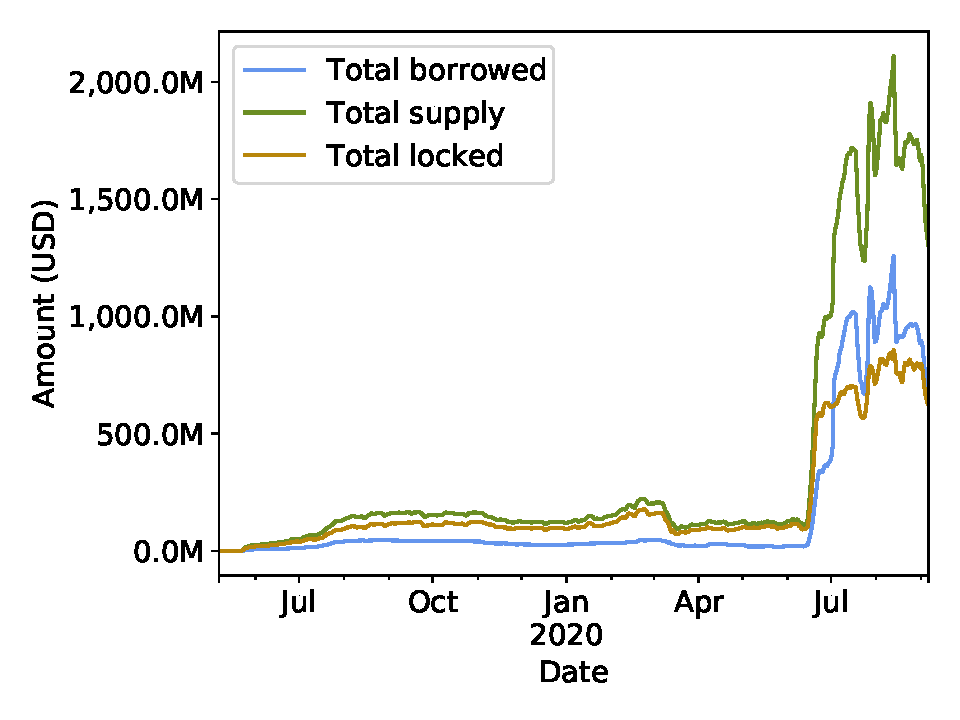
\includegraphics[width=\textwidth]{./5b-economic-security/figures/borrow-supply-over-time.pdf}
    \caption{Amount of funds supplied, borrowed and locked.}
    \label{fig:borrow-supply-over-time}
  \end{subfigure}
  \caption{Number of active accounts and amount of funds on Compound over time.}
\end{figure}

\begin{table}[tbp]
  \centering
  \setlength{\tabcolsep}{5pt}
  \caption{Monitored contracts}
  \label{tab:monitored-contracts}
  \begin{tabular}{l l}
    \toprule
    Name & Address\\
    \midrule
    cBAT & \contractaddr{0x6c8c6b02e7b2be14d4fa6022dfd6d75921d90e4e}\\
    cDAI & \contractaddr{0x5d3a536e4d6dbd6114cc1ead35777bab948e3643}\\
    cETH & \contractaddr{0x4ddc2d193948926d02f9b1fe9e1daa0718270ed5}\\
    cREP & \contractaddr{0x158079ee67fce2f58472a96584a73c7ab9ac95c1}\\
    cSAI & \contractaddr{0xf5dce57282a584d2746faf1593d3121fcac444dc}\\
    cUSDC & \contractaddr{0x39aa39c021dfbae8fac545936693ac917d5e7563}\\
    cUSDT & \contractaddr{0xf650c3d88d12db855b8bf7d11be6c55a4e07dcc9}\\
    cWBTC & \contractaddr{0xc11b1268c1a384e55c48c2391d8d480264a3a7f4}\\
    cZRX & \contractaddr{0xb3319f5d18bc0d84dd1b4825dcde5d5f7266d407}\\
    Comptroller & \contractaddr{0x3d9819210a31b4961b30ef54be2aed79b9c9cd3b}\\
    Open Oracle Price Data & \contractaddr{0x02557a5e05defeffd4cae6d83ea3d173b272c904}\\
    Uniswap Anchored View & \contractaddr{0x9b8eb8b3d6e2e0db36f41455185fef7049a35cae}\\
    \bottomrule
  \end{tabular}
\end{table}

\begin{table}[tbp]
	\caption[Top 10 suppliers and borrowers on Compound]{Top 10 suppliers and borrowers. Amounts are expressed in their USD equivalent. Addresses marked with $\checkmark$ are smart contract addresses, among which the one with the most supplied funds is a Curve pool address that aggregates funds from multiple parties.
		%   and the ``A'' column is checked if it is an \emph{aggregator} (e.g. Curve pool).
	}
	\label{tab:top-suppliers-borrowers}
	\setlength{\tabcolsep}{5pt}
	\begin{subtable}{\textwidth}
		\caption{Top 10 users with the largest amount of funds supplied}
		\begin{tabular}{lcrl}
			\toprule
			\textbf{Address}                                                  &            & \textbf{Amount} & \textbf{Description}    \\
			\midrule
			\contractaddr[\small]{0x554bd2947df1c8d8d38897bdc92b3b97692b2845} &            & 342,128,032     &                         \\
			\contractaddr[\small]{0xa2b47e3d5c44877cca798226b7b8118f9bfb7a56} & \checkmark & 40,284,236      & Curve pool              \\
			\contractaddr[\small]{0x04b0b0e460c9fc583d9c93bc9ae25b353390645e} & \checkmark & 34,908,472      & Instadapp smart wallet  \\
			\contractaddr[\small]{0x25599dcbd434af9a17d52444f71c92987fa97cfc} &            & 34,530,570      &                         \\
			\contractaddr[\small]{0x58485ea7106891bdd94c37ced30c6fdbc5293b16} & \checkmark & 32,686,029      & Multisig wallet         \\
			\contractaddr[\small]{0x909b443761bbd7fbb876ecde71a37e1433f6af6f} &            & 29,308,425      &                         \\
			\contractaddr[\small]{0xea61f3052753ea2c6a1c208583ad9b0394ed2f28} & \checkmark & 28,854,366      & DeFi Saver smart wallet \\
			\contractaddr[\small]{0x32b2d4ec46d76fc6dabfe958fb0e0bd8db740c84} &            & 27,928,637      &                         \\
			\contractaddr[\small]{0xedcc13d25e23032b61d30c298334f92d7c0ba84e} &            & 27,709,153      &                         \\
			\contractaddr[\small]{0x6d2af065ccb60c0f7e8ec5907c961c42a3447127} &            & 25,559,037      &                         \\
			\bottomrule
		\end{tabular}
	\end{subtable}
	\begin{subtable}{\textwidth}
		\caption{Top 10 users with the largest amount of funds borrowed}
		\begin{tabular}{llrl}
			\toprule
			\textbf{Address}                                                  &            & \textbf{Amount} & \textbf{Description}    \\
			\midrule
			\contractaddr[\small]{0x554bd2947df1c8d8d38897bdc92b3b97692b2845} &            & 247,143,532     &                         \\
			\contractaddr[\small]{0x25599dcbd434af9a17d52444f71c92987fa97cfc} &            & 22,085,613      &                         \\
			\contractaddr[\small]{0x909b443761bbd7fbb876ecde71a37e1433f6af6f} &            & 21,030,095      &                         \\
			\contractaddr[\small]{0x58485ea7106891bdd94c37ced30c6fdbc5293b16} & \checkmark & 20,149,687      & Multisig wallet         \\
			\contractaddr[\small]{0x32b2d4ec46d76fc6dabfe958fb0e0bd8db740c84} &            & 18,900,729      &                         \\
			\contractaddr[\small]{0xea61f3052753ea2c6a1c208583ad9b0394ed2f28} & \checkmark & 18,248,324      & DeFi Saver smart wallet \\
			\contractaddr[\small]{0xedcc13d25e23032b61d30c298334f92d7c0ba84e} &            & 17,643,172      &                         \\
			\contractaddr[\small]{0x6d2af065ccb60c0f7e8ec5907c961c42a3447127} &            & 12,015,576      &                         \\
			\contractaddr[\small]{0x79dbd1baf124edd4205b2aba56c29bf3914c8ed0} &            & 11,632,820      &                         \\
			\contractaddr[\small]{0x0c8a8dd439069690a5722d5fbb18359a68e279f1} &            & 10,009,553      &                         \\
			\bottomrule
		\end{tabular}
	\end{subtable}
\end{table}


\subsection{Analysis}
\label{sec:5b:analysis}
In this section, we present the results of the analysis performed with the framework outlined in \autoref{sec:5b:methodology}.
We analyze data from the Compound protocol~\cite{leshner2018} over a period ranging from \StartDate---when the first Compound markets were deployed on the Ethereum main network---to \EndDate.
In \autoref{tab:monitored-contracts}, we provide a list of contracts we monitored in our analysis.
When analysing a single market, we choose the market for \coin{DAI}, as it is the largest by an order of magnitude.

\begin{figure}[tbp]
  \begin{subfigure}{.5\textwidth}
    \centering
    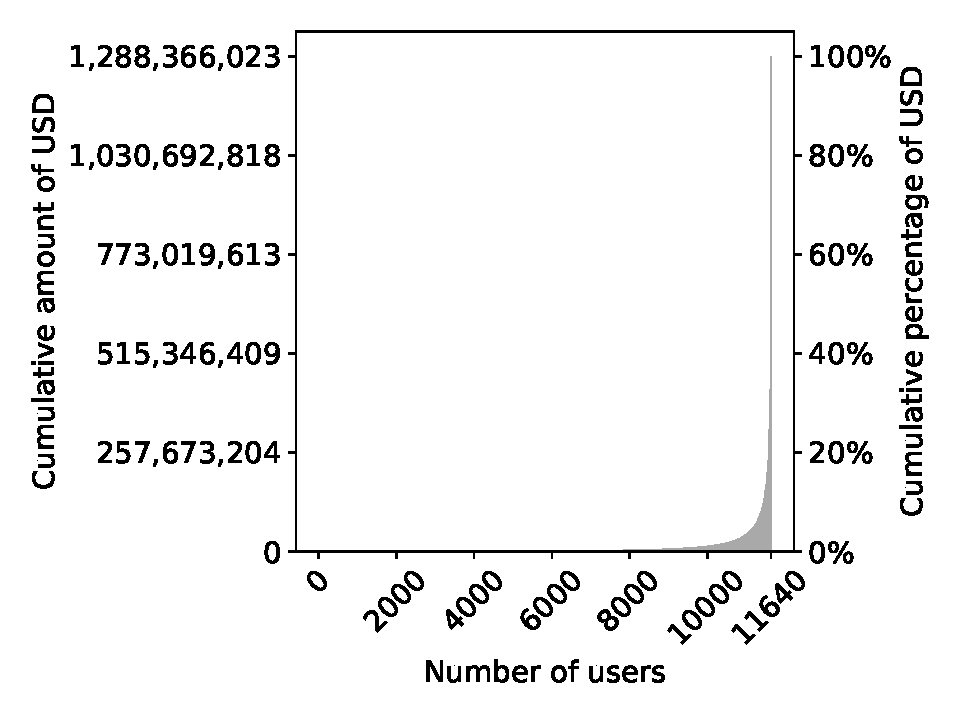
\includegraphics[width=\textwidth]{./5b-economic-security/figures/suppliers-distribution.pdf}
    \caption{Distribution of supplied funds.}
    \label{fig:suppliers-distribution}
  \end{subfigure}
  \begin{subfigure}{.5\textwidth}
    \centering
    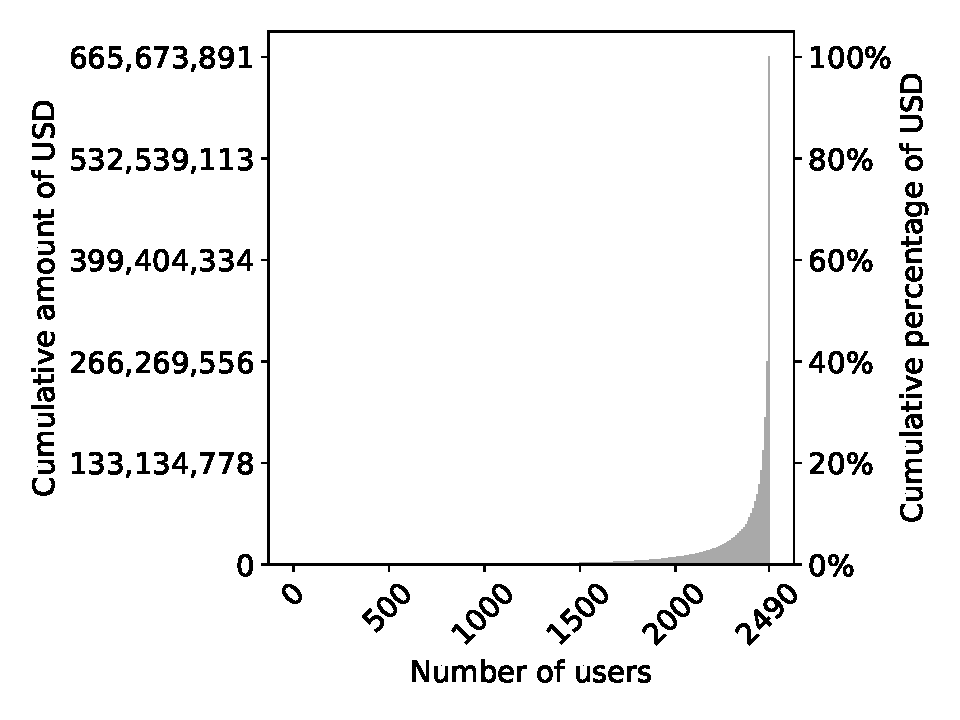
\includegraphics[width=\textwidth]{./5b-economic-security/figures/borrowers-distribution.pdf}
    \caption{Distribution of borrowed funds.}
    \label{fig:borrowers-distribution}
  \end{subfigure}
  \caption[Cumulative distribution of funds in USD on Compound]{Cumulative distribution of funds in USD.~Accounts are sorted from least to most wealthy and bucketed in bins of 10, i.e. a single bar represents the sum of 10 accounts.}\label{fig:suppliers-borrowers-distribution}
\end{figure}


\subsubsection{Borrowers and Suppliers}
We first examine the total number of borrowers and suppliers on Compound by considering any Ethereum account that, at any time within the observation period, either exhibited a non-zero cToken balance or borrowed funds for any Compound market.
The change in the number of borrowers and suppliers over time is displayed in \autoref{fig:borrowers-suppliers-over-time}.

We see that the total number of suppliers always exceeds the total number of borrowers. 
This is because on Compound, one can only borrow against funds he supplied as collateral, which automatically makes the borrower also a supplier. 
Interestingly, the number of suppliers has increased relative to the number of borrowers over time. 
There is a notable sudden jump in both the number of suppliers and borrowers in June~2020.

In terms of total deposits, a very similar trend is observable in \autoref{fig:borrow-supply-over-time}, which shows that at the same time, the total supplied deposits increased, while the total borrows followed shortly after.
Furthermore, the total funds borrowed exceeded the total funds locked for the first time in July 2020 and remained so until the end of the examined period.
We discuss the reasons behind this in the next part of this section.

Despite the similarly increasing trend for the number of suppliers/borrowers and amount of supplied/borrowed funds, we can see in~\autoref{fig:suppliers-borrowers-distribution} that the majority of funds are borrowed and supplied only by a small number of accounts.
For instance, for the suppliers in~\autoref{fig:suppliers-distribution}, the top user and top 10 users supply~27.4\% and~49\% of total funds, respectively.
For the borrowers shown in~\autoref{fig:borrowers-distribution}, the top user accounts for 37.1\%, while the top 10 users account for 59.9\% of total borrows.
While one could think that this concentration comes from the fact that top accounts are pools receiving money from several participants, only one of the top~10 suppliers and none of the top~10 borrowers fit in this category.
In~\autoref{tab:top-suppliers-borrowers}, we show the top 10 suppliers and borrowers in terms of the total amount borrowed and supplied expressed in USD.
We mark the addresses that are smart contracts. Among those contracts, the one with the most supplied funds, \contractaddr[\scriptsize]{0xa2b47e3d5c44877cca798226b7b8118f9bfb7a56}, is the address of a Curve~\cite{web:curve} pool that has funds coming from several independent parties.
No other address among top suppliers and borrowers is a pool address.


\subsubsection{Leveraging Spirals}
As we have seen in \autoref{sec:5b:plfs}, in PLFs, leveraging can be used either to gain more exposure to a particular currency or to gain some incentive provided by the protocol.
To understand how leveraging can affect the total amounts borrowed and supplied on Compound, we use the methodology we defined in \autoref{ssec:leveraging-spirals-meth} to measure the existence of leveraging spirals on Compound.

We find that the top supplier deposited a total of 342 million USD and borrowed 247 million.
However, after the inspection of leveraging spirals, we find that the user has provided only 16\% of the funds, while the rest of the minted funds have been part of leveraging spirals, which means that the user provided a total of roughly 55 million USD to the protocol.

In total, we find a total of 2,141 accounts using this leveraging spiral technique for a total of over 600 million USD, or roughly half of the total amount of funds supplied to the protocol.

\subsubsection{The \coin{COMP} Governance Token}
The sudden jumps exhibited in \autoref{fig:borrowers-suppliers-over-time} and \autoref{fig:borrow-supply-over-time} can be explained by the launch of Compound's governance token, \coin{COMP}, on June~15,~2020.
The \coin{COMP} governance token allows holders to participate in voting, create proposals, as well as delegate voting rights.
In order to empower Compound stakeholders, new \coin{COMP} is minted every block and distributed among borrowers and suppliers in each market.

Initially, \coin{COMP} was allocated proportionally to the accrued interest per market.
However, the \coin{COMP} distribution model was modified via a governance vote on July~2,~2020, such that the borrowing interest rate was removed as a weighting mechanism in favour of distributing \coin{COMP} per market on a borrowing demand basis, i.e.\ per USD borrowed.
The distributed \coin{COMP} per market is shared equally between a market's borrowers and suppliers, who receive \coin{COMP} proportionally to their borrowed and supplied amounts, respectively.
Hence, a Compound user is incentivized to increase his borrow position as long as the borrowing cost does not exceed the value of his \coin{COMP} earnings. This presumably explains the drop in the degree of collateralization, as the total amount locked is seen surpassed by the total borrows after the \coin{COMP} launch (\autoref{fig:borrow-supply-over-time}), leading to elevated liquidation risk of borrow positions.


\begin{figure}[tbp]
  \centering
  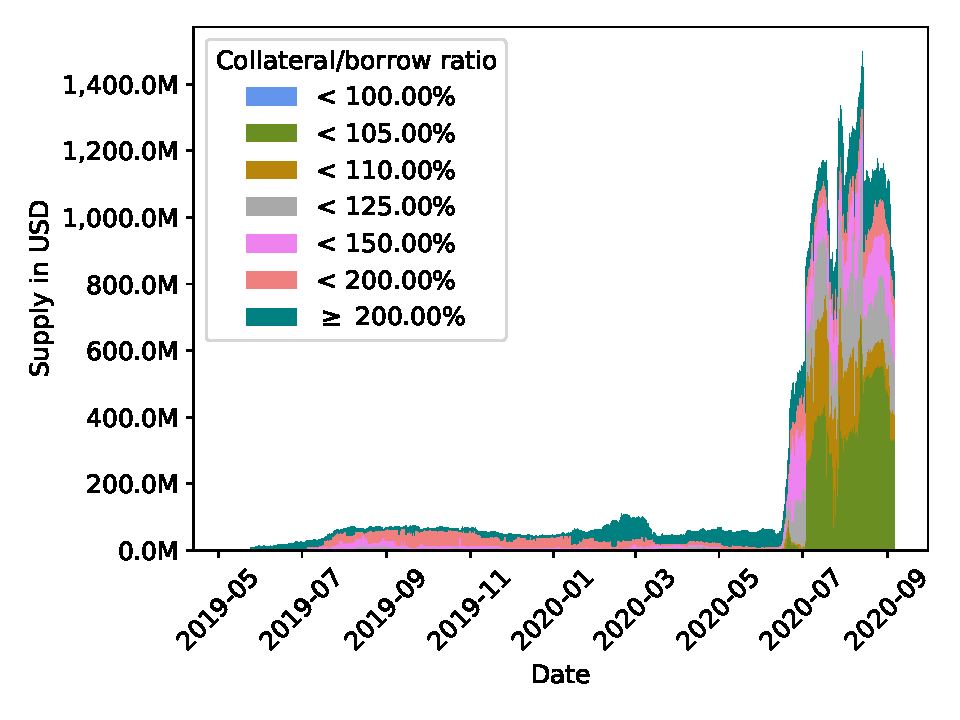
\includegraphics[width=0.7\textwidth]{./5b-economic-security/figures/supply-borrow-over-time.pdf}
  \caption[Collateral locked on Compound over time]{Collateral locked over time, showing how close the amounts are from being liquidated. Positions can be liquidated when the ratio drops below~100\%.}
  \label{fig:liquidatability}
\end{figure}

\subsubsection{Liquidation Risk}
Given the high increase in the number of total funds borrowed and supplied, as well as the decrease in liquidity relative to total borrows, we seek to identify and quantify any changes in liquidation risk on Compound since the launch of \coin{COMP}. 
\autoref{fig:liquidatability} shows the total USD value of collateral on Compound and how close collateral amounts are to liquidation. 
In addition to the substantial increase in the total value of collateral on Compound since the launch of \coin{COMP}, the risk-seeking behaviour of users has also changed.
This can be seen by examining collateral-to-borrow ratios, where since the beginning of July,~2020, a total of approximately 350m to 600m USD worth of collateral has been within a 5\% price range of becoming liquidatable.
However, it should be noted that the likelihood of the amount of this collateral becoming liquidatable highly depends on the price volatility of the collateral asset.

In order to examine how liquidation risk differs across markets, we measure for the largest market on Compound, namely \coin{DAI}, the sensitivity of collateral becoming liquidatable given a decrease in the price of \coin{DAI}.
\autoref{fig:price-sensitivity} shows the amount of aggregate collateral liquidatable at the historic price, as well as at a~3\% and~5\% decrease relative to the historic price for \coin{DAI}.
We mark the date on which the \coin{COMP} governance token launched with a dashed line.
It can be seen that since the launch of \coin{COMP},~3\% and~5\% price decreases of \coin{DAI} relative to its peg USD would have resulted in a substantially higher amount of liquidatable collateral.
In particular, a~3\% decrease would have turned collateral worth in excess of~10 million USD liquidatable.

\begin{figure}[tb]
  \centering
  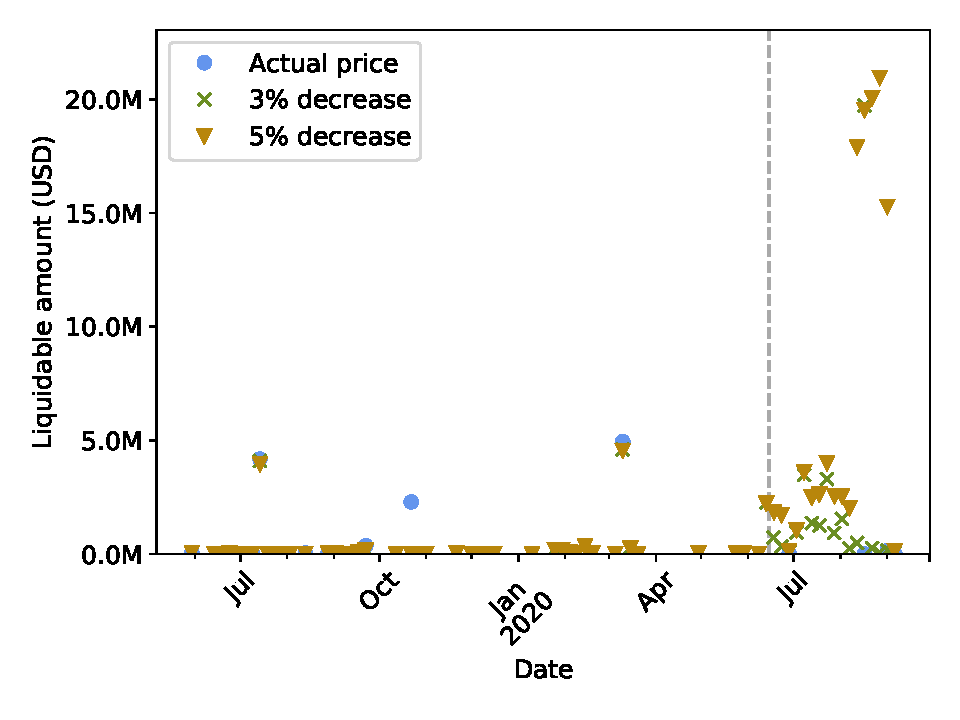
\includegraphics[width=.7\textwidth]{./5b-economic-security/figures/dai-sensitivity.pdf}
  \caption[Sensitivity analysis of the liquidatable collateral amount]{Sensitivity analysis of the liquidatable collateral amount given \coin{DAI} price movement relative to its peg USD. \coin{COMP} launch date is marked by the dashed vertical line.}
  \label{fig:price-sensitivity}
\end{figure}

\begin{figure}[tb]
  \centering
  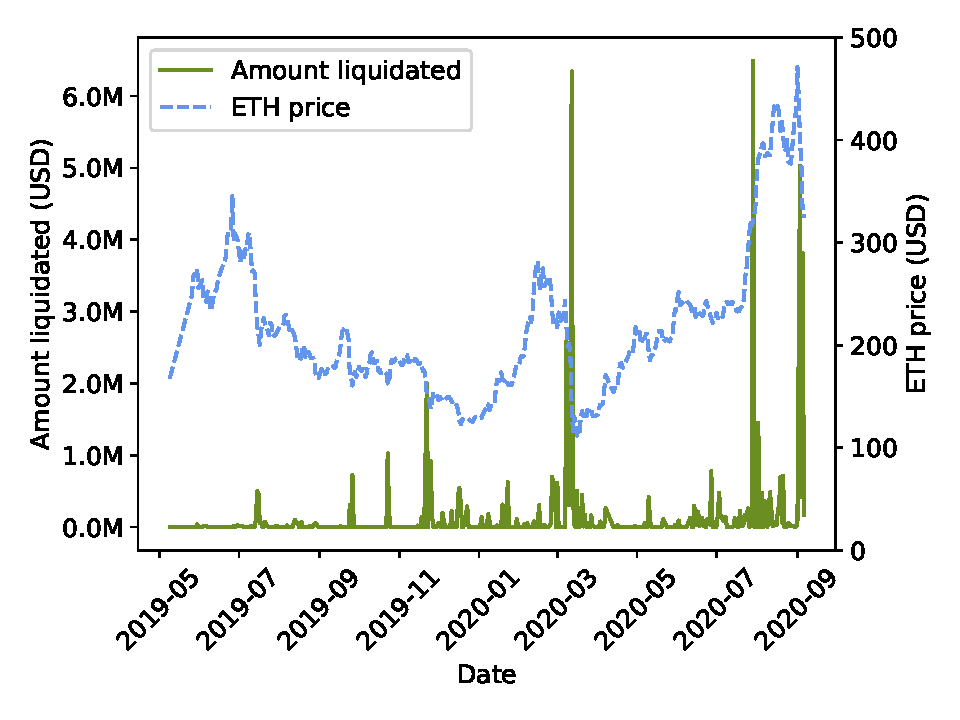
\includegraphics[width=.7\textwidth]{./5b-economic-security/figures/liquidation-over-time.pdf}
  \caption{Amount (in USD) of liquidated collateral from May ~2019 to August 2020.}
  \label{fig:liquidations-over-time}
\end{figure}

\subsubsection{Liquidations and Liquidators}
In order to better understand the implications of the increased liquidation risk since the launch of \coin{COMP}, we examine historical liquidations on Compound and subsequently measure the efficiency of liquidators.

\point{Historical Liquidations}
The increased risk-seeking behaviour suggested by the low collateral-to-borrow ratios presented in the previous section are in accordance with the trend of rising amount of liquidated collateral since the introduction of \coin{COMP}.  
The total value of collateral liquidated on Compound over time is shown in \autoref{fig:liquidations-over-time}.
It can be seen that the majority of this collateral was liquidated on a few occasions, perhaps most notably on Black Thursday (March 12, 2020), July 29, 2020 (\coin{DAI} deviating from its peg significantly), and in early September 2020 (\coin{ETH} price drop).

\point{Liquidation Efficiency}
We measure the efficiency of liquidators as the number of blocks elapsed since a borrow position has become liquidatable and the position actually being liquidated.
The overall historical efficiency of liquidators is shown as a cumulative distribution function in \autoref{fig:blocks-spent}, from which it can be seen that approximately~60\% of the total liquidated collateral (35 million USD) was liquidated within the same block as it became liquidatable, suggesting that the majority of liquidations occur via bots in a highly efficient fashion.
After~2 blocks have elapsed (on average half a minute),~85\% of liquidatable collateral has been liquidated, and after 16 blocks this value amounts to~95\%.

It is worth noting that liquidation efficiency has been skewed by the more recent liquidation activities which were of a much larger scale than when the protocol was first launched.
Specifically, in 2019, only about~26\% of the liquidations occurred in the block during which the position became liquidatable, compared to~70\% in 2020.
This resulted in some lost opportunities for liquidators as shown in~\autoref{fig:price-sensitivity}.
The account \contractaddr{0xd062eeb318295a09d4262135ef0092979552afe6}, for instance, had more than 3,000,000 USD worth of \coin{ETH} as collateral exposed at block 8,796,900 for the duration of a single block: the account was roughly 20 USD shy of the liquidation threshold but eventually escaped liquidation.
If a liquidator had captured this opportunity, he could have bought half of this collateral (given the close factor of 0.5), at a 10\% discount, resulting in a profit of 150,000 USD for a single transaction.
It is clear that with such stakes, participants were incentivized to improve liquidation techniques, resulting in a high level of liquidation speed and scale.

\begin{figure}[tbp]
    \centering
    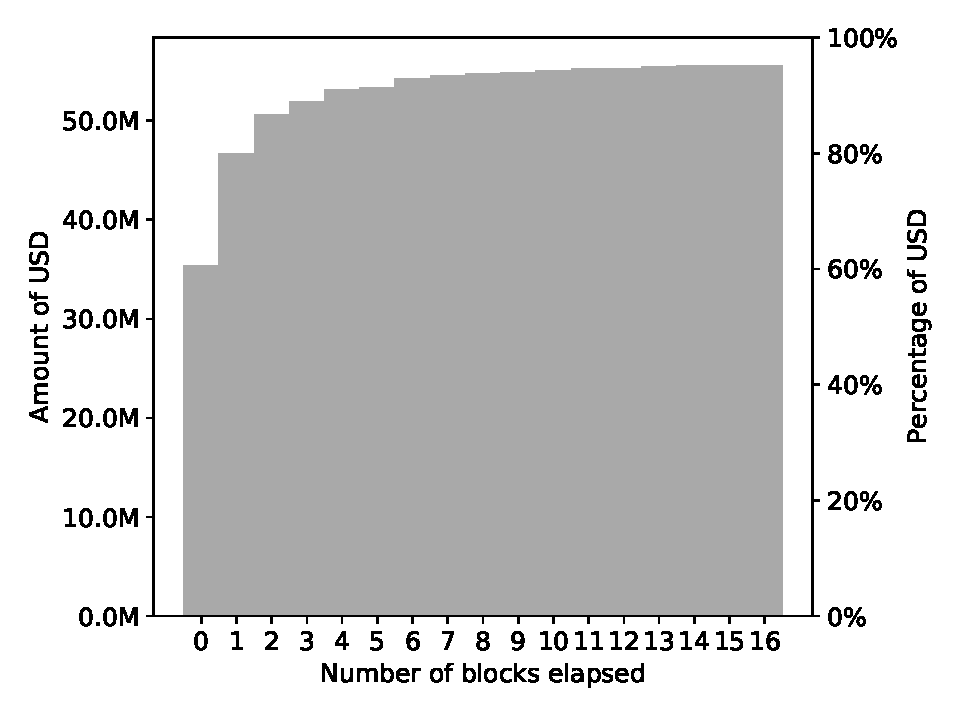
\includegraphics[width=0.7\textwidth]{./5b-economic-security/figures/time-to-liquidation.pdf}
    \caption[Number of blocks elapsed until liquidation]{Number of blocks elapsed from the time a position can be liquidated to actual liquidation on Compound from \StartDate to \EndDate, shown as a CDF.}
    \label{fig:blocks-spent}
\end{figure}

\subsubsection{Summary}
In this section, we have analysed the Compound protocol with a focus on liquidations.
We have found that despite the increase in the number of suppliers and borrowers over time, the total amount of funds supplied and borrowed remained extremely concentrated among a small set of participants.

We have also seen that the introduction of the \coin{COMP} governance token has changed how users interact with the protocol and the amount of risk that they are willing to take.
Users now borrow vastly more than before, with the total amount borrowed surpassing the total amount locked.
Due to excessive borrowing without a sufficiently safe amount of supplied funds, borrow positions now face a higher liquidation risk, such that a crash of~3\% in the price of \coin{DAI} could result in an aggregate liquidation value of over~10 million USD.

Finally, we have shown that the liquidators have become more efficient with time, and are currently able to capture a majority of the liquidatable funds instantly.


\subsection{Discussion}
\label{sec:discussion}
In this section, we enumerate several points that we deem important for the future development of PLFs and DeFi protocols.
We first discuss the influence of governance tokens, by intention or not, on how users behave within a protocol.
Subsequently, we discuss potential risks that lie in the use of governance tokens, and the contagion effect that user behavior in a protocol can have on another protocol.
Finally, we discuss how miner-extractable value~\cite{daian2020flash} can potentially affect liquidation incentives in such protocols.

\subsubsection{Governance Token Influence}
As analyzed in Section~\ref{sec:analysis}, the distribution of the \coin{COMP} token has vastly changed the Compound landscape and user behavior.
Until the introduction of the token, borrowing was costly due to the payable interest, which implies a negative cash flow for the borrower. Therefore, a borrower would only borrow if he could justify this negative cash flow with some application external to Compound.
With the introduction of this token, borrowing could yield a positive cash flow due to the monetary value of the governance token.
This creates a situation where both suppliers and borrowers end up with a positive cash flow, inducing users to maximize both their supply and borrow.
This model is, however, only sustainable when the price of the \coin{COMP} token remains sufficiently high to keep this cash flow positive for borrowers.
This directly results in users taking increasingly higher risk in an attempt to gain larger monetary rewards, with liquidators ultimately profiting more from their operations.

\subsubsection{Governance Token Risks}
The increased use of governance tokens across DeFi protocols (e.g. \coin{YFI} on Yearn Finance, \coin{AAVE} on Aave, \coin{UNI} on Uniswap) can be seen as a promising step towards achieving a higher degree of decentralization in terms of protocol governance. 
However, despite the increased usage of governance tokens, to the best of our knowledge there is still a dearth of academic research examining the different governance models and specifically the relation between their security assumptions and the employed governance token.
For instance, the option to aggregate governance tokens via flash loans \cite{Wang2020} can pose a significant security risk to DeFi protocols should an attacker attempt to propose and execute malicious protocol updates.
Furthermore, even in the case of flash loan resistant governance models, the relationship between the financial value of a protocol's governance token and the economically secure regions of the protocol remains unexamined and serves as a further risk that designers of governance models have to take into account.
Despite the existence of protective mechanisms against governance attacks on some protocols (e.g. multi-sig approvals or selected ``guardians'' that are able to halt the governance process), it remains questionable which of such mechanisms are indeed desirable from a decentralized governance perspective and whether there might be more suitable alternatives.

\subsubsection{Contagion Effects}
This behavior also indirectly affected other protocols, in particular \coin{DAI}.
The price of \coin{DAI} is aimed to be pegged to 1 USD resting on an arbitrage mechanism, whereby token holders are incentivized to buy or sell \coin{DAI} as soon as the price moves below or above 1 USD, respectively.
However, a rational user seeking to maximize profit will not sell his \coin{DAI} if holding it somewhere else would yield higher profits.
This was precisely what was happening with Compound, whose users locking their \coin{DAI} received higher yields in the form of \coin{COMP}, than from selling \coin{DAI} at a premium, thereby resulting in upward price pressure~\cite{cyrus2020upcoming}.
Interestingly, \coin{DAI} deviating from its peg also has a negative effect for Compound users.
Indeed, as we saw in Section~\ref{sec:analysis}, many Compound users might have been overconfident about the price stability of \coin{DAI} and thus only collateralize marginally above the threshold when they borrow \coin{DAI}.
This has resulted in large amounts being liquidated due to the actual, higher extent of the volatility in the \coin{DAI} price.

\subsubsection{Miner-Extractable Value}
In the context of PLFs, liquidations can be seen as miner-extractable value.
Indeed, it is easy for the miner to check whether a position is liquidable or not after each processed transaction and to add a transaction to liquidate the position immediately after the transaction making it liquidable.
In our analysis of the Compound protocol, we have not found any sign of miners participating in liquidations, directly or indirectly.
We show the top miners and the top liquidators for each miner in~\autoref{tab:miners-liquidators} of Appendix~\ref{sec:miners-liquidators}.
Although we found no correlation between miners and liquidators, this is a real risk that could make the role of liquidator, which is essential for the protocol security, less interesting for those who are not collaborating with miners.


\subsection{Related Work}
\label{sec:5b:related-work}

% Almgren and Chriss~\cite{Almgren1999} demonstrate how liquidity and transaction costs can be accounted for in a portfolio theory framework, and describe a valuation model for portfolios under liquidation.

% Ramcharan~\cite{Ramcharan2020} examine the liquidation with banks and finds that lower bank equity or liquidity results in lower liquidation value of band-owned real estate collateral.

% Chan and Thakor~\cite{CHAN1987} theorize the equilibria of credit rationing, a phenomenon where lenders limit their supply of credit to borrowers. They find that unlimited collateral may or may not eliminate credit rationing, depending on how a competitive equilibrium is conceptualized.

% Oehmke~\cite{Oehmke2014} model collateral liquidations upon default of a repo borrower, and suggest repo lenders consider their balance set constraints when executing collateral sell-offs.

% Vig~\cite{Vig2013} find that the demand for collateralized debt decreases while the supply increases when the rights of creditors are strengthened. In the same vein, Hall~\cite{Hall2012} find that the high transferability of collateral results in a tighter linkage between leverage and asset tangibility (fixed assets as a fraction of total assets).

% Through an array of case studies, Mann~\cite{Mann2005} discover that in the case of distressed loans, lenders rarely take possession of the collateral, but rather seek to be repaid through either refinancing or sale of the collateral.

% John~\cite{John1993} finds strong empirical evidence for a positive correlation between the liquidity level maintained by an entity and its cost of liquidity, that is, entities with high financial distress costs tend to reduce their exposure to liquidity risks through a lower leverage ratio.

% De Souza and Smirnov~\cite{DeSouza2004} describe the notion of dynamic leverage for investment funds, where the size of leverage should be adjusted depending on the fund equity size, risk-adjusted return targets and investment horizon.


% Schleifer and Vishny~\cite{Shleifer2010}
% Fabbri and Menichini~\cite{Fabbri2010} 

In this section, we briefly discuss existing related work.

A thorough analysis of the Compound protocol with respect to market risks faced by participants was done by~\cite{kao2020}.
The authors employ agent-based modelling and simulation to perform stress tests in order to show that Compound remains safe under high volatility scenarios and high levels of outstanding debt.
Furthermore, the authors demonstrate the potential of Compound to scale to accommodate a larger borrow market while maintaining a low default probability.
This differs from our work as we conduct a detailed empirical analysis of Compound, focusing on how agent behaviour under different incentive structures on Compound has affected the protocol's state with regard to liquidation risk.  

A first in-depth analysis of PLFs is given by~\cite{10.1145/3419614.3423254}.
The authors provide a taxonomy of interest rate models employed by PLFs, while also discussing market liquidity, efficiency and interconnectedness across PLFs.
As part of their analysis, the authors examine the cumulative percentage of locked funds solely for the Compound markets \coin{DAI}, \coin{ETH}, and \coin{USDC}.

In~\cite{bartoletti2020sok}, the authors provide a formal state transition model of PLFs\footnote{Note that in \cite{bartoletti2020sok}, PLFs are referred to as lending pools.} and prove fundamental behavioural properties of PLFs, which had previously only been presented informally in the literature.
Additionally, the authors examine attack vectors and risks, such as utilization attacks and interest-bearing derivative token risks. 
This work differs from our work, as the authors of~\cite{bartoletti2020sok} formalize the properties of PLFs through an abstract model, while we provide a thorough empirical analysis with a focus on liquidations and risks brought upon by governance tokens, such as for Compound and the \coin{COMP} token.

In \cite{klages2019stability}, the authors show how markets for stablecoins are exposed to deleveraging feedback effects, which can cause periods of illiquidity during a crisis.

The authors of \cite{gudgeon2020decentralized} demonstrate how various DeFi lending protocols are subject to different attack vectors such as governance attacks and under-collateralization.
In the context of the proposed governance attack, the lending protocol the authors focus on is Maker~\cite{whitepaper:maker}.

% Add SoK on lending pools


% Clack and Vanca~\cite{Clack2018} maintain that for a rigorous design of smart contracts for financial derivatives, it is crucial to have a thorough comprehension of the intricacies of conventional legal contracts. They propose a framework for semantic analysis of conventional legal contracts for financial derivatives.

% Chen and Bellavitis~\cite{Chen2020} acknowledge that blockchain technology disrupts the financial industry, while also presenting risks that DeFi as a new form of financial service is associated with, including fraud, volatility and regulatory uncertainty.

% Similarly, Zetzsche~\cite{Zetzsche2020} argue that DeFi is susceptible to cyberattacks facilitated by tech-monoculture and an increased number of access points to the network.


\subsection{Conclusion}
\label{sec:conclusion}
In this section, we presented the first in-depth empirical analysis of liquidations on Compound, one of the largest PLFs in terms of total locked funds, from~\StartDate to~\EndDate.
We analyzed agents' behavior and in particular how much risk they are willing to take within the protocol.
Furthermore, we assessed how this has changed with the launch of the Compound governance token \coin{COMP}, where we found that agents take notably higher risks in anticipation of higher earnings.
This resulted in variations as little as 3\% in an asset's price being able to turn over 10 million USD worth of collateral liquidable.
In order to better understand the potential consequences, we then measured the efficiency of liquidators, namely how quickly new liquidation opportunities are captured. Liquidators' efficiency was found to have improved significantly over time, reaching 70\% of instant liquidations.
Lastly, we demonstrated how overconfidence in the price stability of \coin{DAI}, increased the overall liquidation risk faced by Compound users.
Rather ironically, many users wishing to make the most of the new incentive scheme ended up causing higher volatility in \coin{DAI}---a dominant asset of the platform, resulting in liquidation of their own assets.
This is not Compound's misdoing, but rather highlights the to date unknown dynamics of incentive structures across different DeFi protocols.


\subsection{Monitored Contracts}
\label{sec:monitored-contracts}
In \autoref{fig:monitored-contracts}, we provide a list of contracts we monitored in our analysis.

\begin{figure}[h!]
  \centering
  \setlength{\tabcolsep}{5pt}
  \begin{tabular}{l l}
    \toprule
    Name & Address\\
    \midrule
    cBAT & \contractaddr{0x6c8c6b02e7b2be14d4fa6022dfd6d75921d90e4e}\\
    cDAI & \contractaddr{0x5d3a536e4d6dbd6114cc1ead35777bab948e3643}\\
    cETH & \contractaddr{0x4ddc2d193948926d02f9b1fe9e1daa0718270ed5}\\
    cREP & \contractaddr{0x158079ee67fce2f58472a96584a73c7ab9ac95c1}\\
    cSAI & \contractaddr{0xf5dce57282a584d2746faf1593d3121fcac444dc}\\
    cUSDC & \contractaddr{0x39aa39c021dfbae8fac545936693ac917d5e7563}\\
    cUSDT & \contractaddr{0xf650c3d88d12db855b8bf7d11be6c55a4e07dcc9}\\
    cWBTC & \contractaddr{0xc11b1268c1a384e55c48c2391d8d480264a3a7f4}\\
    cZRX & \contractaddr{0xb3319f5d18bc0d84dd1b4825dcde5d5f7266d407}\\
    Comptroller & \contractaddr{0x3d9819210a31b4961b30ef54be2aed79b9c9cd3b}\\
    Open Oracle Price Data & \contractaddr{0x02557a5e05defeffd4cae6d83ea3d173b272c904}\\
    Uniswap Anchored View & \contractaddr{0x9b8eb8b3d6e2e0db36f41455185fef7049a35cae}\\
    \bottomrule
  \end{tabular}
  \caption{Monitored contracts}
  \label{fig:monitored-contracts}
\end{figure}

\subsection{Top Suppliers and Borrowers}
\label{sec:top-suppliers-borrowers}
In~\autoref{tab:top-suppliers-borrowers}, we show the top 10 suppliers and borrowers in terms of amount borrowed and supplied expressed in USD.
We mark the addresses that are smart contracts. Among those contracts, the one with the most supplied funds, \contractaddr[\scriptsize]{0xa2b47e3d5c44877cca798226b7b8118f9bfb7a56}, is the address of a Curve~\cite{web:curve} pool that has funds coming from a several independent parties.
No other address among top suppliers and borrowers is a pool address.

\subsection{Relationship Between Miners and Liquidators}
\label{sec:miners-liquidators}
In~\autoref{tab:miners-liquidators}, we show the 10 miners who mined the most blocks containing at least one liquidation.
For each miner, we show the 5 liquidators who liquidated the most positions in blocks mined by the given miner.
Overall, we see that for every miner, the liquidations are spread relatively evenly across the different liquidators.
Although we only show the top 10 miners for space constraints, we noted that this was the case for all miners in our dataset.


\hypersetup{hidelinks}

\renewcommand{\contractaddr}[2][\ssmall]{{#1\href{https://etherscan.io/token/#2}{\texttt{#2}}}}
\begin{figure}
	%   \setlength{\tabcolsep}{0.6pt}
	\scriptsize
	\renewcommand{\arraystretch}{1.2}
	\begin{tabular}{@{}l@{}rl@{}r@{}}
		\toprule
		\textbf{Miner}                                                             & \textbf{Blocks}       & \textbf{Liquidators}                                      & \textbf{Liquidations} \\
		                                                                           & \textbf{count}        &                                                           & \textbf{count}        \\
		\midrule
		\multirow{5}{*}{\contractaddr{0x5A0b54D5dc17e0AadC383d2db43B0a0D3E029c4c}} & \multirow{5}{*}{1281} & \contractaddr{0x6a0c50788E462f322959A2458687096994d66316} & 144                   \\
		                                                                           &                       & \contractaddr{0x8c863333c2E92f02e01F7A3c6d131E4d59f78990} & 114                   \\
		                                                                           &                       & \contractaddr{0x0c31b6605686aa26df47eb45AF0e4aa6639A5fd6} & 91                    \\
		                                                                           &                       & \contractaddr{0xb00ba6778cF84100da676101e011B3d229458270} & 76                    \\
		                                                                           &                       & \contractaddr{0x268a1b7ECC1fE1FaB1eE32a7e61e3b7810BAD4a5} & 70                    \\
		\hline
		\multirow{5}{*}{\contractaddr{0xEA674fdDe714fd979de3EdF0F56AA9716B898ec8}} & \multirow{5}{*}{969}  & \contractaddr{0x6a0c50788E462f322959A2458687096994d66316} & 88                    \\
		                                                                           &                       & \contractaddr{0xb00ba6778cF84100da676101e011B3d229458270} & 75                    \\
		                                                                           &                       & \contractaddr{0x8c863333c2E92f02e01F7A3c6d131E4d59f78990} & 70                    \\
		                                                                           &                       & \contractaddr{0x0c31b6605686aa26df47eb45AF0e4aa6639A5fd6} & 52                    \\
		                                                                           &                       & \contractaddr{0x268a1b7ECC1fE1FaB1eE32a7e61e3b7810BAD4a5} & 50                    \\
		\hline
		\multirow{5}{*}{\contractaddr{0x829BD824B016326A401d083B33D092293333A830}} & \multirow{5}{*}{310}  & \contractaddr{0x6a0c50788E462f322959A2458687096994d66316} & 31                    \\
		                                                                           &                       & \contractaddr{0x8c863333c2E92f02e01F7A3c6d131E4d59f78990} & 26                    \\
		                                                                           &                       & \contractaddr{0x402a75f3500CA1FbA17741Ec916F07a0c9DB195D} & 23                    \\
		                                                                           &                       & \contractaddr{0xb00ba6778cF84100da676101e011B3d229458270} & 18                    \\
		                                                                           &                       & \contractaddr{0x029720A9b3CE72f3e1D9C79257E1F19AfE20b6c9} & 17                    \\
		\hline
		\multirow{5}{*}{\contractaddr{0x52bc44d5378309EE2abF1539BF71dE1b7d7bE3b5}} & \multirow{5}{*}{257}  & \contractaddr{0x6a0c50788E462f322959A2458687096994d66316} & 22                    \\
		                                                                           &                       & \contractaddr{0x10aab4B0EF76AA2AC9b5909e671517a1171B050E} & 21                    \\
		                                                                           &                       & \contractaddr{0x8c863333c2E92f02e01F7A3c6d131E4d59f78990} & 16                    \\
		                                                                           &                       & \contractaddr{0x402a75f3500CA1FbA17741Ec916F07a0c9DB195D} & 15                    \\
		                                                                           &                       & \contractaddr{0x0006e4548AED4502ec8c844567840Ce6eF1013f5} & 14                    \\
		\hline
		\multirow{5}{*}{\contractaddr{0x04668Ec2f57cC15c381b461B9fEDaB5D451c8F7F}} & \multirow{5}{*}{185}  & \contractaddr{0x8c863333c2E92f02e01F7A3c6d131E4d59f78990} & 22                    \\
		                                                                           &                       & \contractaddr{0x5DAfafbd7AcD662C909a9601120cf1D9F277e8aE} & 14                    \\
		                                                                           &                       & \contractaddr{0x10aab4B0EF76AA2AC9b5909e671517a1171B050E} & 14                    \\
		                                                                           &                       & \contractaddr{0x268a1b7ECC1fE1FaB1eE32a7e61e3b7810BAD4a5} & 12                    \\
		                                                                           &                       & \contractaddr{0x6a0c50788E462f322959A2458687096994d66316} & 12                    \\
		\hline
		\multirow{5}{*}{\contractaddr{0xb2930B35844a230f00E51431aCAe96Fe543a0347}} & \multirow{5}{*}{77}   & \contractaddr{0x10aab4B0EF76AA2AC9b5909e671517a1171B050E} & 8                     \\
		                                                                           &                       & \contractaddr{0x0c31b6605686aa26df47eb45AF0e4aa6639A5fd6} & 8                     \\
		                                                                           &                       & \contractaddr{0x5DAfafbd7AcD662C909a9601120cf1D9F277e8aE} & 6                     \\
		                                                                           &                       & \contractaddr{0xf8E562f4F30c5DdA0978857067D6585265dA3437} & 6                     \\
		                                                                           &                       & \contractaddr{0xfDe817C7a0770f42fb80B93dd7A538291C871765} & 5                     \\
		\hline
		\multirow{5}{*}{\contractaddr{0xD224cA0c819e8E97ba0136B3b95ceFf503B79f53}} & \multirow{5}{*}{73}   & \contractaddr{0xb00ba6778cF84100da676101e011B3d229458270} & 13                    \\
		                                                                           &                       & \contractaddr{0x8c863333c2E92f02e01F7A3c6d131E4d59f78990} & 8                     \\
		                                                                           &                       & \contractaddr{0x88886841CfCCBf54AdBbC0B6C9cBAceAbec42b8B} & 8                     \\
		                                                                           &                       & \contractaddr{0xfFA7370a03c2a91f5B1847a90750489d05f52Fa9} & 5                     \\
		                                                                           &                       & \contractaddr{0x492Ff1c96b398297FcAcd6E7E1E968d2b2fc7Da0} & 5                     \\
		\hline
		\multirow{5}{*}{\contractaddr{0x4C549990A7eF3FEA8784406c1EECc98bF4211fA5}} & \multirow{5}{*}{68}   & \contractaddr{0xb00ba6778cF84100da676101e011B3d229458270} & 12                    \\
		                                                                           &                       & \contractaddr{0x6a0c50788E462f322959A2458687096994d66316} & 9                     \\
		                                                                           &                       & \contractaddr{0x402a75f3500CA1FbA17741Ec916F07a0c9DB195D} & 5                     \\
		                                                                           &                       & \contractaddr{0x10aab4B0EF76AA2AC9b5909e671517a1171B050E} & 4                     \\
		                                                                           &                       & \contractaddr{0x8c863333c2E92f02e01F7A3c6d131E4d59f78990} & 3                     \\
		\hline
		\multirow{5}{*}{\contractaddr{0xEEa5B82B61424dF8020f5feDD81767f2d0D25Bfb}} & \multirow{5}{*}{55}   & \contractaddr{0xb00ba6778cF84100da676101e011B3d229458270} & 7                     \\
		                                                                           &                       & \contractaddr{0x402a75f3500CA1FbA17741Ec916F07a0c9DB195D} & 6                     \\
		                                                                           &                       & \contractaddr{0x8c863333c2E92f02e01F7A3c6d131E4d59f78990} & 5                     \\
		                                                                           &                       & \contractaddr{0x029720A9b3CE72f3e1D9C79257E1F19AfE20b6c9} & 5                     \\
		                                                                           &                       & \contractaddr{0x10aab4B0EF76AA2AC9b5909e671517a1171B050E} & 4                     \\
		\hline
		\multirow{5}{*}{\contractaddr{0x84A0d77c693aDAbE0ebc48F88b3fFFF010577051}} & \multirow{5}{*}{46}   & \contractaddr{0xb00ba6778cF84100da676101e011B3d229458270} & 7                     \\
		                                                                           &                       & \contractaddr{0x0c31b6605686aa26df47eb45AF0e4aa6639A5fd6} & 6                     \\
		                                                                           &                       & \contractaddr{0x6a0c50788E462f322959A2458687096994d66316} & 5                     \\
		                                                                           &                       & \contractaddr{0x5e32f33e261a90FF9fE94230387118945599268c} & 5                     \\
		                                                                           &                       & \contractaddr{0x8c863333c2E92f02e01F7A3c6d131E4d59f78990} & 5                     \\
		\bottomrule
	\end{tabular}
	\caption{Top 10 miners per number of blocks containing at least a liquidation event mined and top 5 liquidators for each miner per number of liquidations}%\label{tab:miners-liquidators}
\end{figure}

\hypersetup{pdfborder={0 0 1}}

% \begin{figure}
%   \setlength{\tabcolsep}{4pt}
%   \begin{tabular}{rlrrr}
%     \toprule
%     \textbf{Rank} &                                           \textbf{Address} & \textbf{Supply} & \textbf{Borrow} & \textbf{Ratio} \\
%     \midrule
%     1 &  \contractaddr{0x554bd2947df1c8d8d38897bdc92b3b97692b2845} &         256.60M &         247.14M &           1.04 \\
%     6 &  \contractaddr{0x909b443761bbd7fbb876ecde71a37e1433f6af6f} &          21.98M &          21.03M &           1.05 \\
%     16 &  \contractaddr{0x0c8a8dd439069690a5722d5fbb18359a68e279f1} &          10.27M &          10.01M &           1.03 \\
%     21 &  \contractaddr{0xc2f61a6eeec48d686901d325cde9233b81c793f3} &           8.48M &           8.21M &           1.03 \\
%     31 &  \contractaddr{0x78f6303f7d49166f2da1bb9c679b675234a645bf} &           5.66M &           5.42M &           1.04 \\
%     36 &  \contractaddr{0xb7904059e7f4863ad9efe7778dbe5f663e379501} &           4.60M &           4.54M &           1.01 \\
%     39 &  \contractaddr{0xd09a6dd8ff69c6269922df90b7756df3d0950506} &           4.16M &           4.15M &           1.00 \\
%     42 &  \contractaddr{0xe0497d23c68118db8f1e8439864c6774dfe0e825} &           3.22M &           3.22M &           1.00 \\
%     44 &  \contractaddr{0x5893f8aa9c265e4b88bb59ff053b3b1f0270d2a5} &           3.00M &           2.99M &           1.01 \\
%     50 &  \contractaddr{0xd7600603356a5da560d1a59f70194c58cd28e7ad} &           2.47M &           2.45M &           1.01 \\
%     \bottomrule
%   \end{tabular}
%   \caption{Accounts with a supply to borrow ratio under 1.05 among the top 50 suppliers on Compound.}
% \end{figure}


% \begin{figure}
%     \centering
%     \setlength{\tabcolsep}{5pt}
%     \begin{tabular}{lr}
%       \toprule
%       Collateral token & Amount seized (USD) \\
%       \midrule
%       \coin{cBAT}               &  2,463,000 \\
%       \coin{cBTC}               &     62,787 \\
%       \coin{cDAI}               &  9,778,867 \\
%       \coin{cETH}               & 39,287,764 \\
%       \coin{cREP}               &    233,656 \\
%       \coin{cSAI}               &    165,788 \\
%       \coin{cUSDC}              &  6,318,983 \\
%       \coin{cUSDT}              &      7,146 \\
%       \coin{cZRX}               &    243,838 \\
%       \bottomrule
%     \end{tabular}
%     \caption{Total amount of collateral seized expressed in USD. The exchange rate at time of liquidation is used.}
%     \label{fig:collateral-seized}
% \end{figure}



